\chapter{Implementation}

\section{Introduction}
This chapter describes how the design presented in Chapter~VI was turned into a working system. The frontend was implemented with Next.js~16 and React~19 using the App Router, Tailwind CSS for styling and a shared set of interface components for tables, forms, dialogs and status badges, so that every module looks and behaves in the same way. Each screen talks only to the Core API through a small client library that attaches the user's token to every request. The Core API was implemented in TypeScript with Express as a set of modules, each with its own routes, permission checks, services and SQL queries on PostgreSQL. The AI service and the Voice service were implemented in Python with FastAPI, and the language and embedding models run locally through Ollama.

The following sections present the implemented features with screenshots of the running system. The screenshots were taken from a demonstration institution, \textit{Dhaka Model Polytechnic Institute}, filled with sample departments, teachers, students, attendance, marks, invoices, hostel rooms, books, staff, stock items, notices and assistant questions through the system's own interfaces. Each section explains what the screen does and which part of the implementation supports it. The last section describes how the system is deployed.

\section{Sign-in and Dashboard}
Every user starts at the sign-in page shown in Figure~\ref{fig:impl-login}. The user signs in with a username or email address and a password. The frontend sends them to the Core API, stores the returned token in the browser, and sets a cookie that the Next.js middleware checks before opening any page under the administration panel or the portal. A user who signs in with a temporary password is asked to choose a new one before anything else.

\begin{figure}[H]
    \centering
    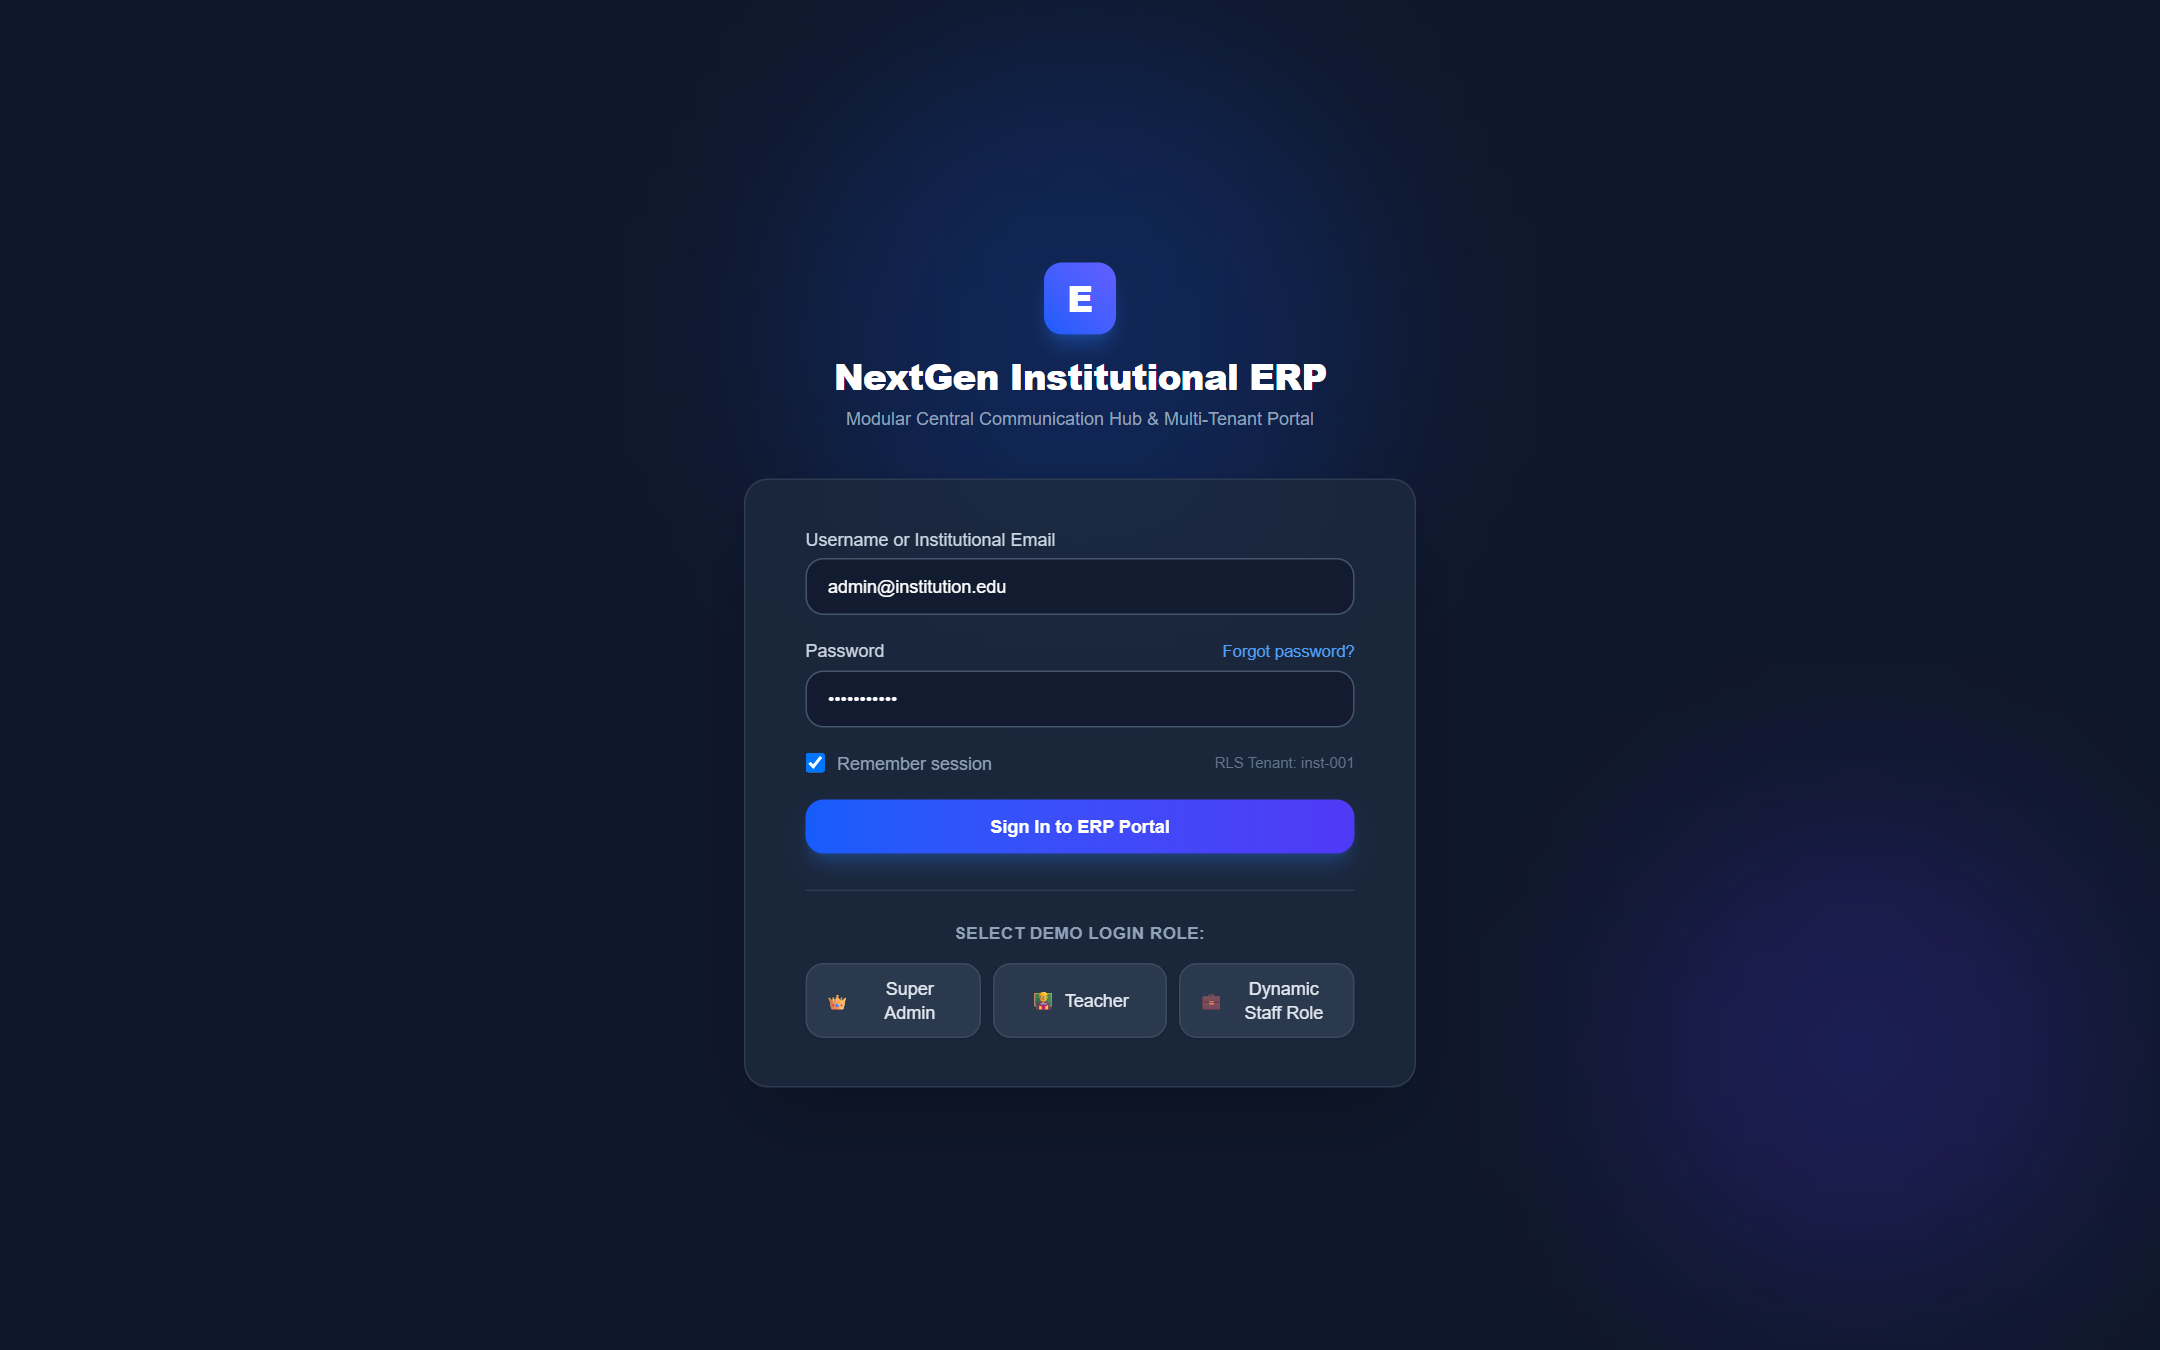
\includegraphics[width=\textwidth]{book_figures/screens/s01_login.png}
    \caption{Sign-in page}
    \label{fig:impl-login}
\end{figure}

After signing in, administrators and staff reach the dashboard in Figure~\ref{fig:impl-dashboard}. It shows the institution's name and summary figures, such as the number of students and teachers and today's attendance, which are read from the Core API, together with shortcuts to the main modules. The navigation shows only the modules that the user's role and the institution's subscription allow.

\begin{figure}[H]
    \centering
    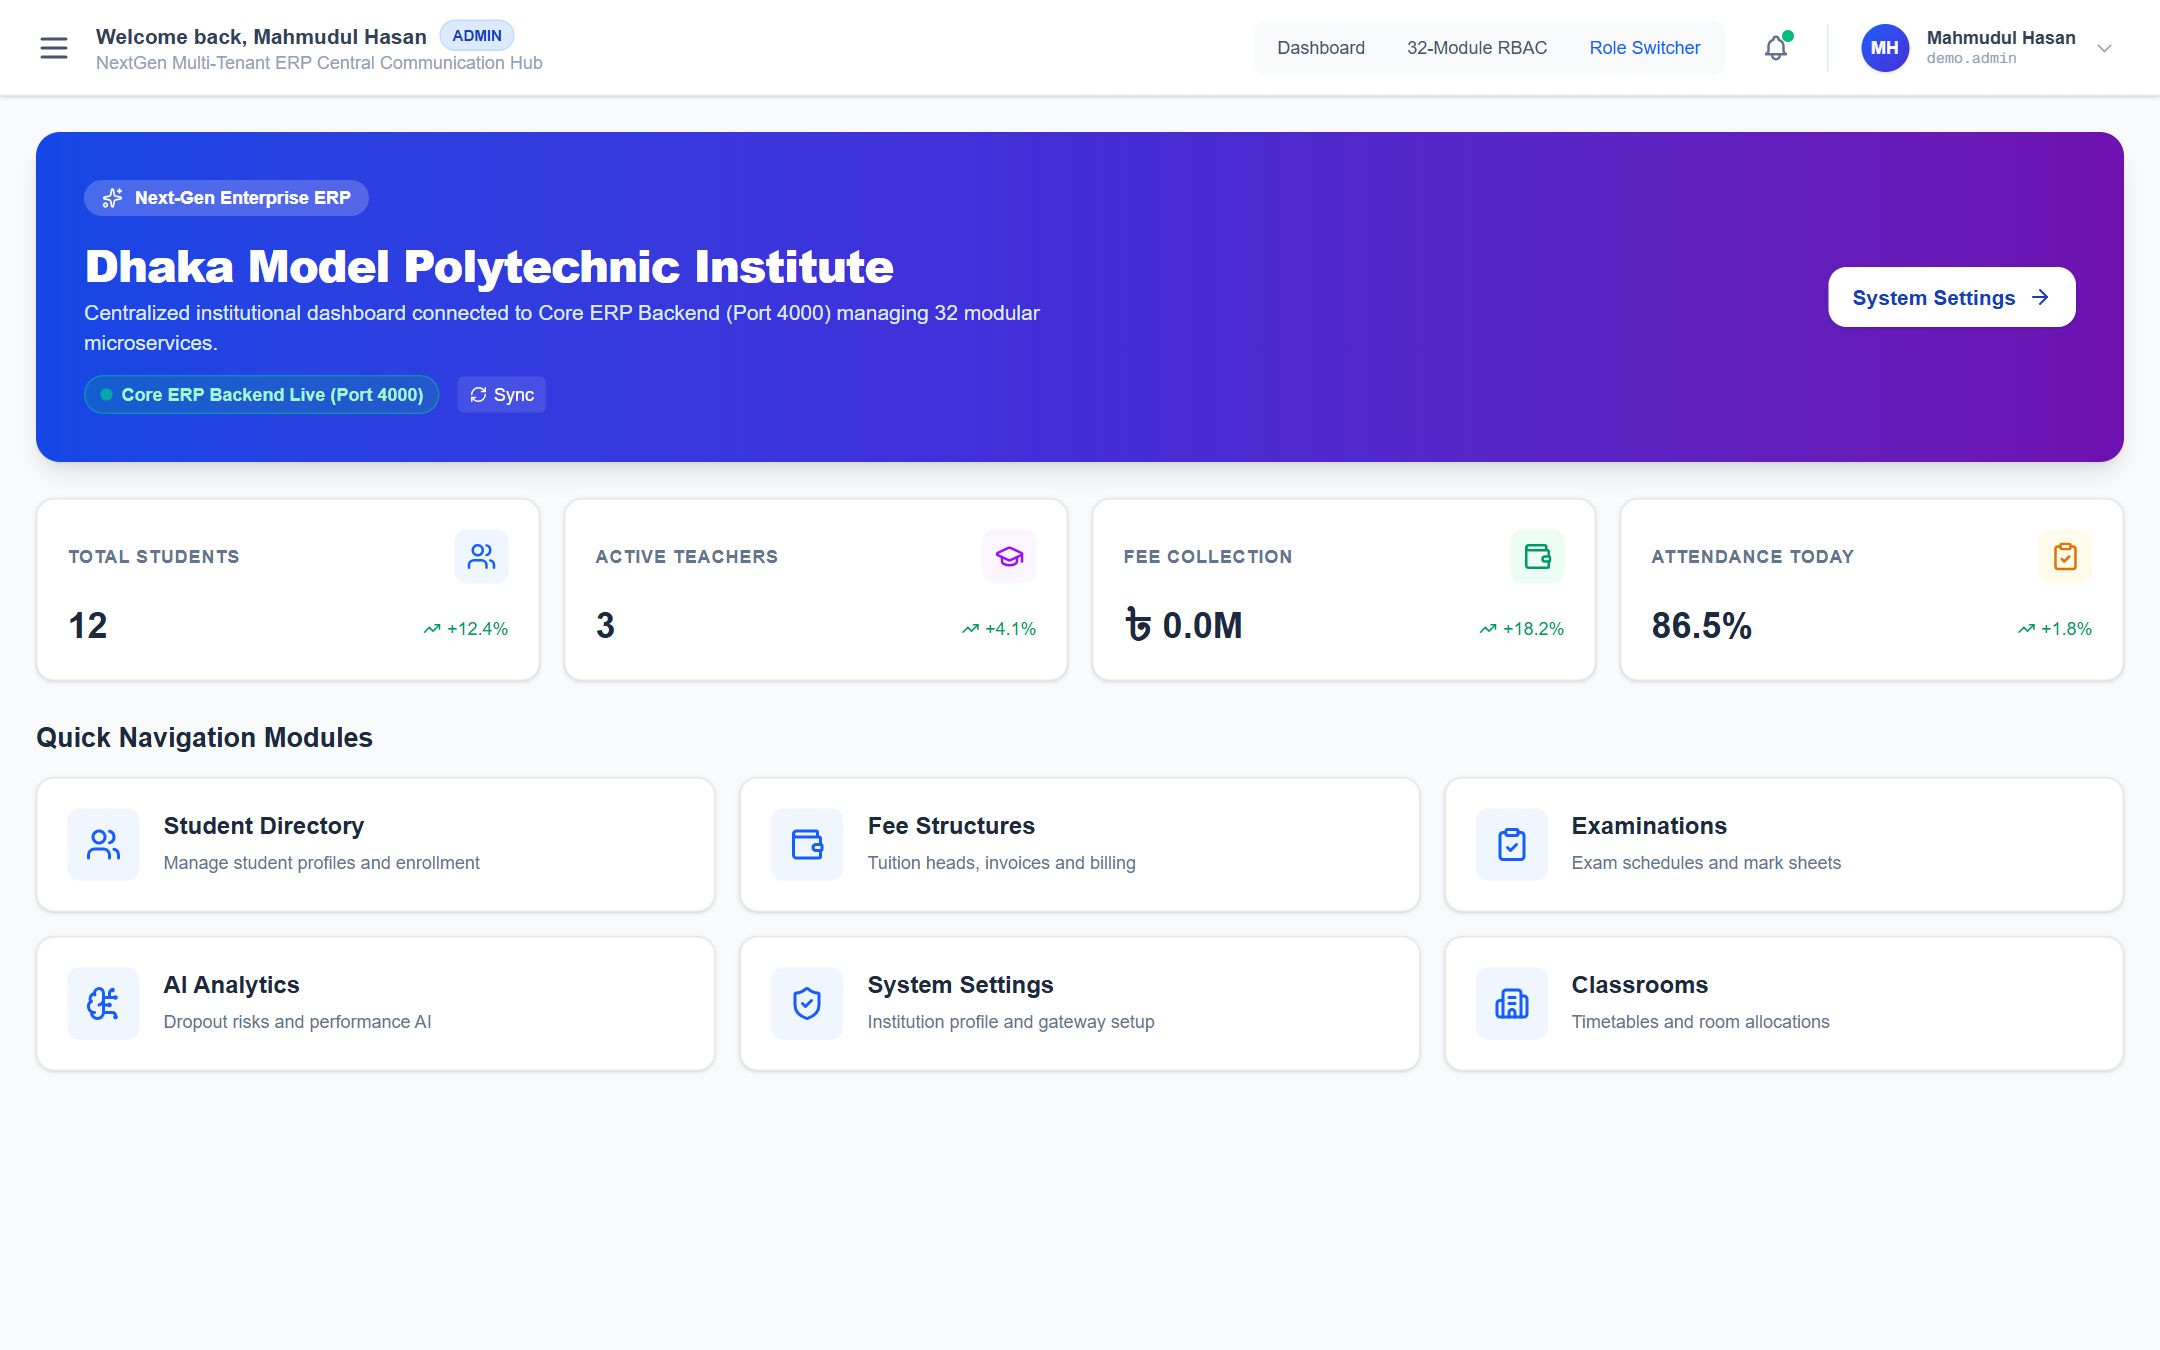
\includegraphics[width=\textwidth]{book_figures/screens/s02_admin_dashboard.png}
    \caption{Administration dashboard}
    \label{fig:impl-dashboard}
\end{figure}

\section{Institution Registration and Platform Management}
A new institution joins the platform from the public registration page in Figure~\ref{fig:impl-register}. The person registering enters the institution's name, short code, type and contact details, chooses the modules the institution needs and a monthly or yearly billing cycle, and sees the price of each module. The price quote is calculated by the Core API from the module prices, and a yearly subscription is charged for ten months. After submission, the institution stays pending until the Super Admin approves it, and only then can its administrator sign in.

\begin{figure}[H]
    \centering
    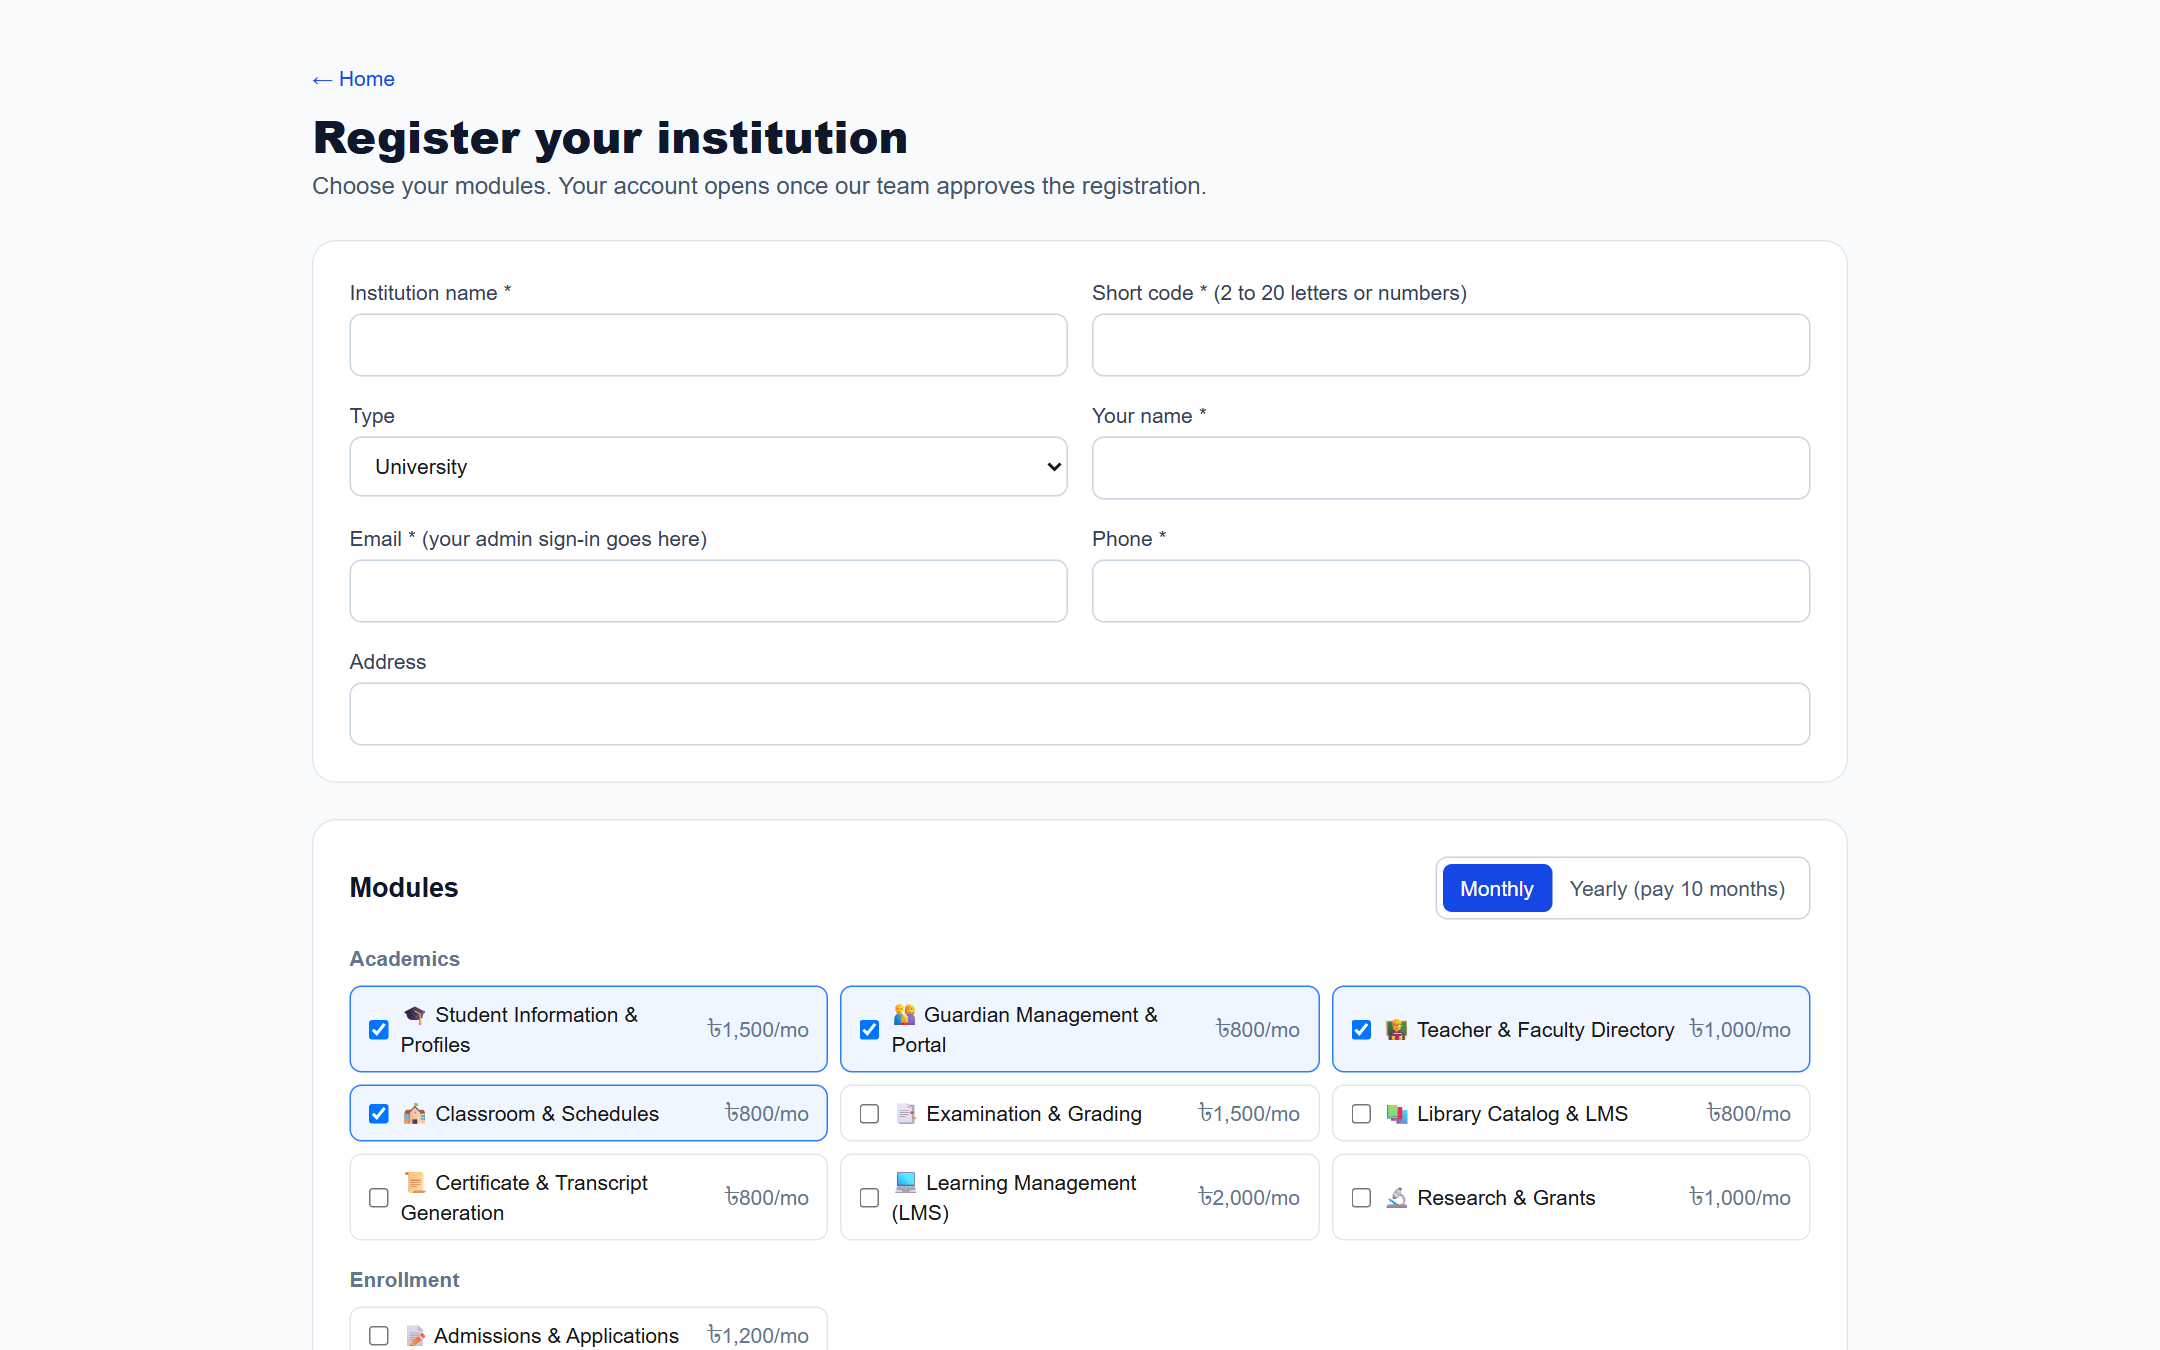
\includegraphics[width=\textwidth]{book_figures/screens/s27_register.png}
    \caption{Institution registration with module selection}
    \label{fig:impl-register}
\end{figure}

The Super Admin manages the platform from the Platform page, which has tabs for registration and subscription requests, institutions, subscription billing and module prices. Figure~\ref{fig:impl-pricing} shows the Module Prices tab, where the monthly price of each module is set and a module can be offered or withdrawn. Core modules, such as system configuration and institution setup, are included at no charge. The registration page reads these prices from the server, so a price change applies to every new quote at once.

\begin{figure}[H]
    \centering
    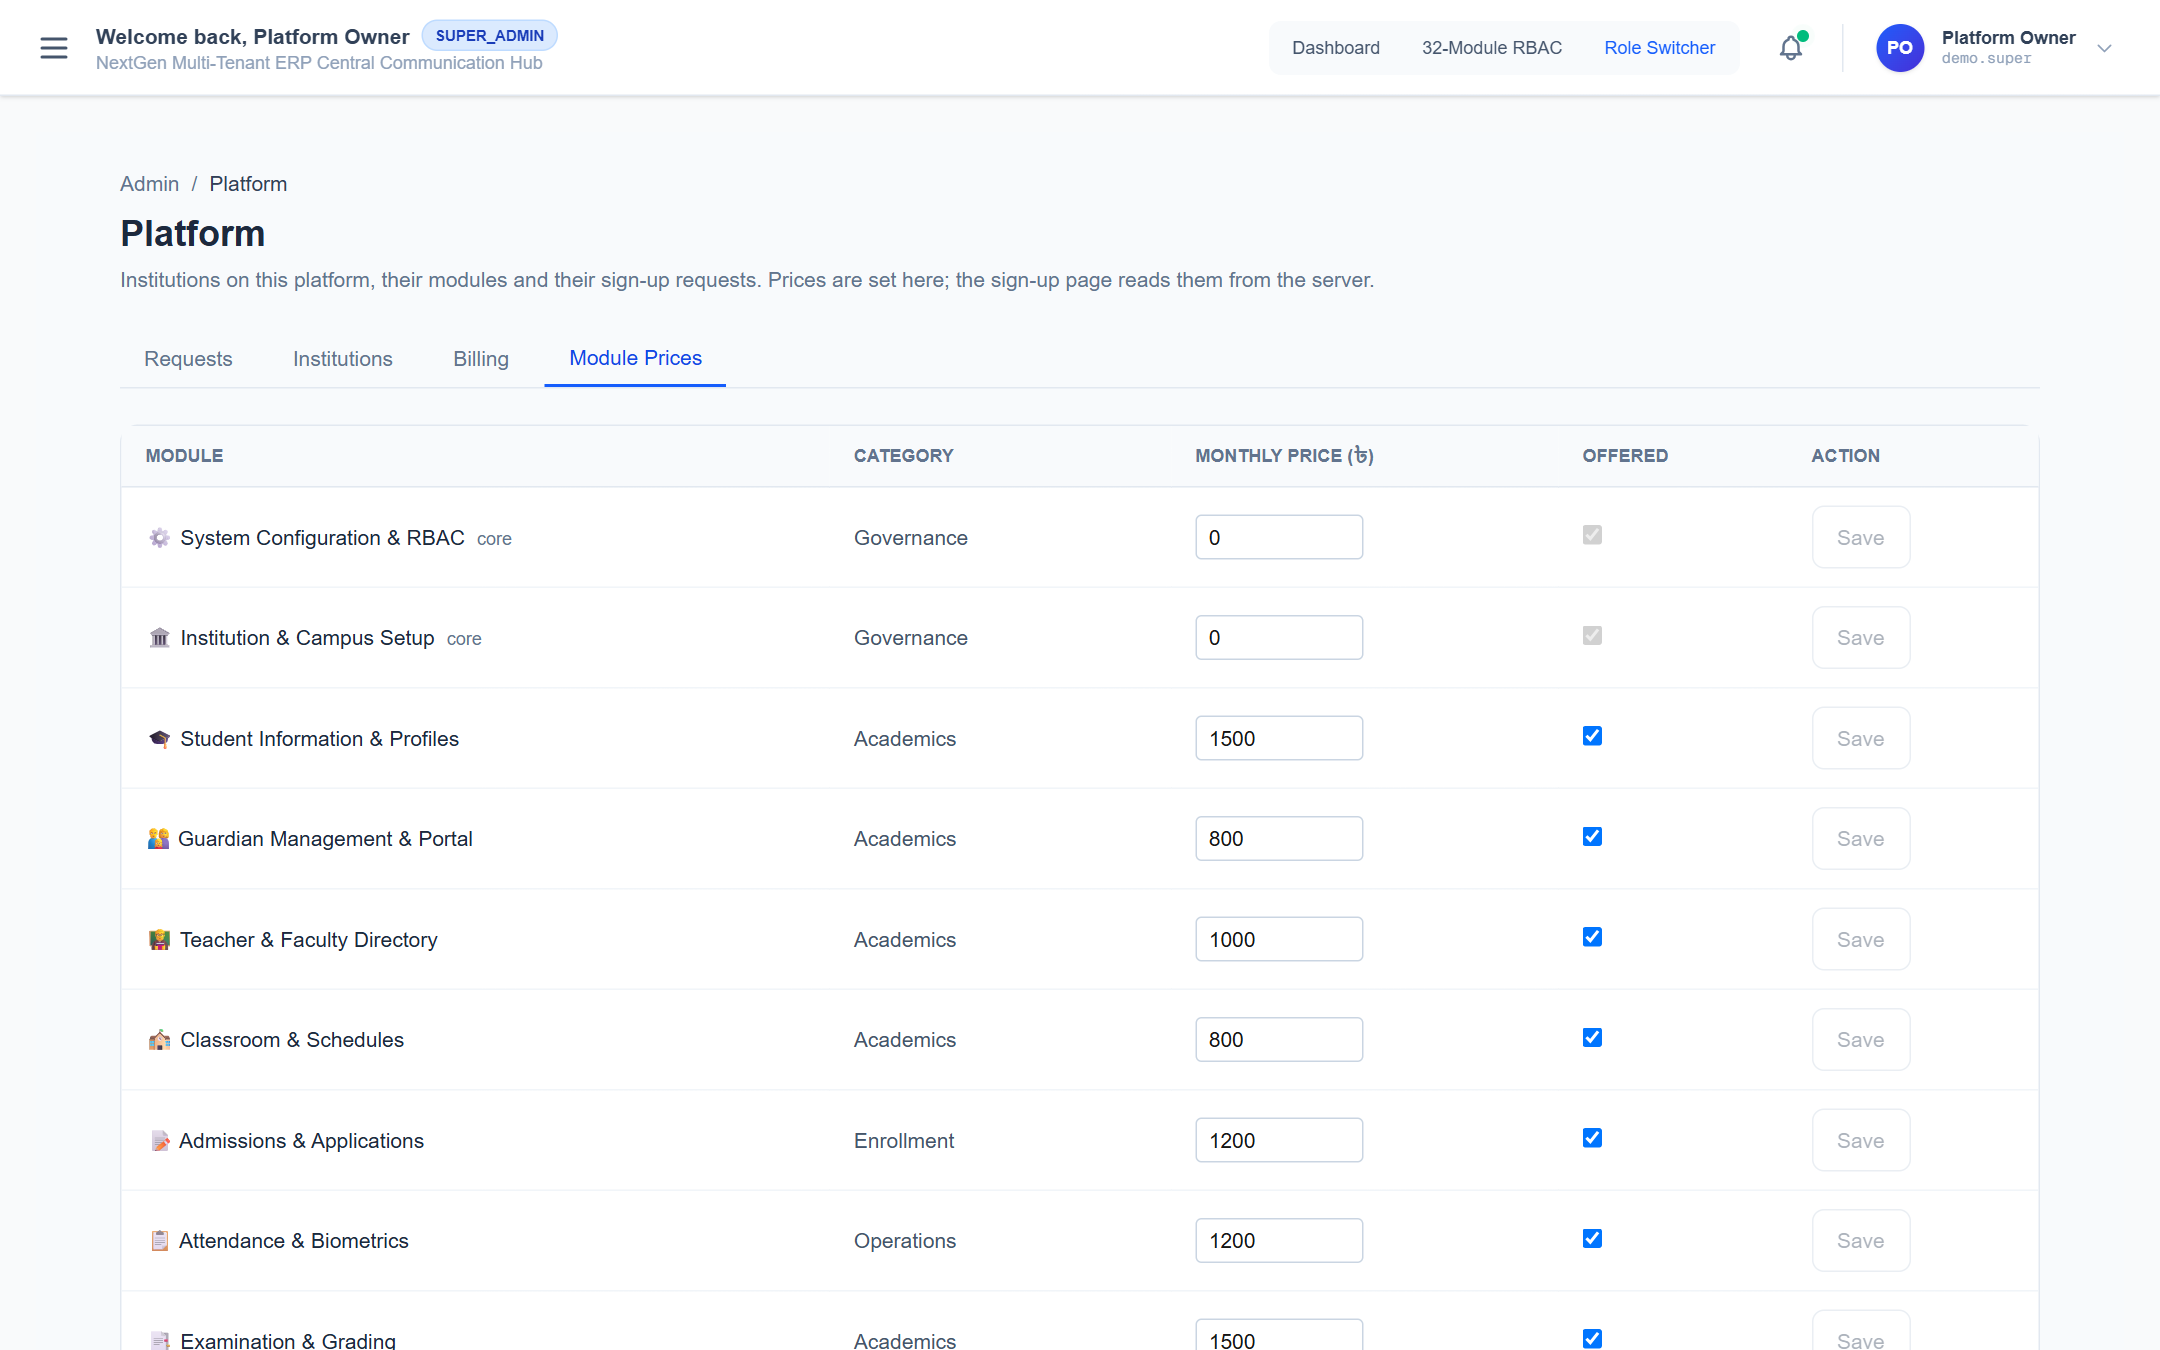
\includegraphics[width=\textwidth]{book_figures/screens/s26_platform_pricing.png}
    \caption{Module prices on the Platform page}
    \label{fig:impl-pricing}
\end{figure}

\section{User, Role and Permission Management}
The Users and Accounts screen in Figure~\ref{fig:impl-users} lists every account of the institution with its role, status and last sign-in, and allows administrators to create accounts, reset passwords, view activity and manage a user's permissions. When an account is created, the Core API generates a temporary password and sends it only to the person's email address; the screen shows whether the sign-in details were delivered.

\begin{figure}[H]
    \centering
    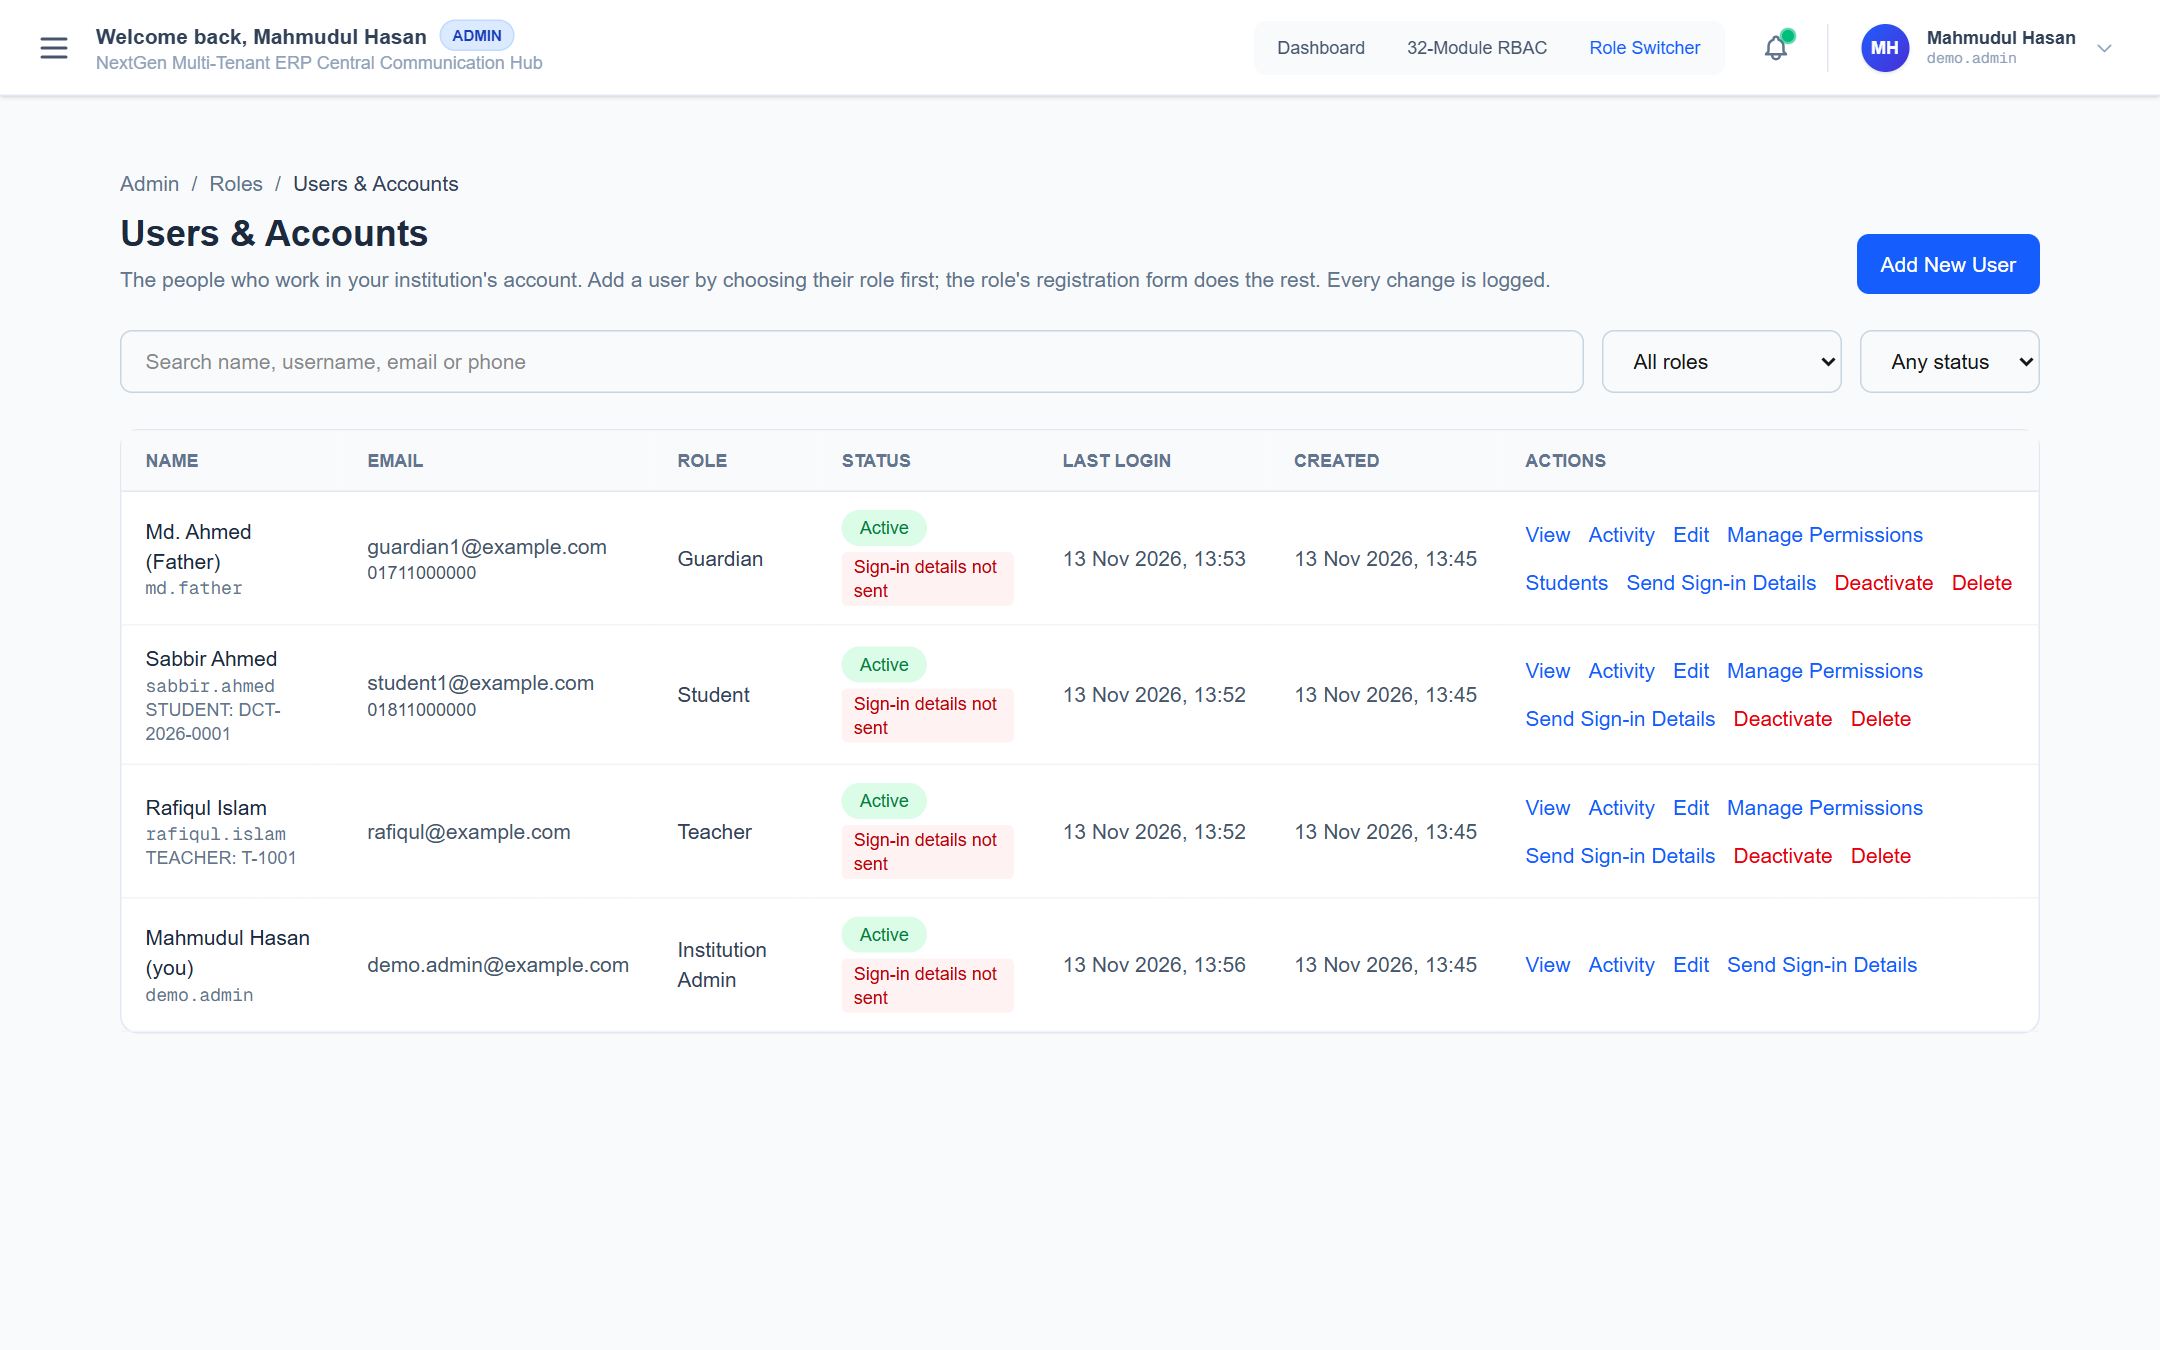
\includegraphics[width=\textwidth]{book_figures/screens/s03_users.png}
    \caption{Users and accounts}
    \label{fig:impl-users}
\end{figure}

The Roles and Permissions screen in Figure~\ref{fig:impl-roles} lists the built-in roles and any custom roles of the institution. Selecting a role shows its permissions as a tree of modules and actions. Built-in roles are read-only, while custom roles can be created, cloned and edited. The same permission keys are checked by the Core API on every request, so the screen and the server always apply the same rules.

\begin{figure}[H]
    \centering
    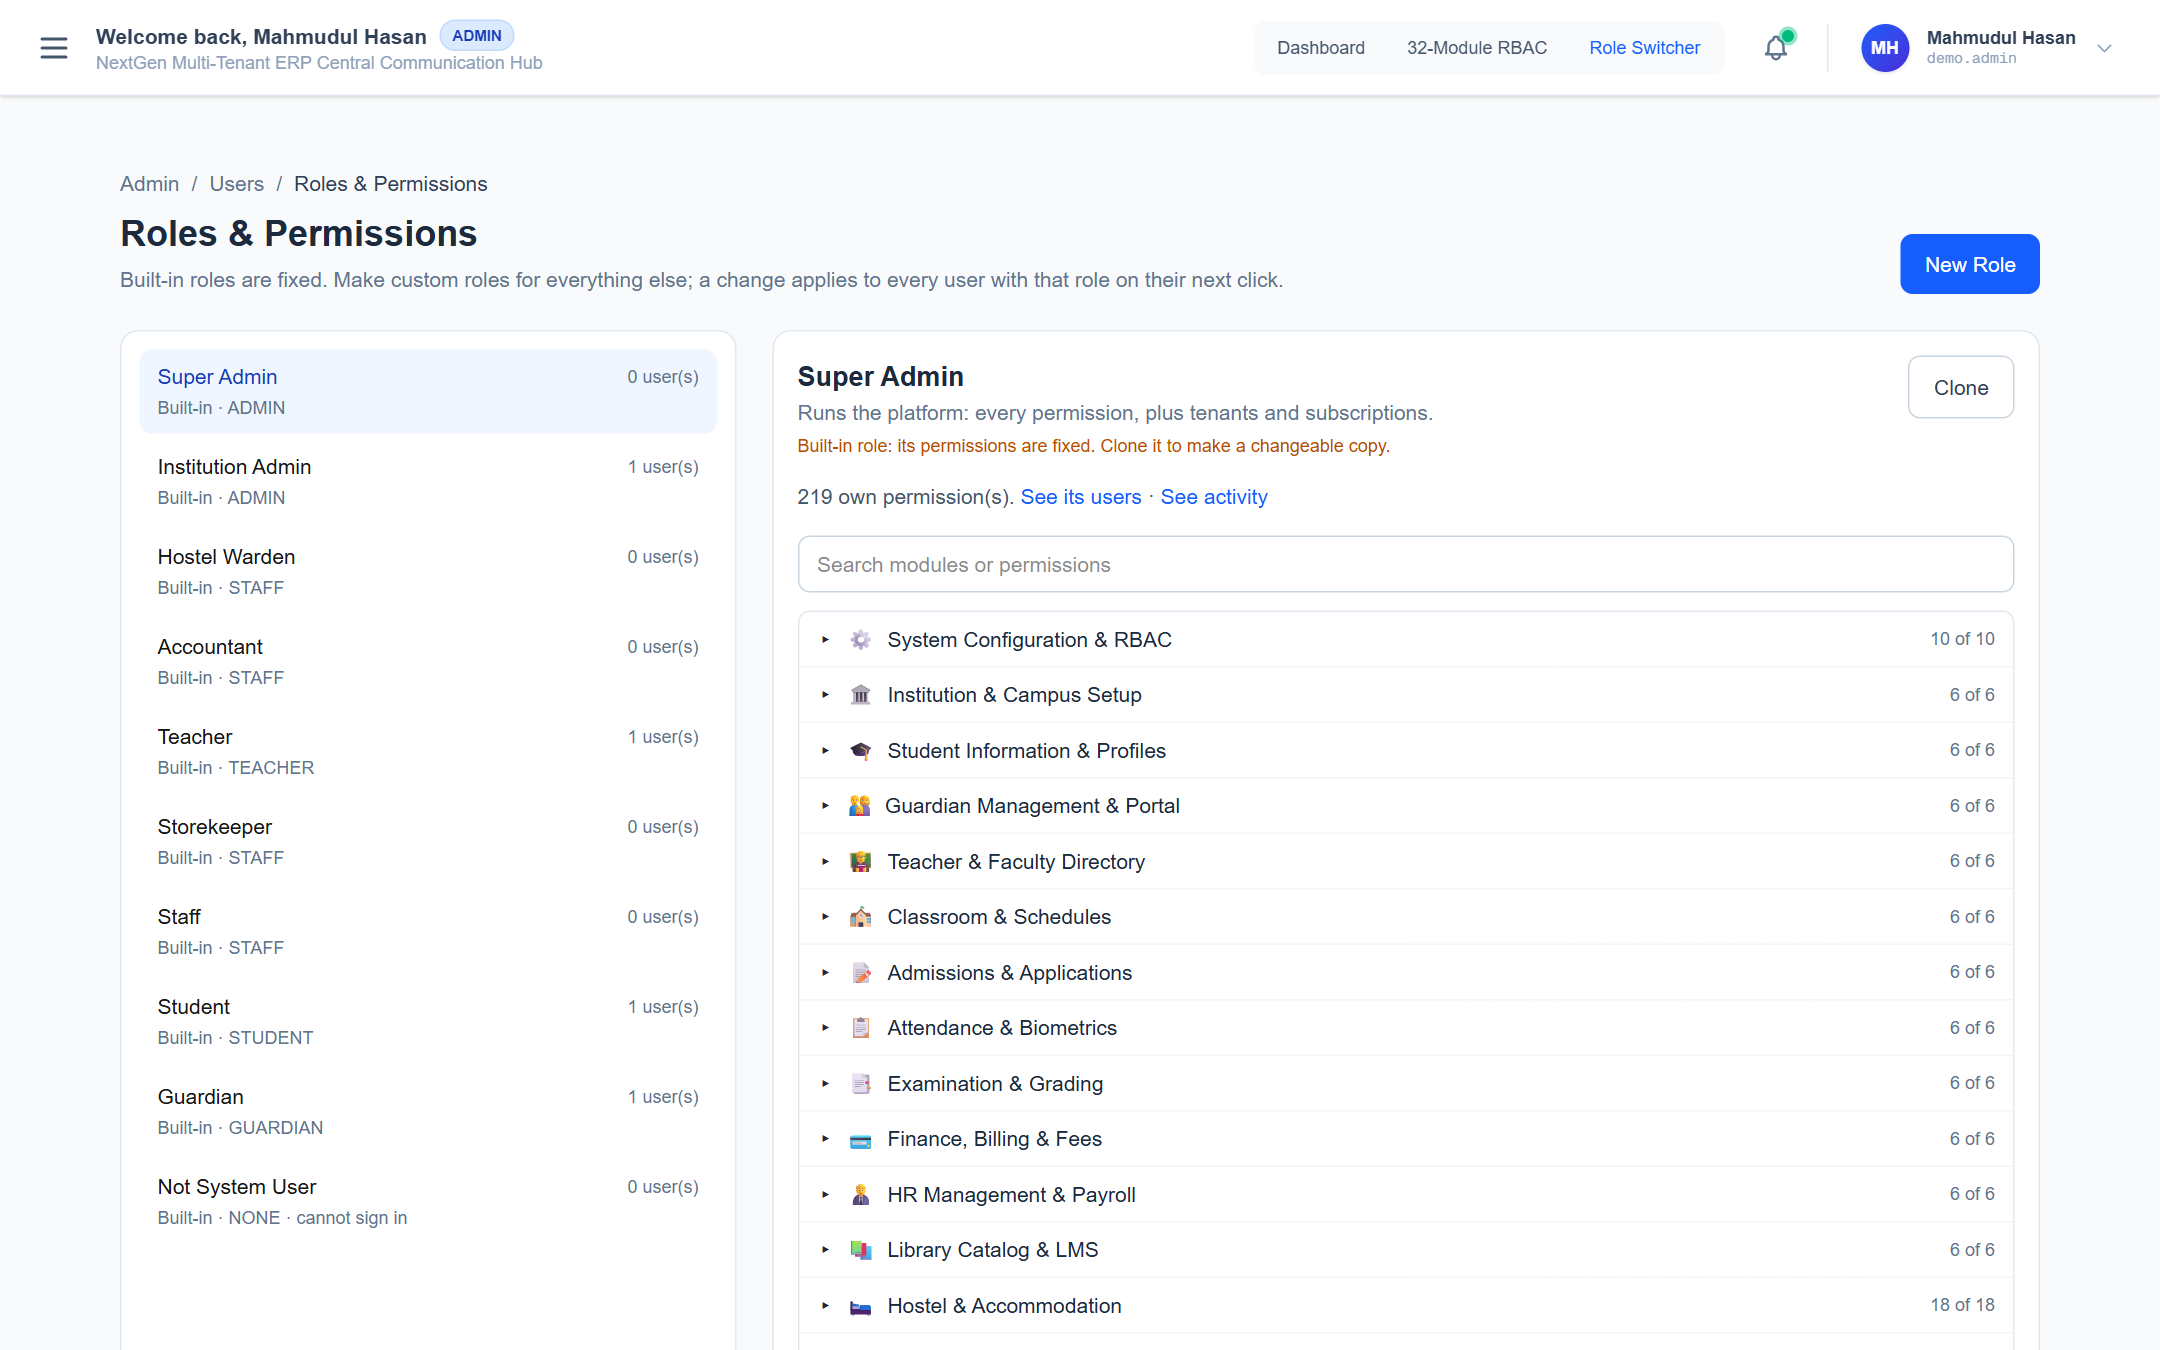
\includegraphics[width=\textwidth]{book_figures/screens/s04_roles.png}
    \caption{Roles and permissions}
    \label{fig:impl-roles}
\end{figure}

\section{Dynamic Form Builder}
The Form Builder in Figure~\ref{fig:impl-forms} lists the institution's own forms with their status and version. In the demonstration, a transport pass application form has been published and a lab equipment request form is still a draft. Administrators add fields of ten types, including select, radio, checkbox and multi-select fields with options, and can show a field only when an earlier answer has a given value. Publishing a form fixes its current version; later edits create a new draft version, and every submission is checked by the Core API against the version it was made with.

\begin{figure}[H]
    \centering
    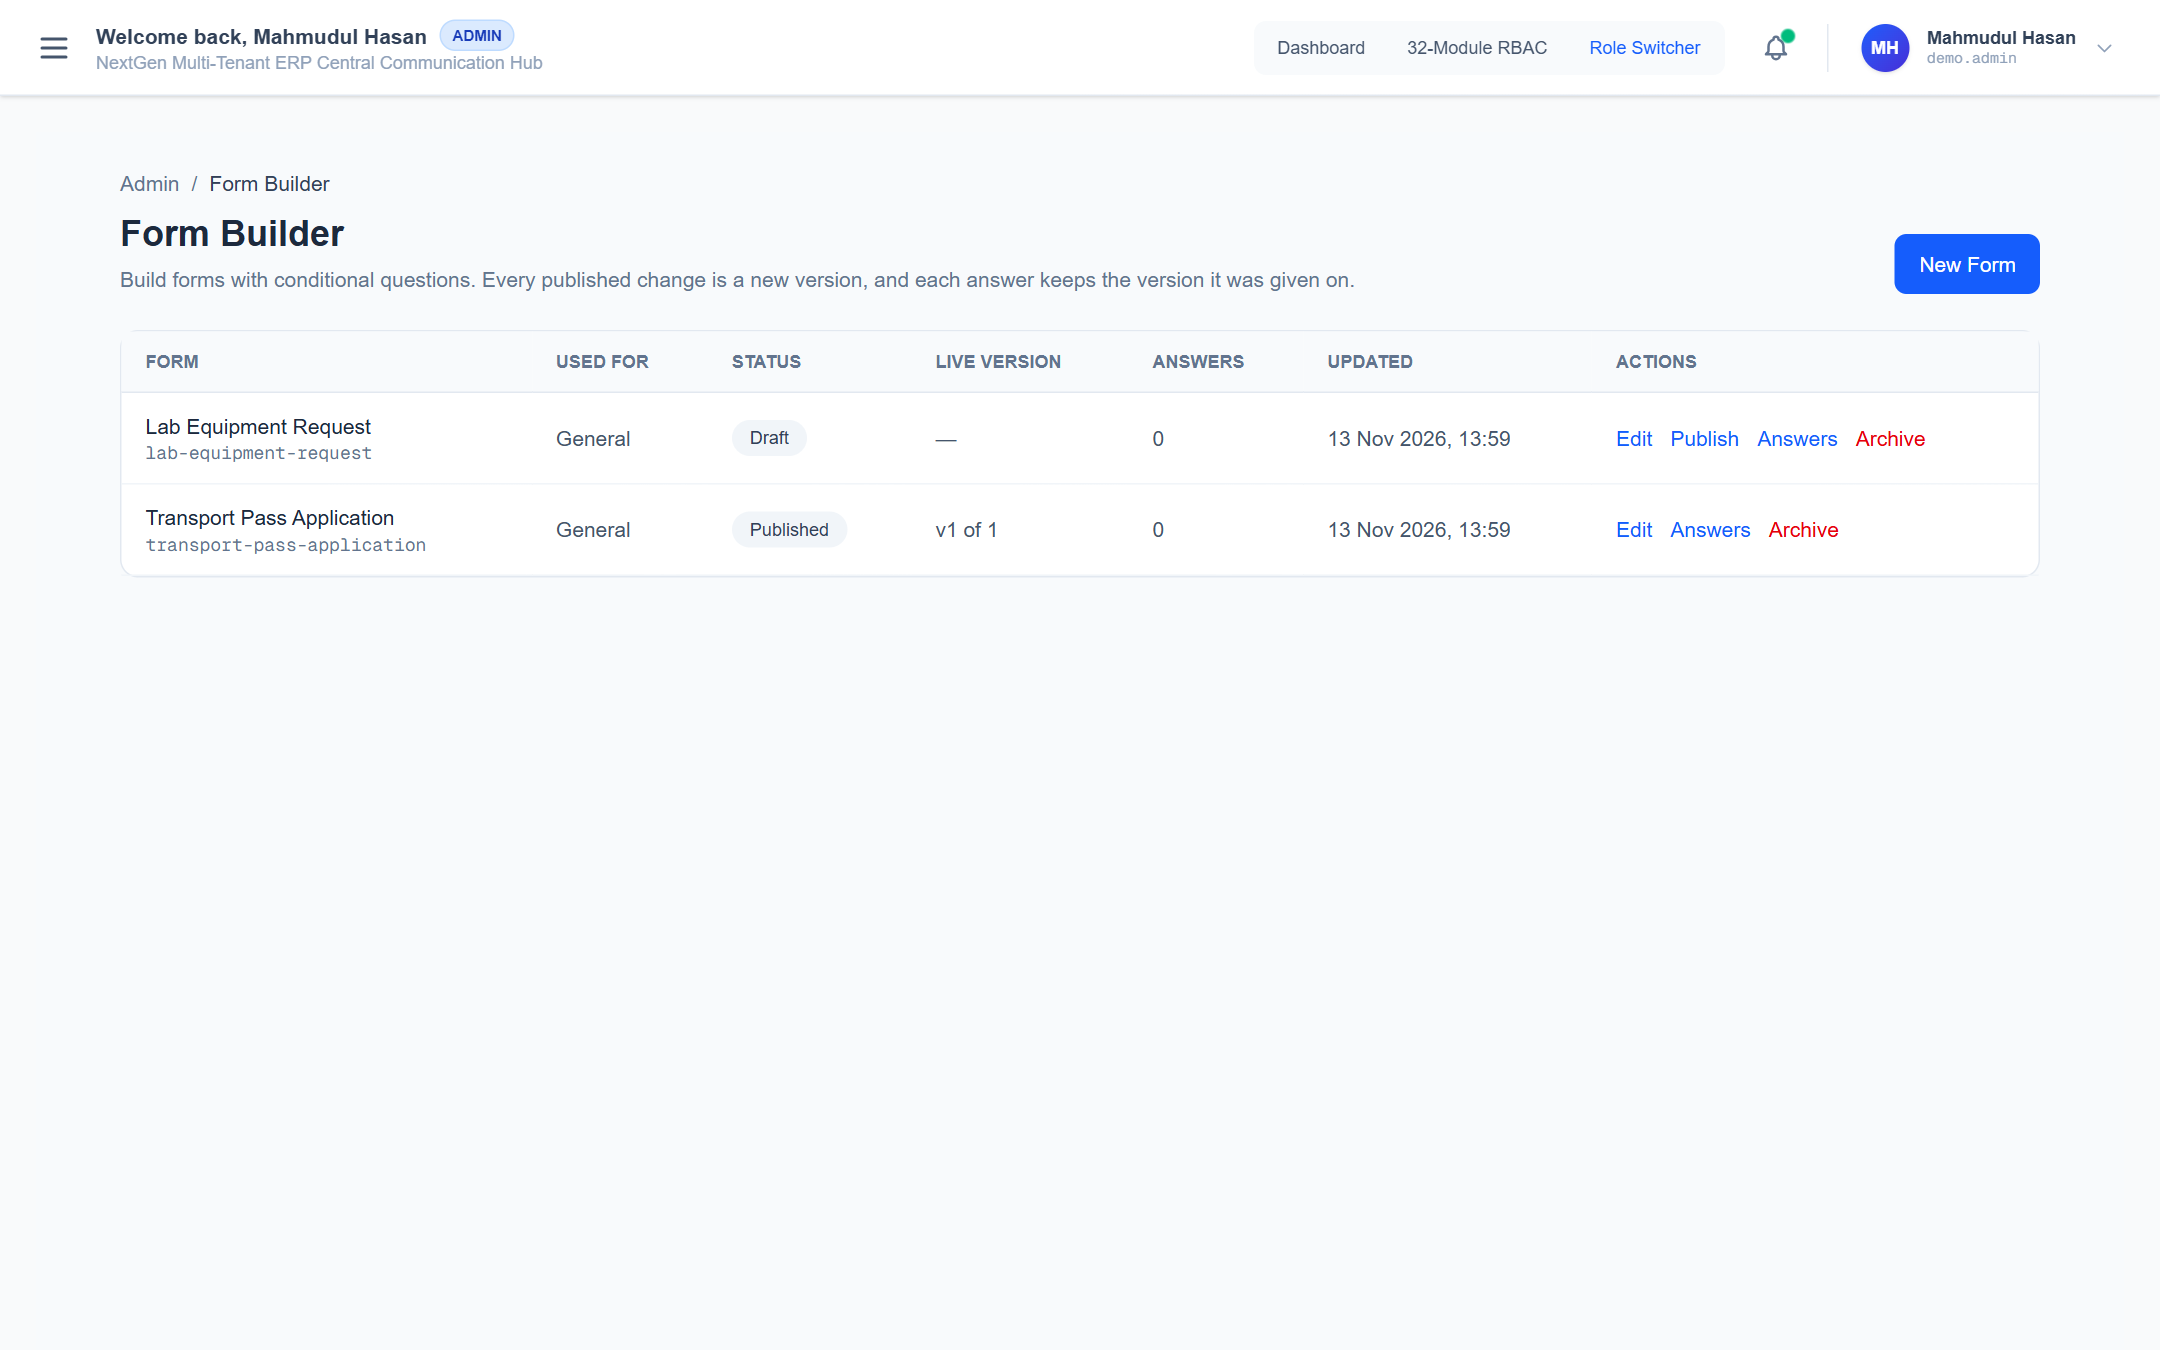
\includegraphics[width=\textwidth]{book_figures/screens/s05_form_builder.png}
    \caption{Dynamic form builder}
    \label{fig:impl-forms}
\end{figure}

\section{Academic Structure and Student Management}
The Academic Structure screen in Figure~\ref{fig:impl-academic} manages departments, programs, sessions, sections, courses and classes through tabs that share one generic implementation in the Core API. The demonstration institution has the Computer Technology and Electrical Technology departments, each with a diploma program.

\begin{figure}[H]
    \centering
    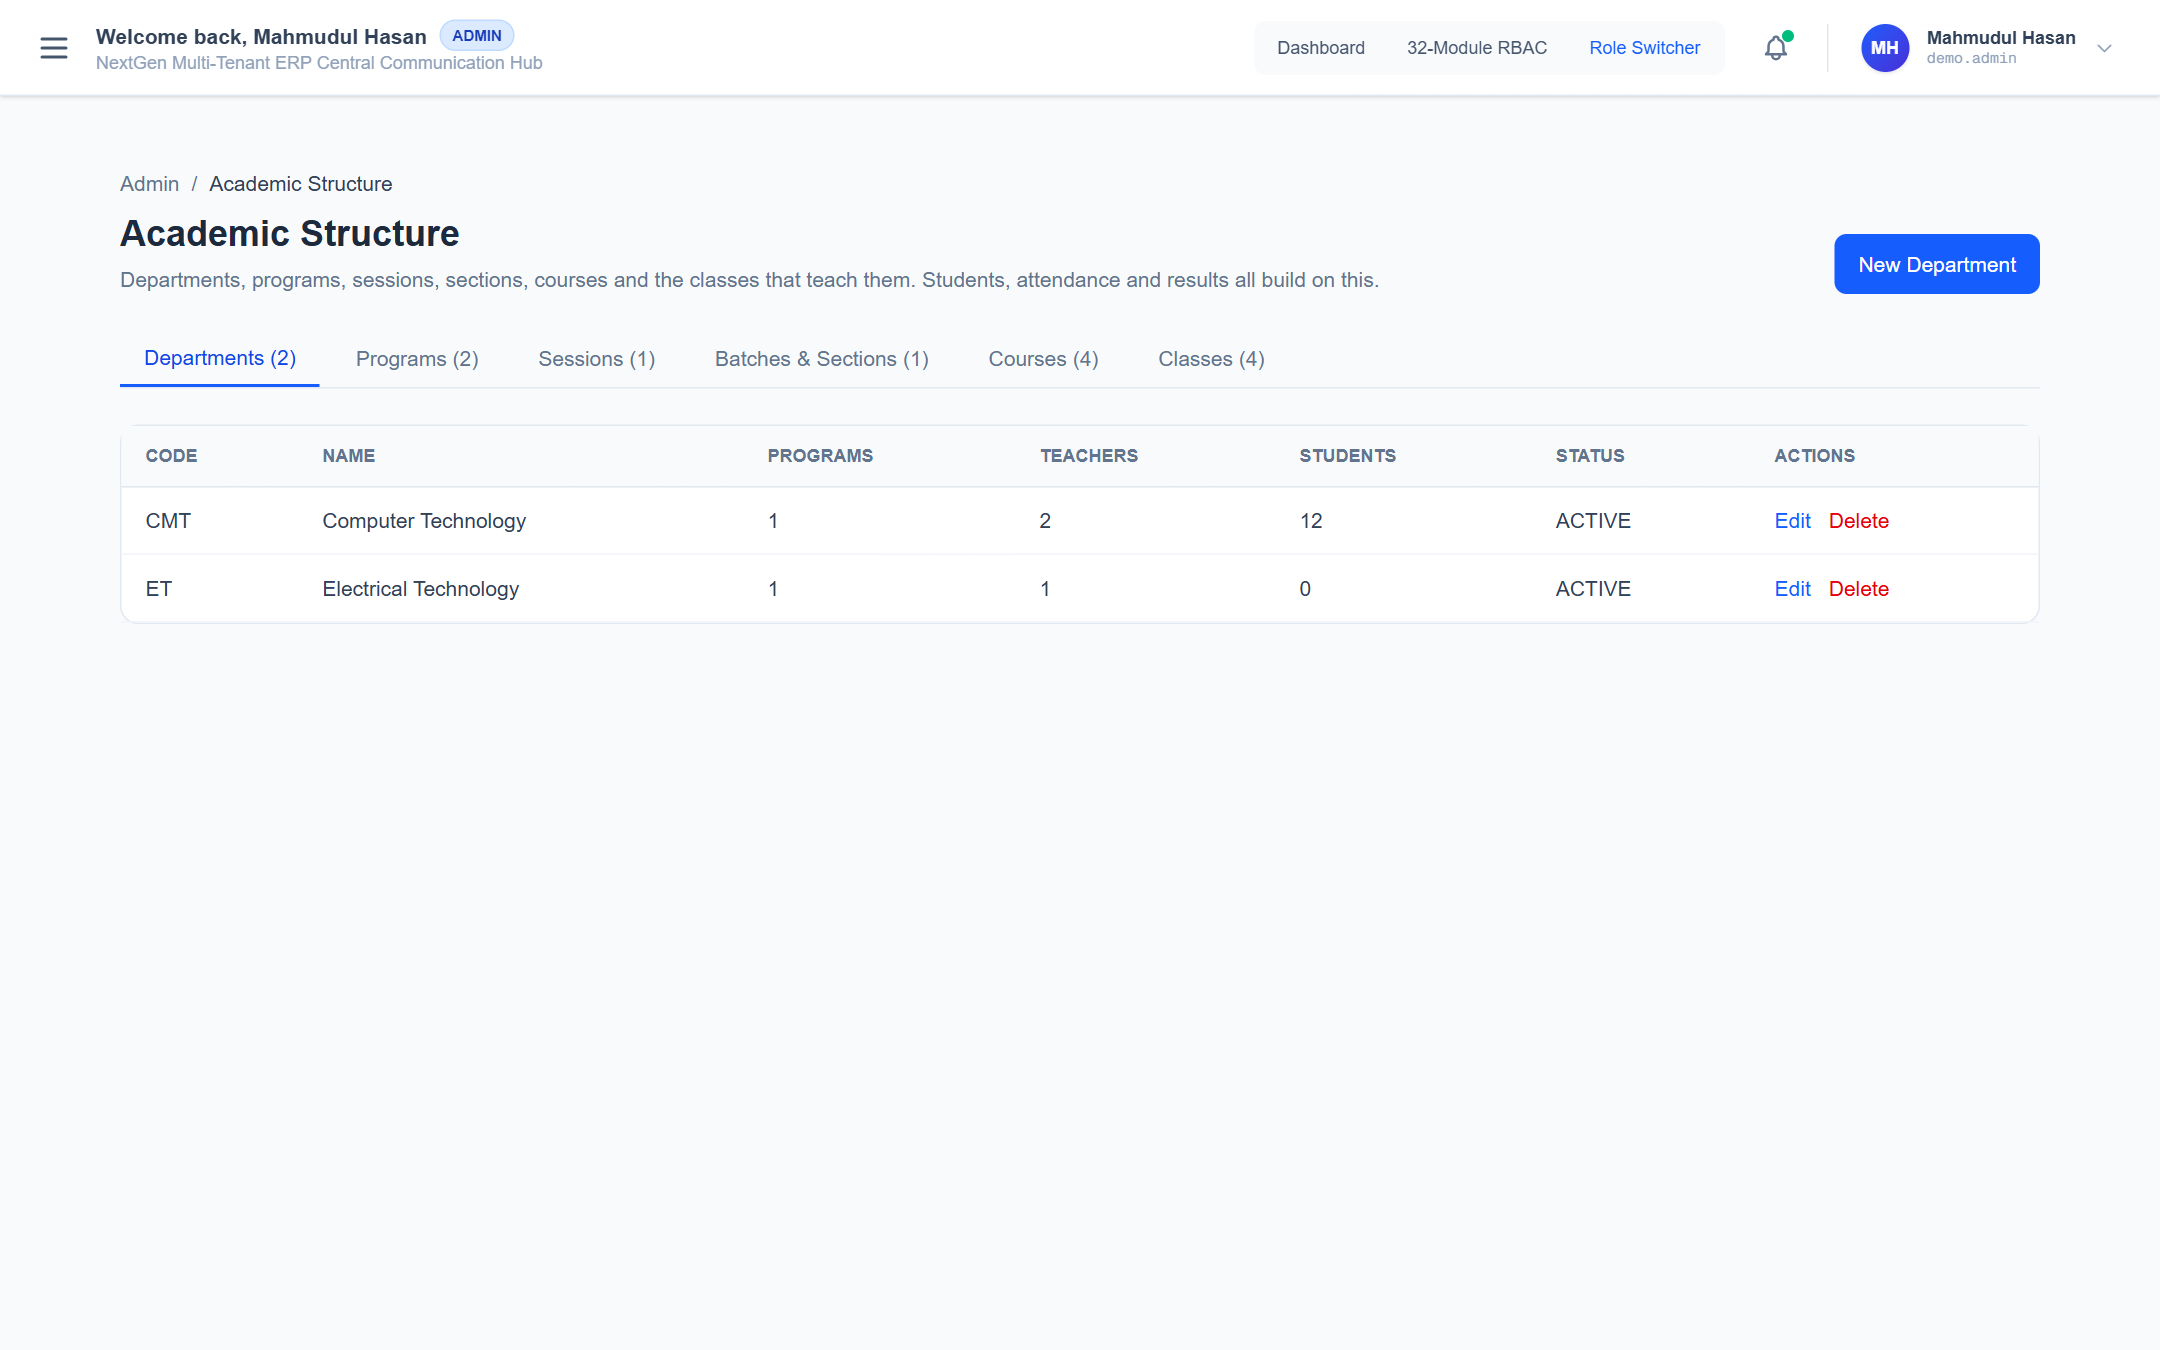
\includegraphics[width=\textwidth]{book_figures/screens/s06_academic_structure.png}
    \caption{Academic structure}
    \label{fig:impl-academic}
\end{figure}

The Students screen in Figure~\ref{fig:impl-students} lists students with their student numbers, which the system generates from the program code and year, together with program, section, status and account information. From here, administrators admit students, edit their details and guardian information, change status with a reason, move several students to another section at once, and create portal accounts for a student and the student's guardian.

\begin{figure}[H]
    \centering
    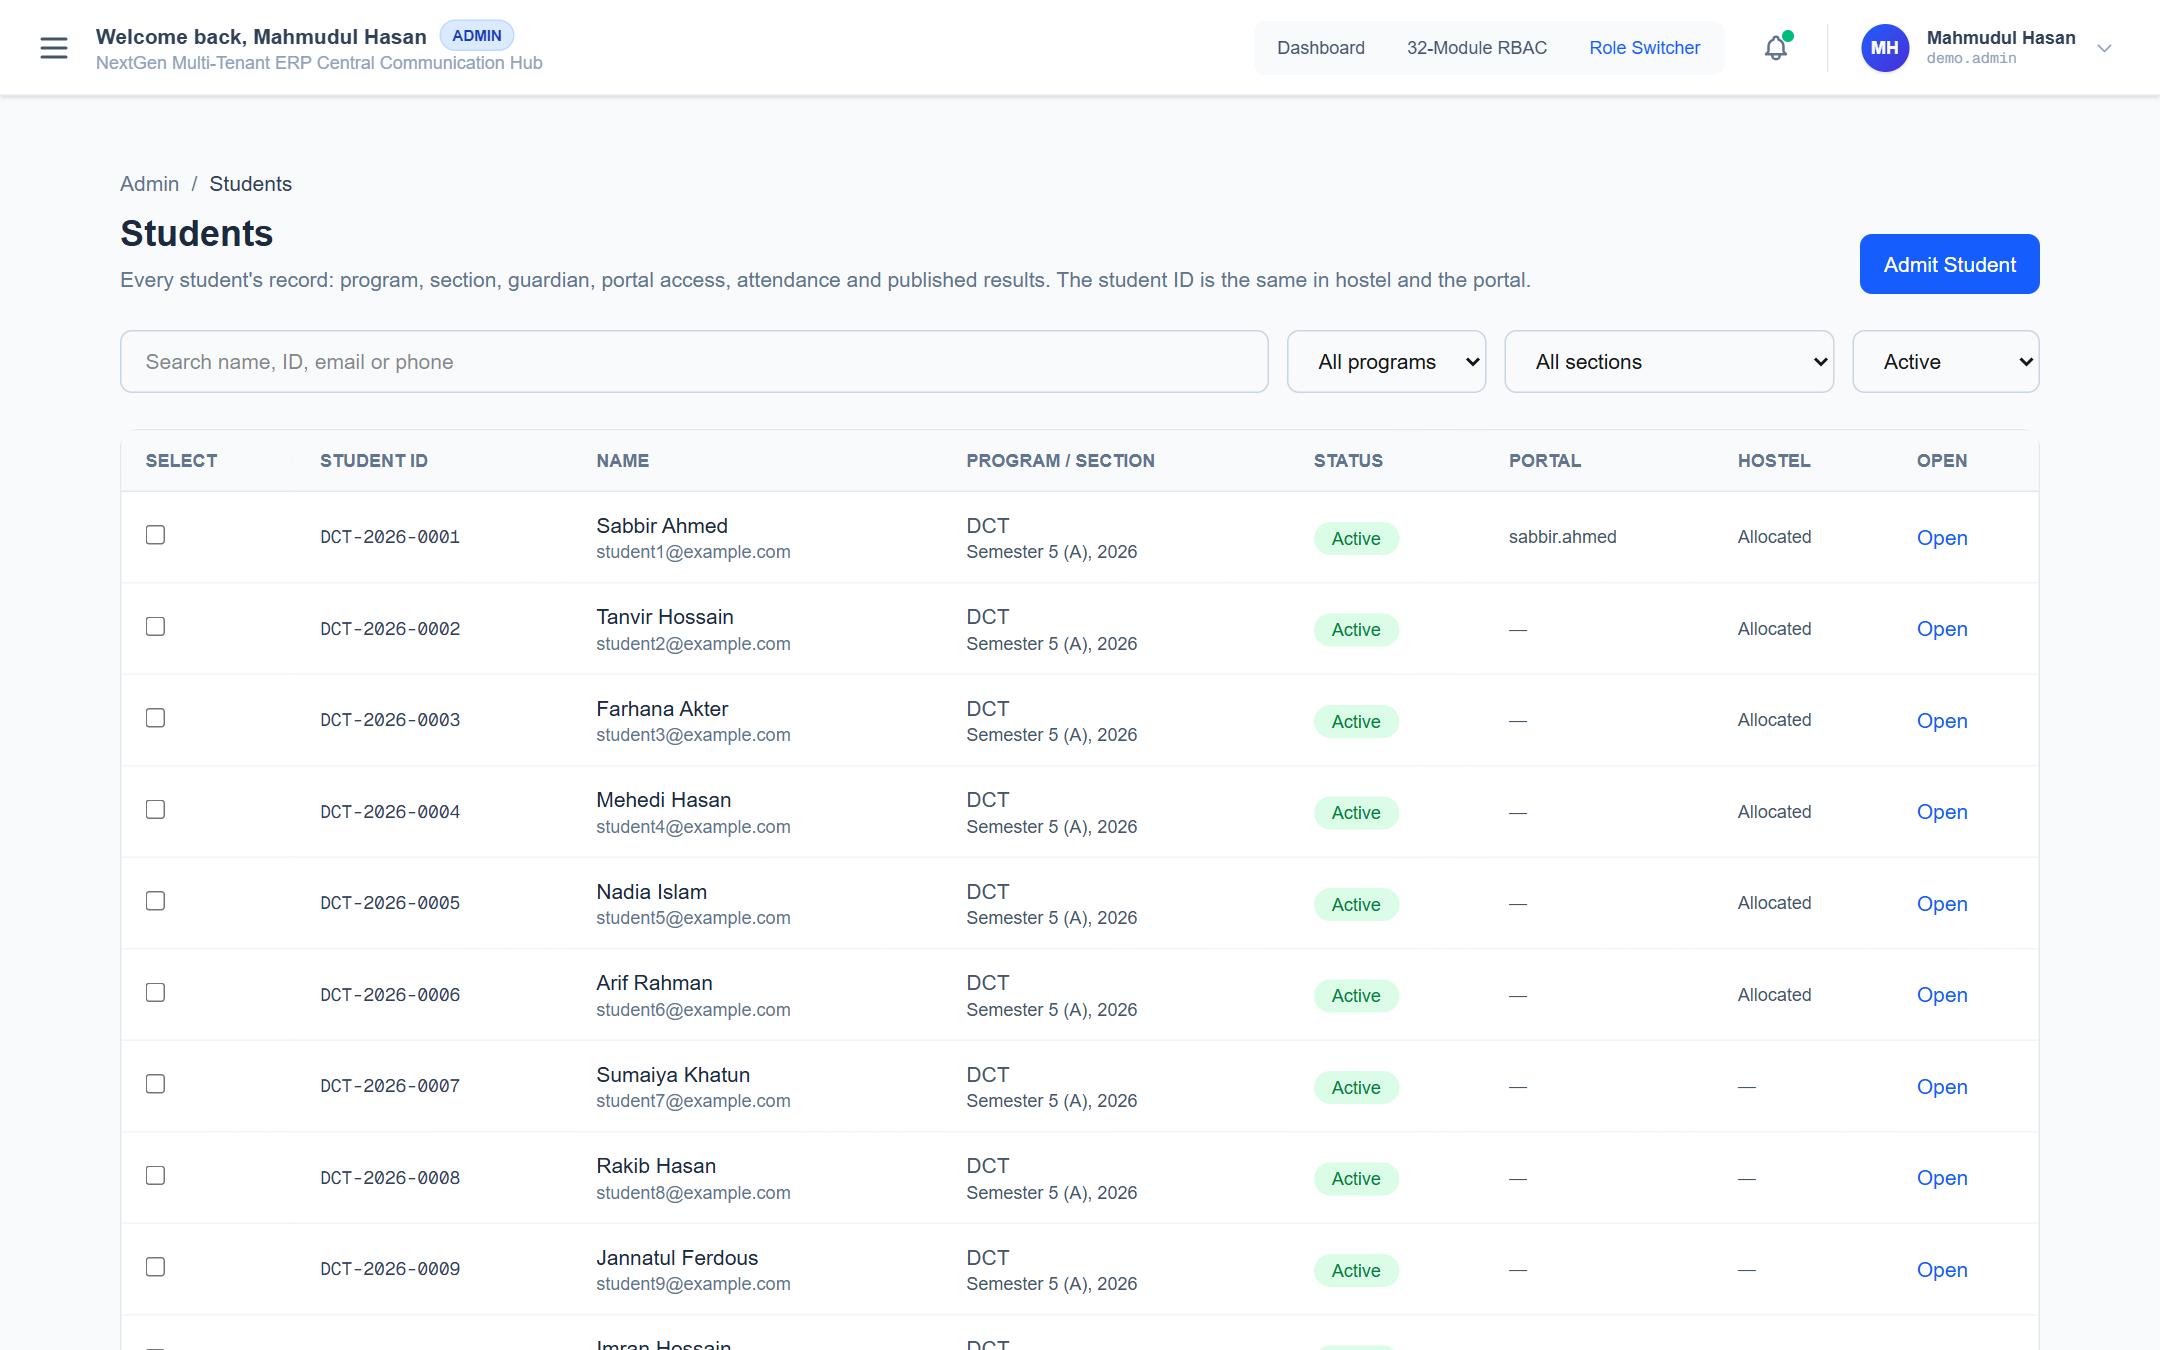
\includegraphics[width=\textwidth]{book_figures/screens/s07_students.png}
    \caption{Student management}
    \label{fig:impl-students}
\end{figure}

\section{Attendance and Examination}
Teachers see only their own classes. On the attendance screen in Figure~\ref{fig:impl-attendance}, signed in as a teacher, the teacher chooses a class and a date, marks each student as present, absent or late, and saves the sheet. The Core API refuses dates in the future and stops a teacher from changing old records, which only administrators can edit.

\begin{figure}[H]
    \centering
    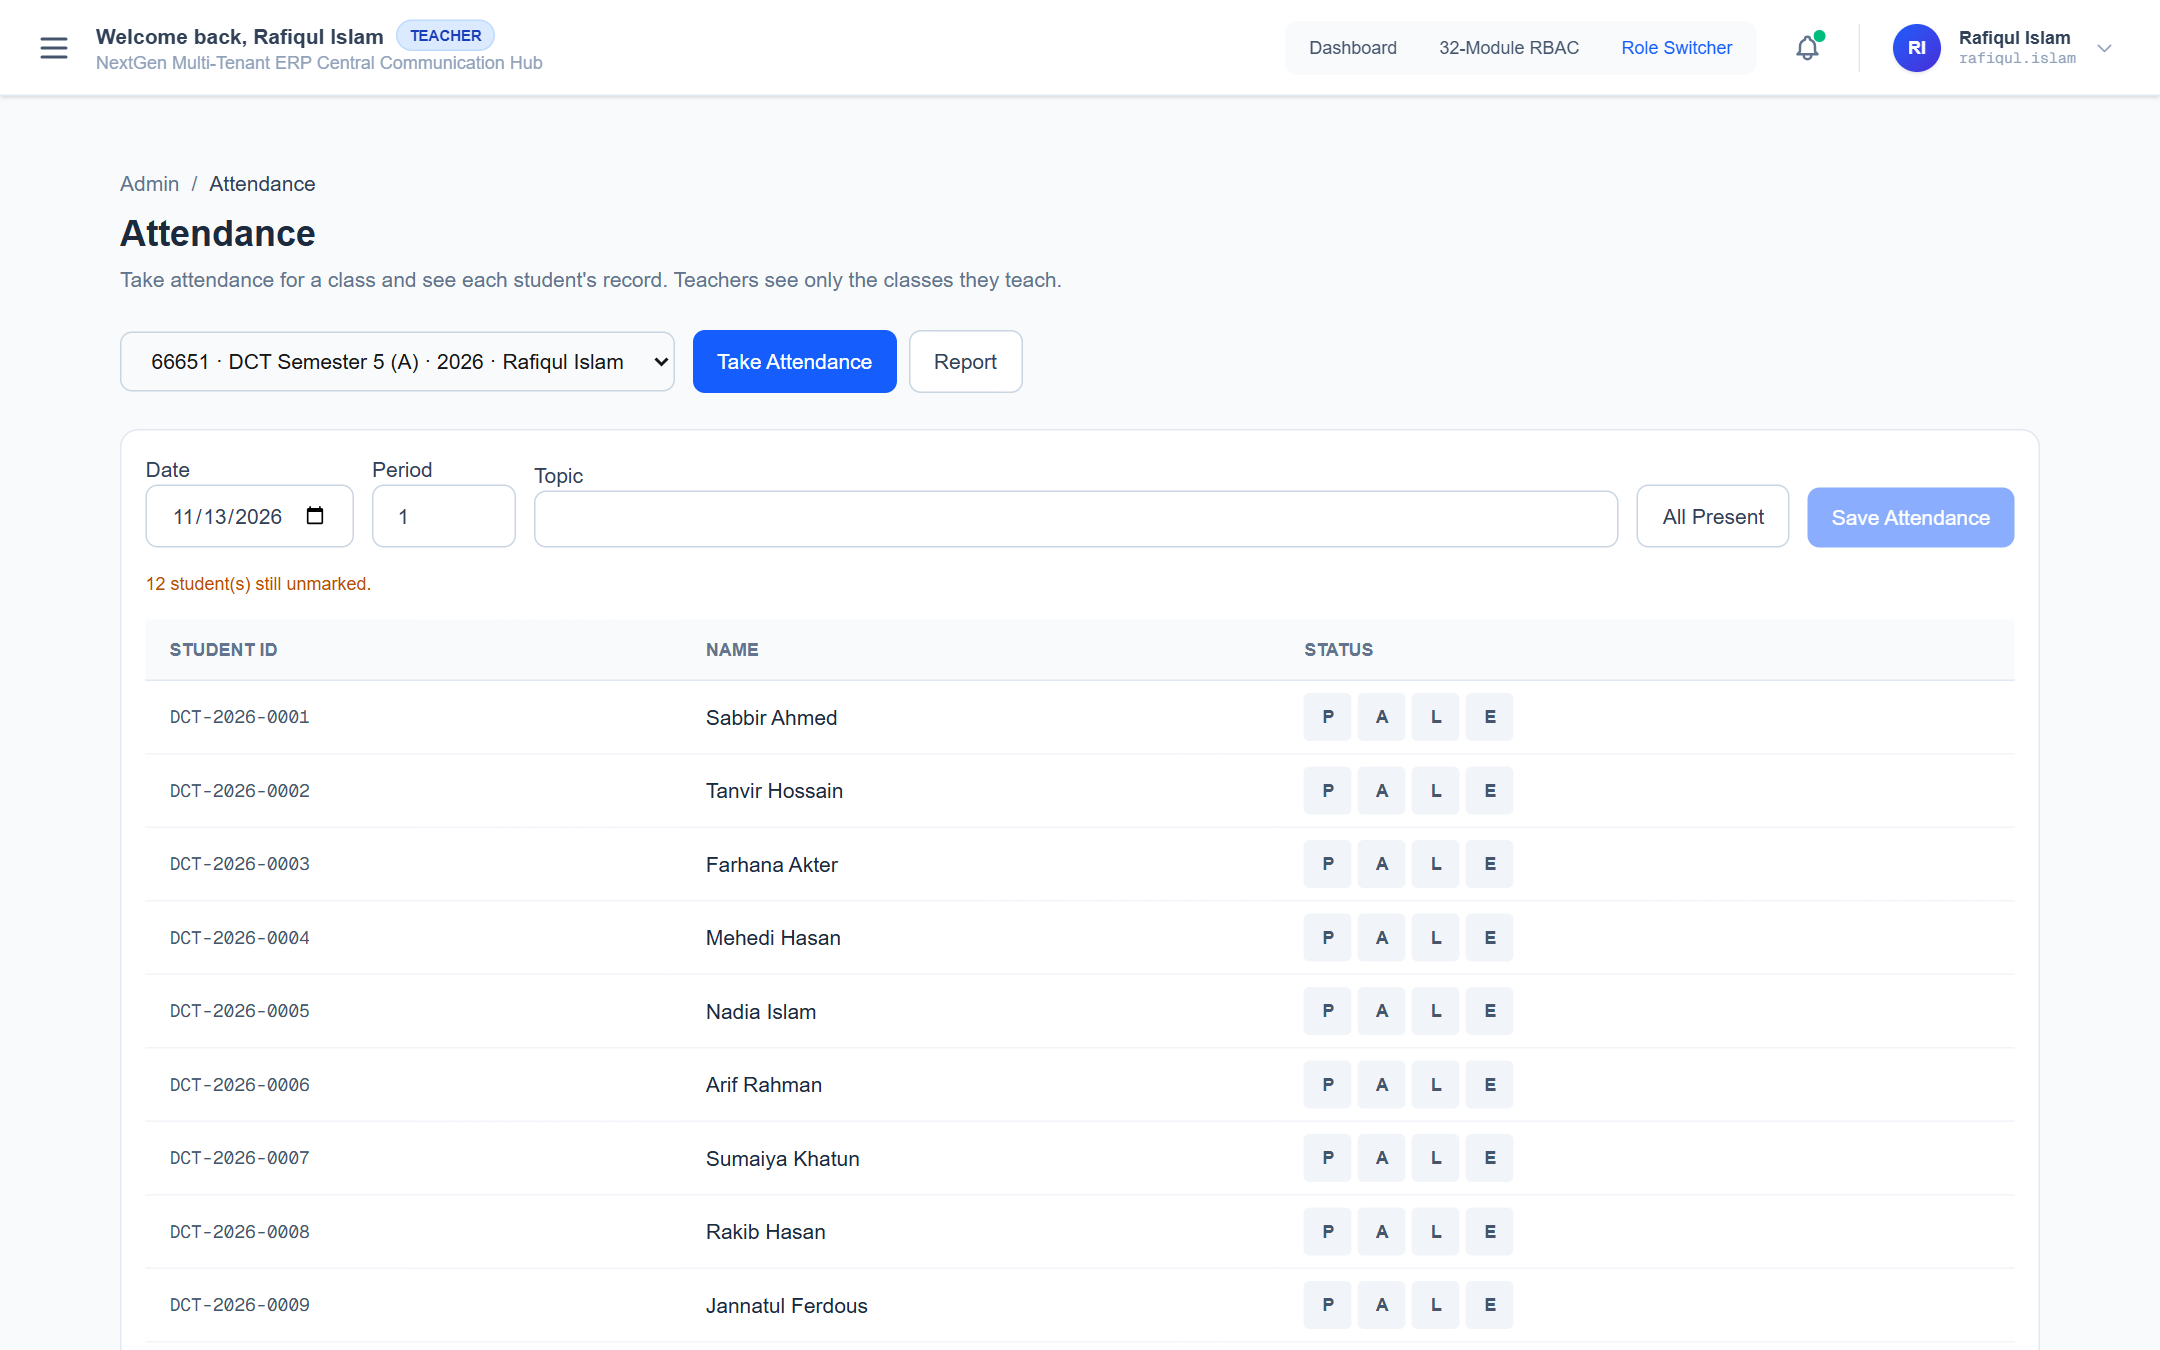
\includegraphics[width=\textwidth]{book_figures/screens/s08_attendance.png}
    \caption{Attendance taken by a teacher}
    \label{fig:impl-attendance}
\end{figure}

Marks are entered on the Marks Entry screen in Figure~\ref{fig:impl-marks}. The teacher chooses a class and an exam assessment, enters each student's marks within the maximum marks or marks the student absent, and locks the assessment when it is complete.

\begin{figure}[H]
    \centering
    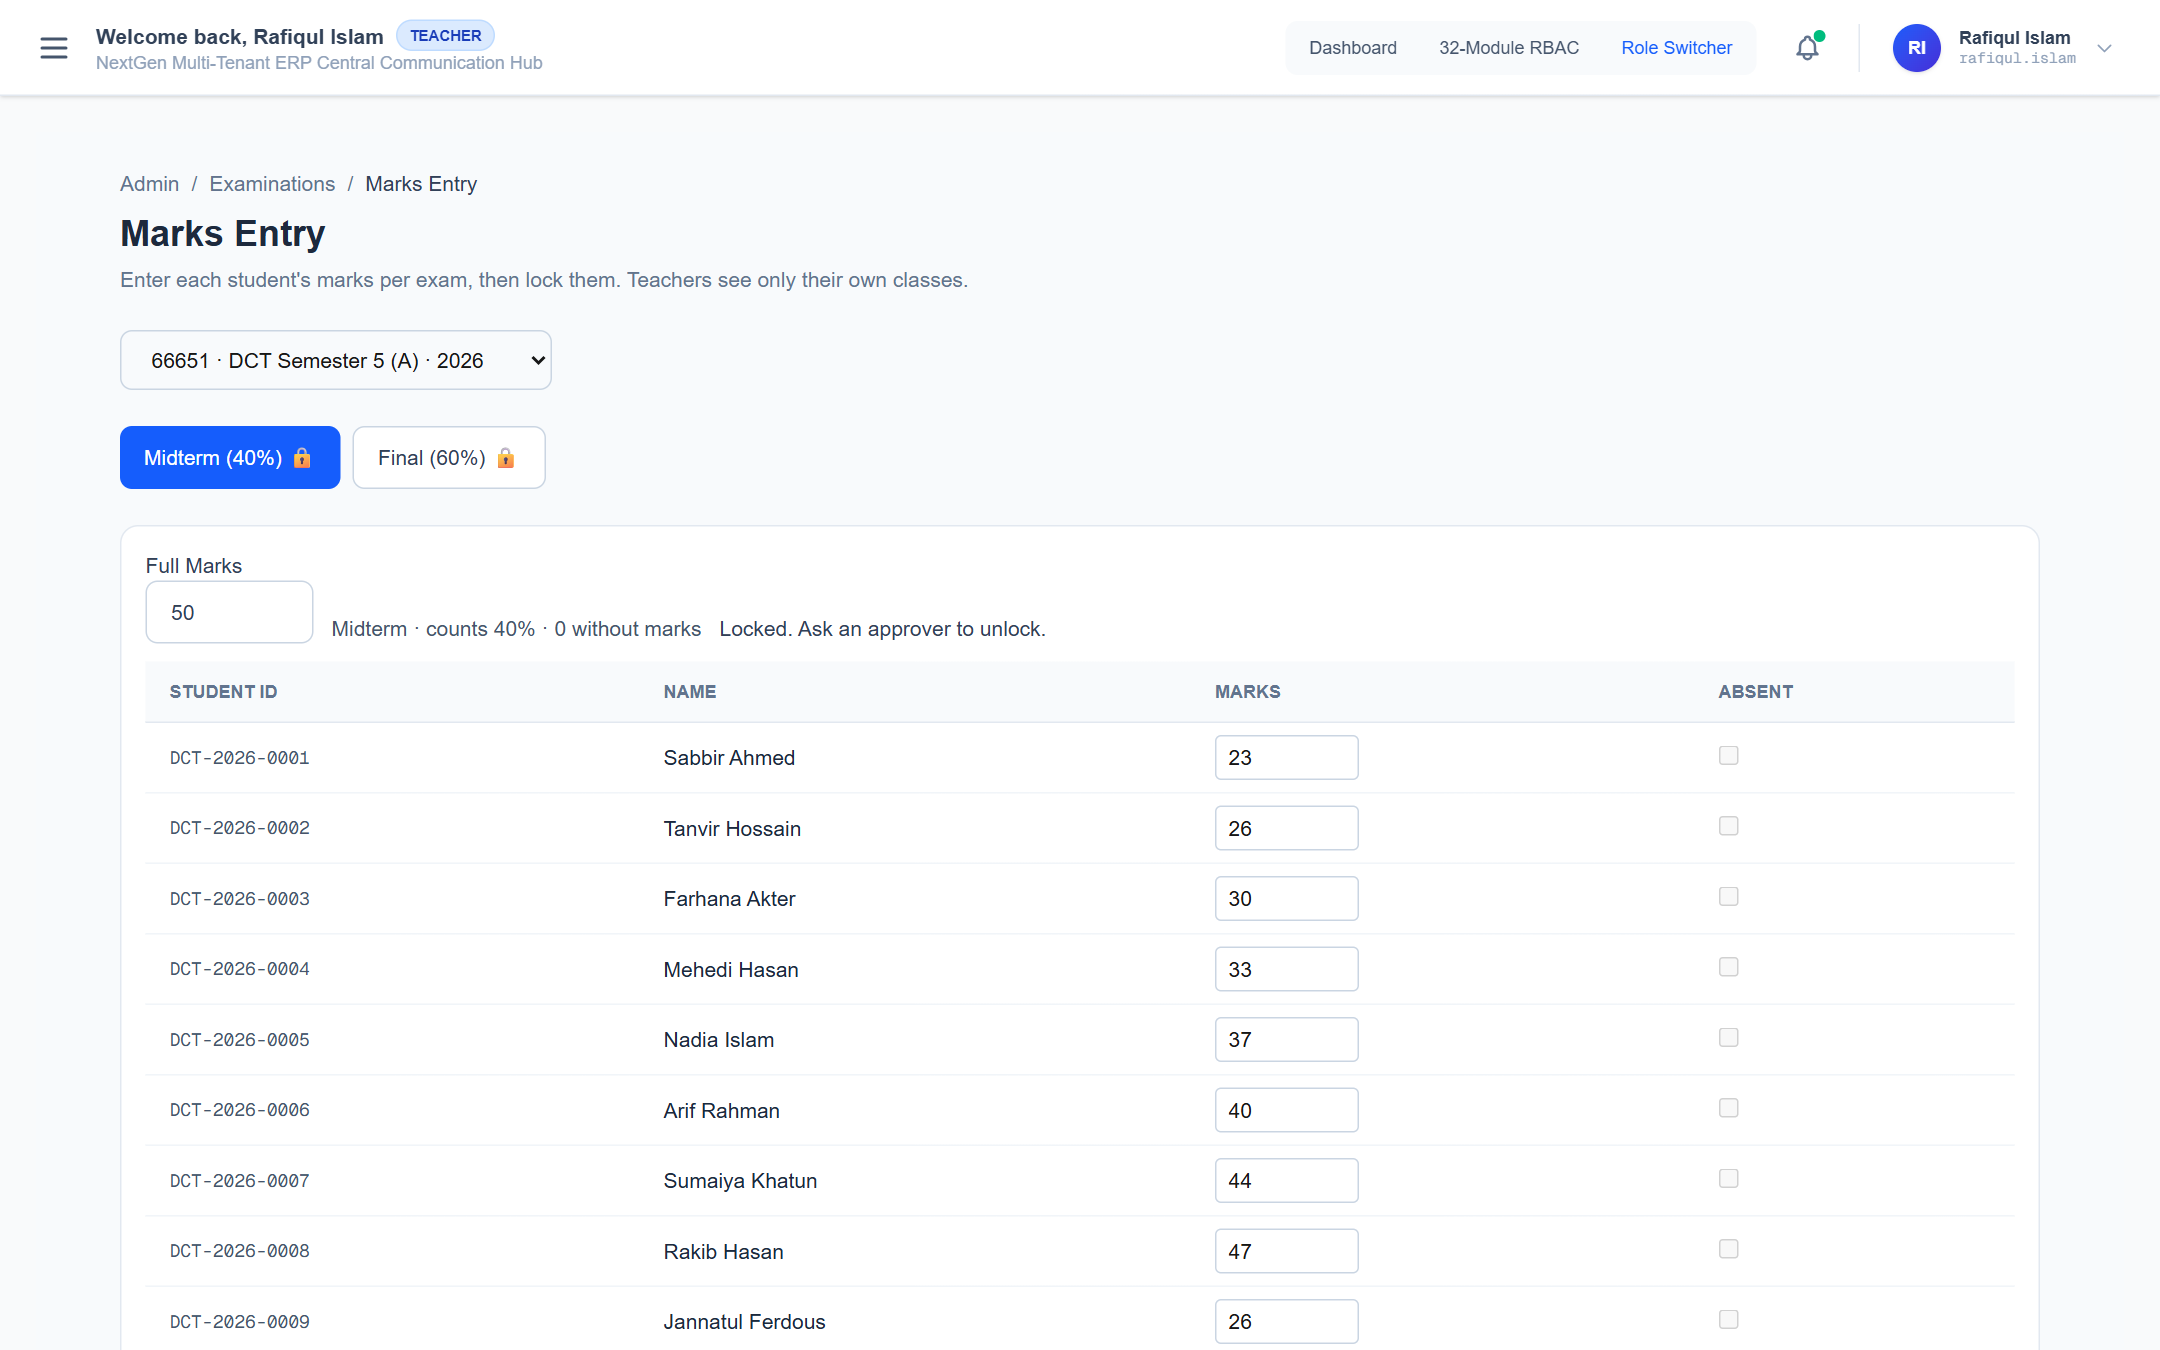
\includegraphics[width=\textwidth]{book_figures/screens/s09_marks_entry.png}
    \caption{Marks entry by a teacher}
    \label{fig:impl-marks}
\end{figure}

The Results screen in Figure~\ref{fig:impl-results} shows, for each student of a class, the marks of each exam, the weighted total percentage, and the letter grade, grade point and pass or fail from the institution's grading scale. The status line confirms that the exams carry 100\%, all marks are locked and the results were published; an administrator can also withdraw them.

\begin{figure}[H]
    \centering
    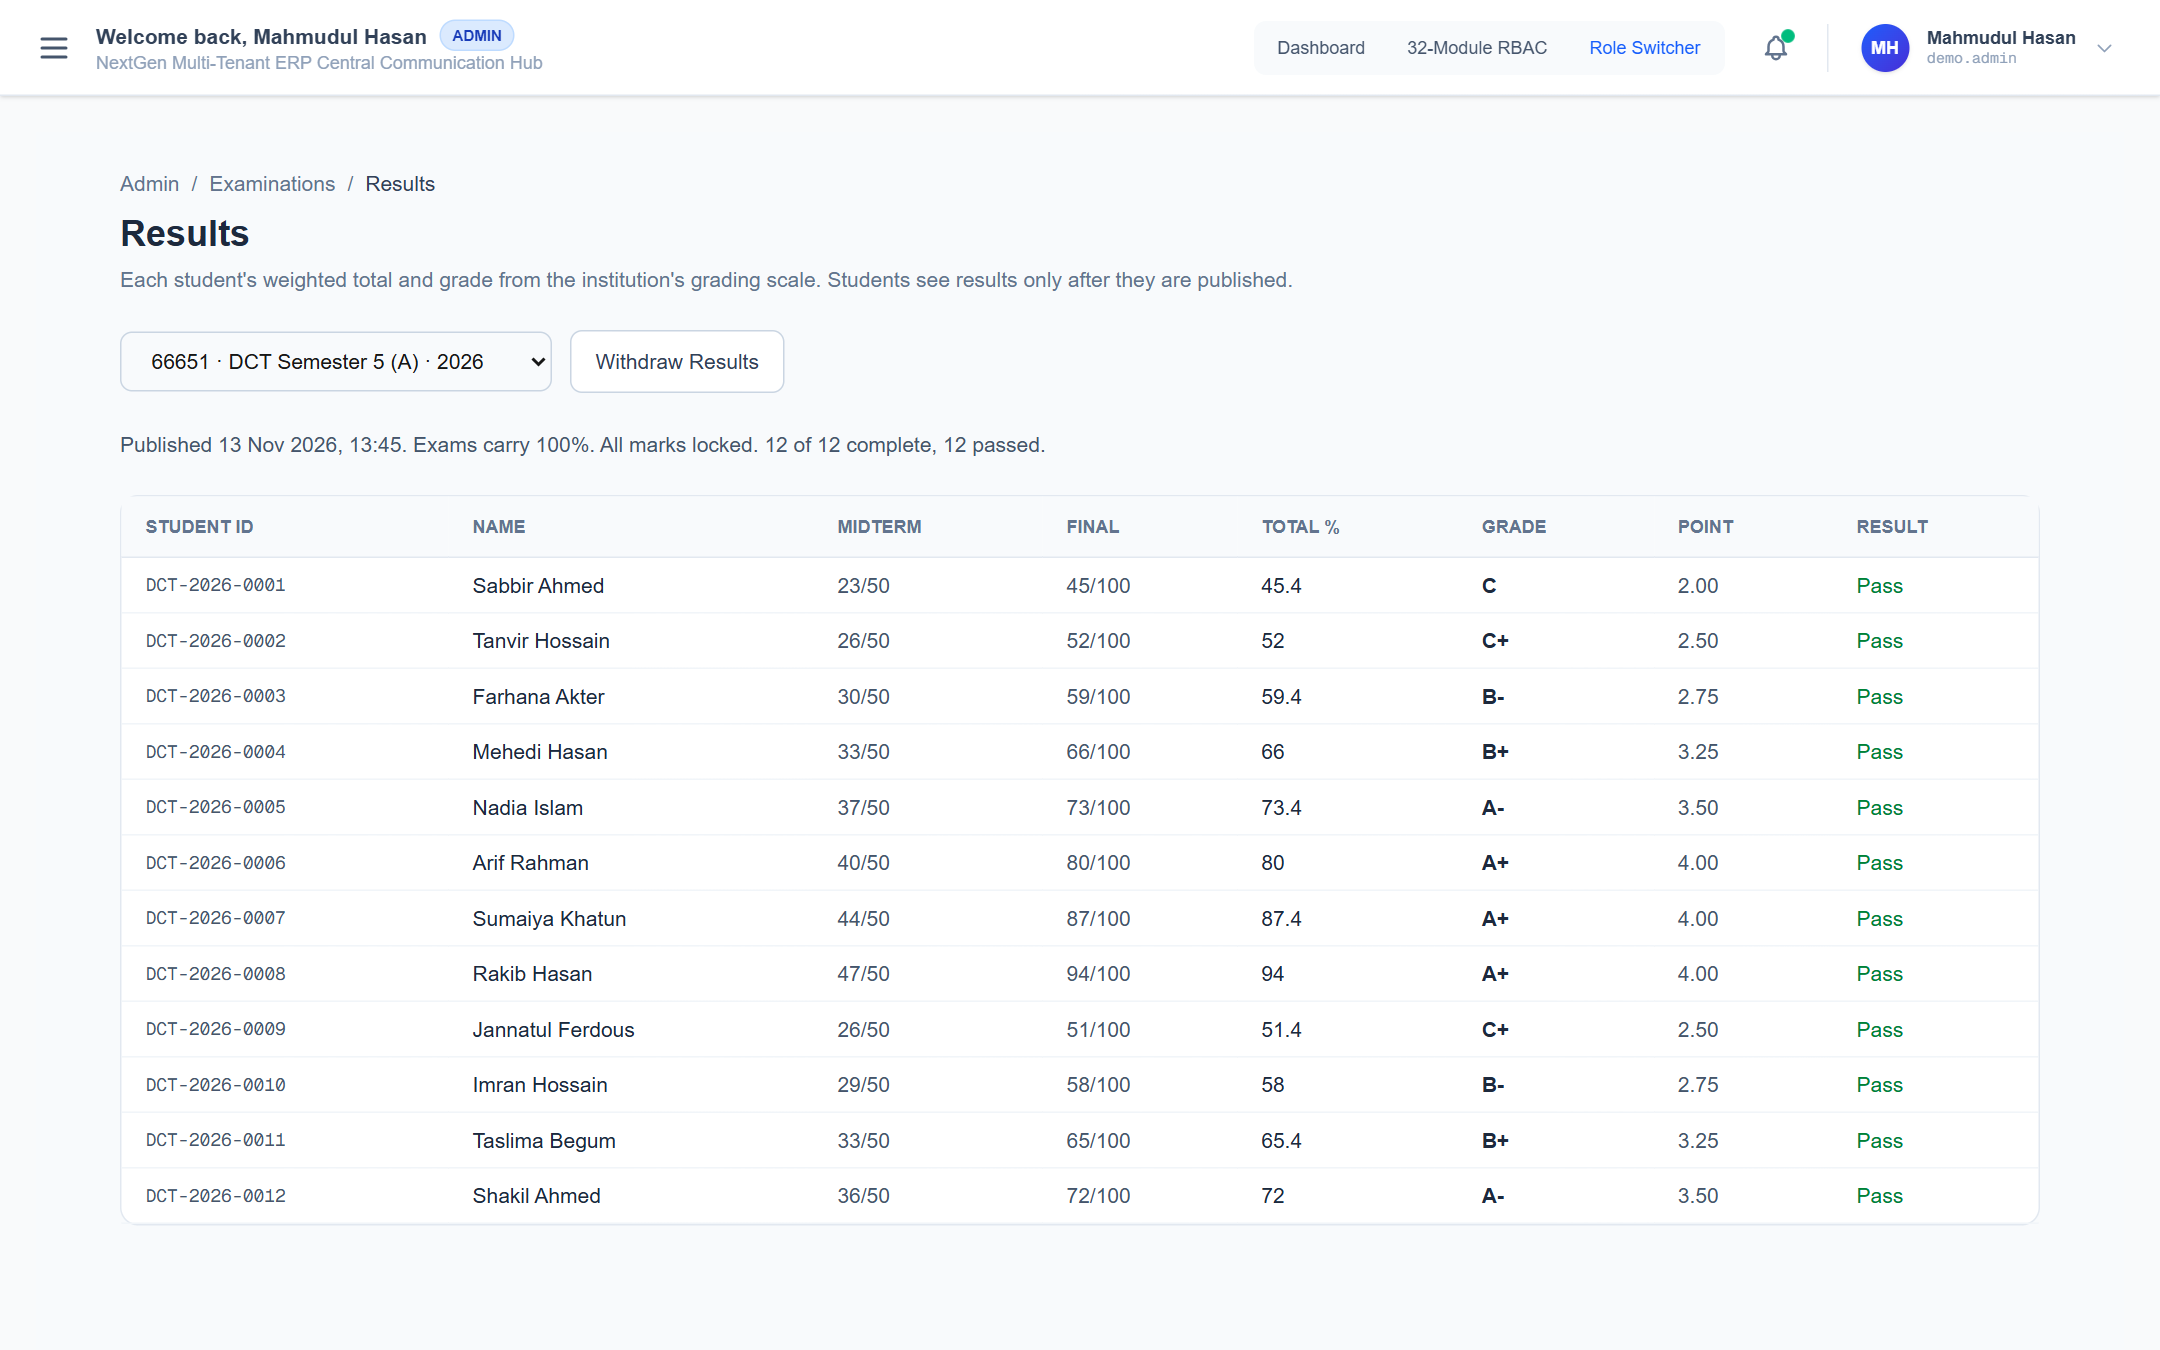
\includegraphics[width=\textwidth]{book_figures/screens/s10_results.png}
    \caption{Class results}
    \label{fig:impl-results}
\end{figure}

\section{Finance and Billing}
The Invoices screen in Figure~\ref{fig:impl-invoices} lists student fee invoices with their amounts, paid amounts, outstanding balances, due dates and status. In the demonstration, one batch of semester invoices was generated for the whole program from the fee structure in a single action. Invoices can also be created one by one, adjusted or cancelled with a reason.

\begin{figure}[H]
    \centering
    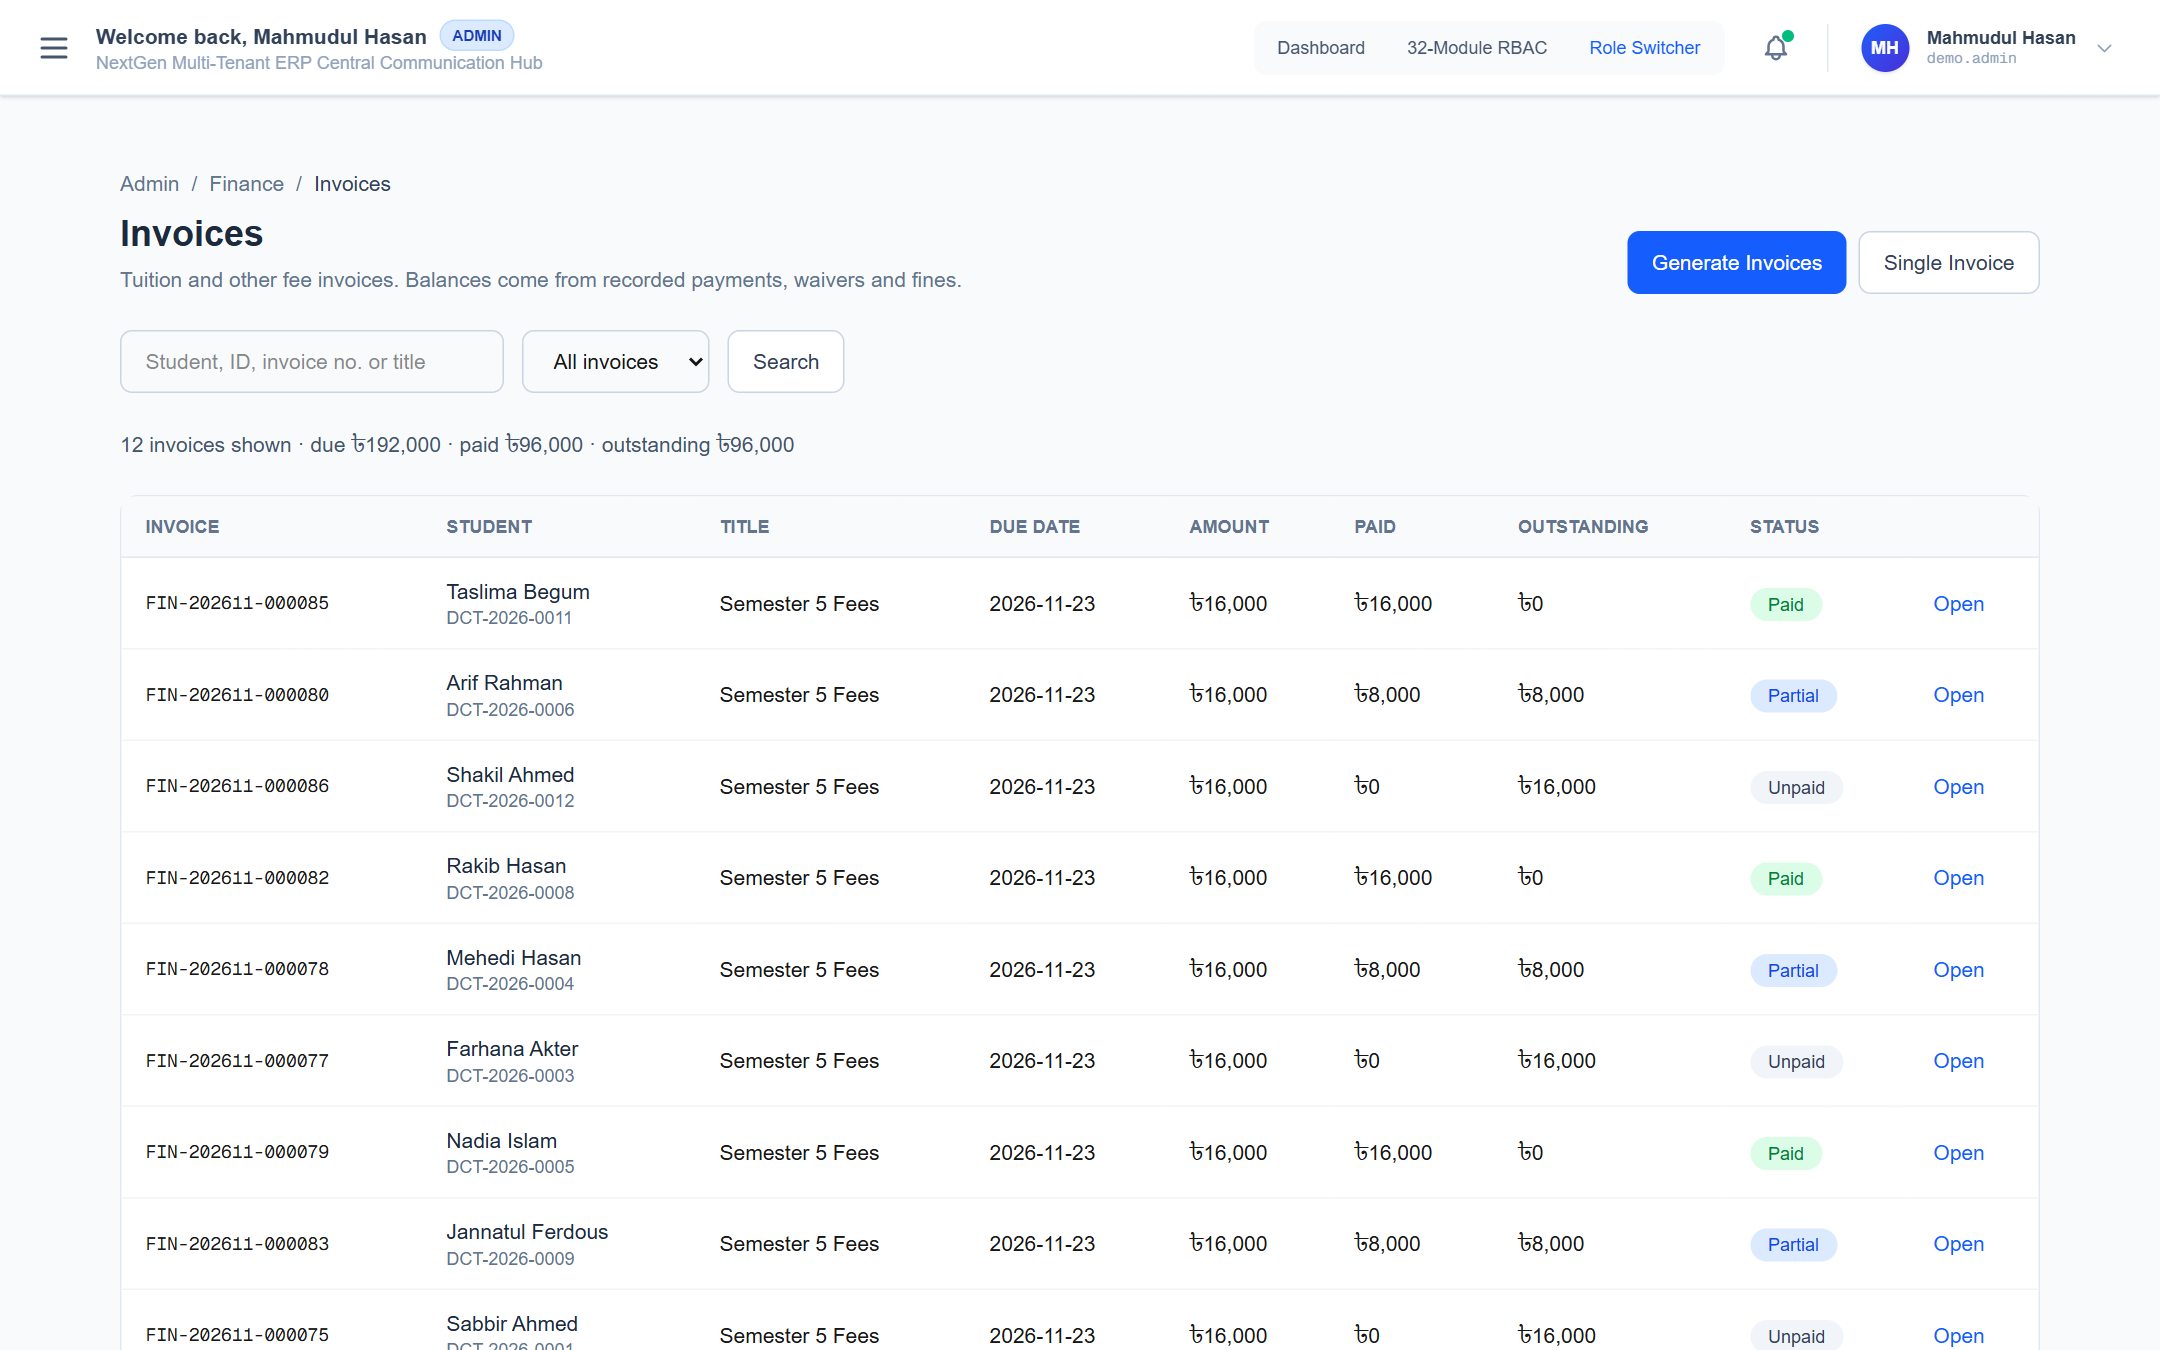
\includegraphics[width=\textwidth]{book_figures/screens/s11_finance_invoices.png}
    \caption{Fee invoices}
    \label{fig:impl-invoices}
\end{figure}

Payments are recorded on the Collect Payment screen in Figure~\ref{fig:impl-payments}, which lists invoices that still have a balance. A payment records the amount, date, method and reference, and receives a receipt number. The Core API rejects a payment larger than the balance, a future date, or a non-cash payment without a reference, and an idempotency key prevents the same payment from being recorded twice.

\begin{figure}[H]
    \centering
    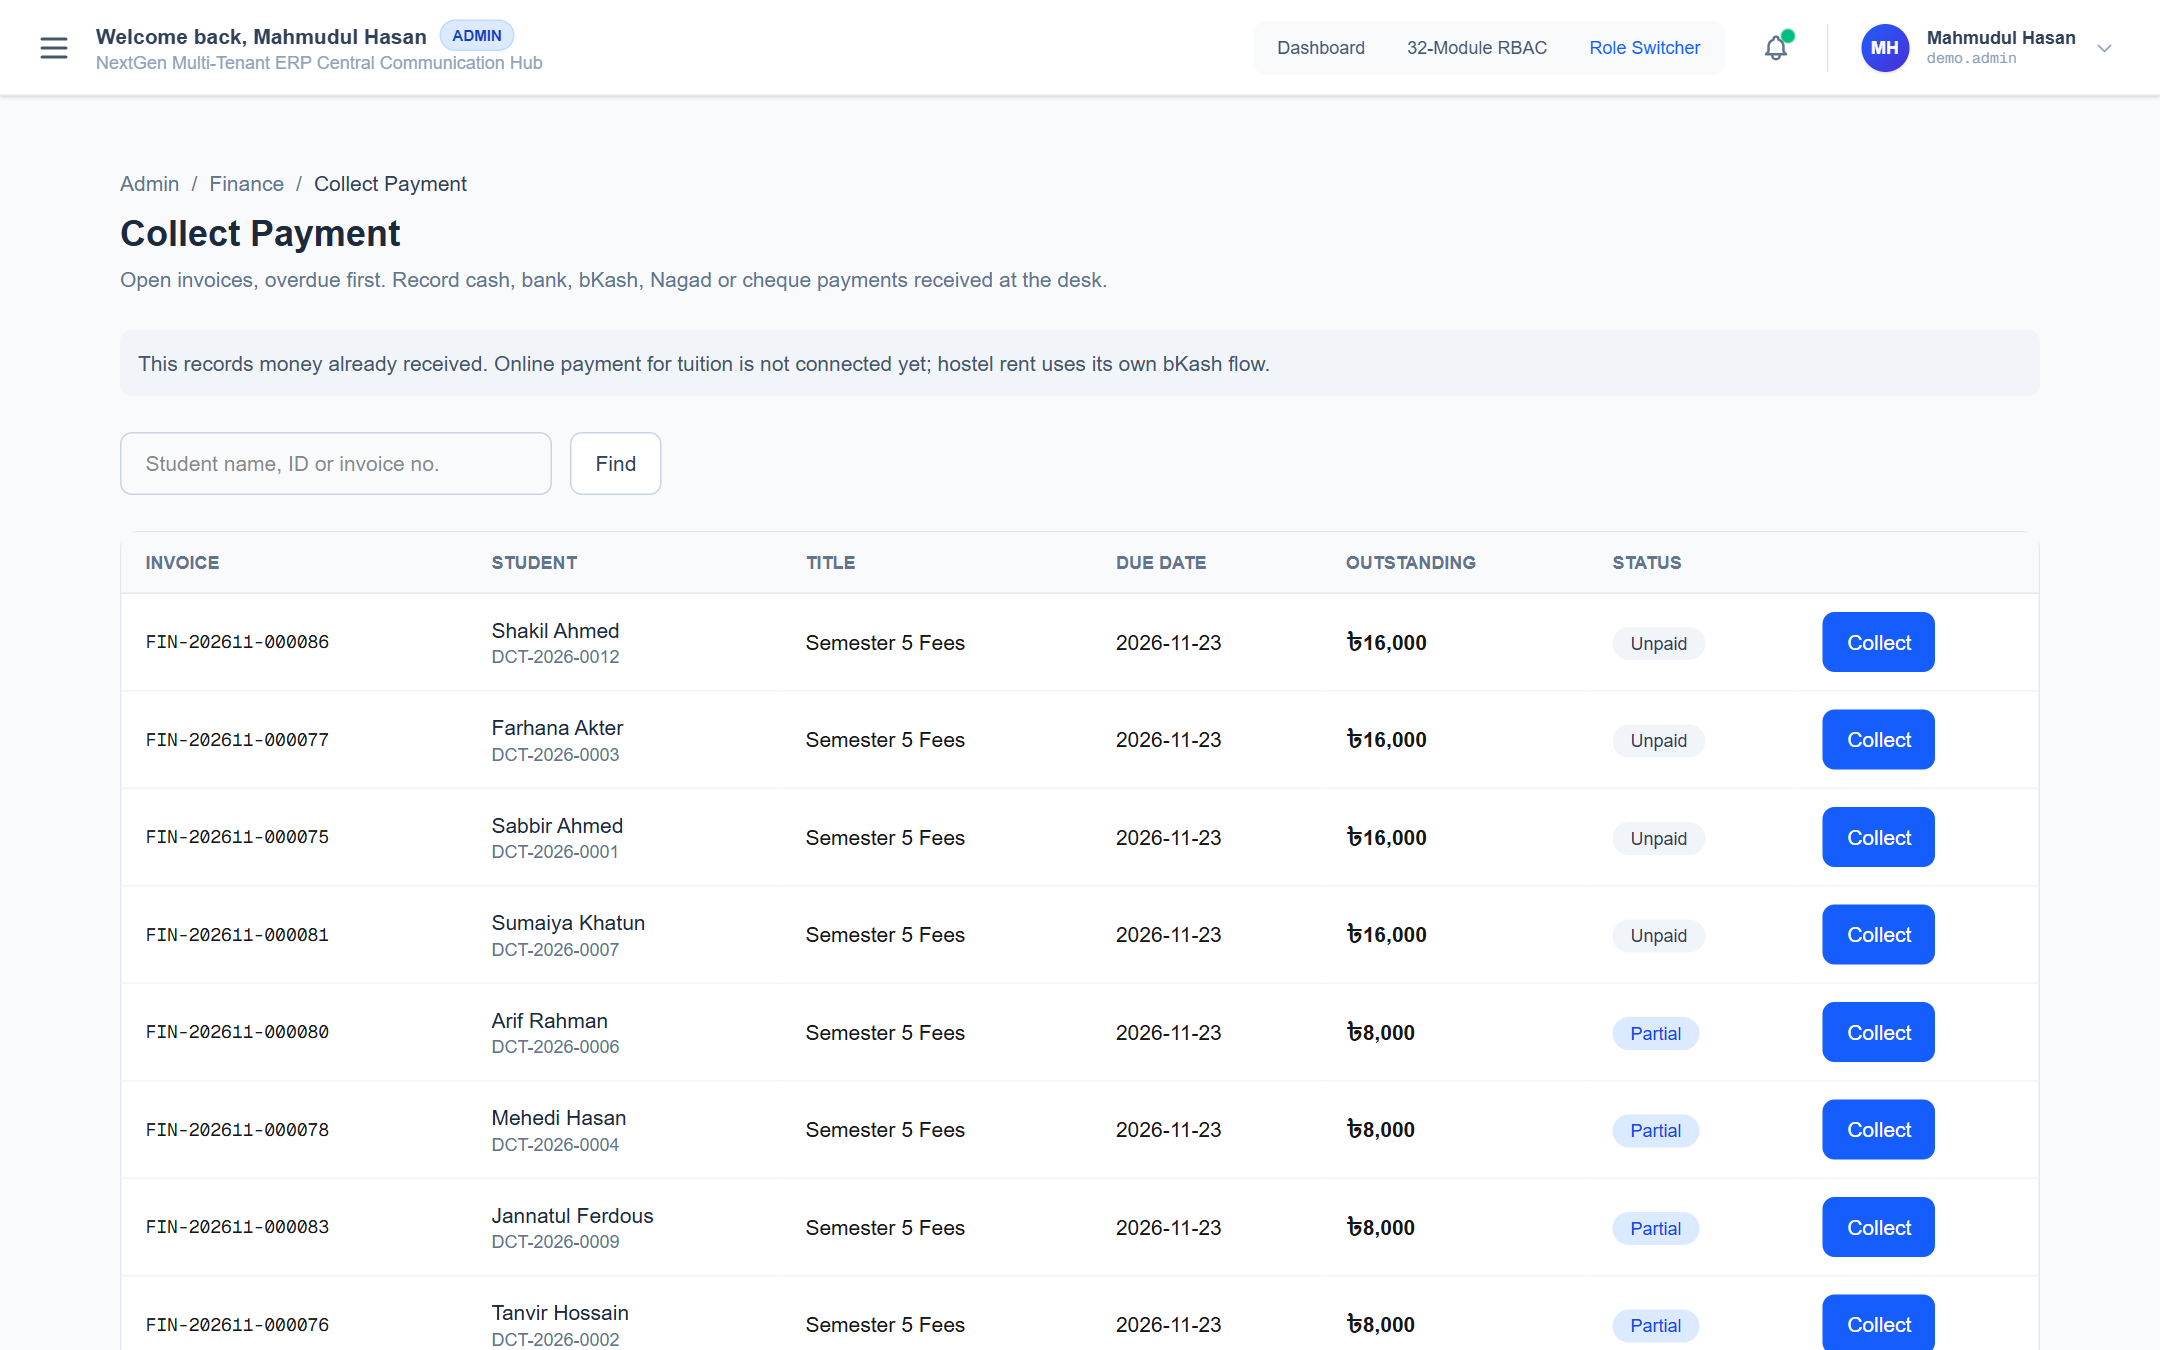
\includegraphics[width=\textwidth]{book_figures/screens/s12_finance_payments.png}
    \caption{Payment collection}
    \label{fig:impl-payments}
\end{figure}

\section{Hostel Management}
The Hostel Control Board in Figure~\ref{fig:impl-hostel} summarises rooms, seats, occupancy and pending applications, together with the rent position of the selected month. It is the starting point for allocations, rent invoices, payments, meals, visitors, maintenance and notifications.

\begin{figure}[H]
    \centering
    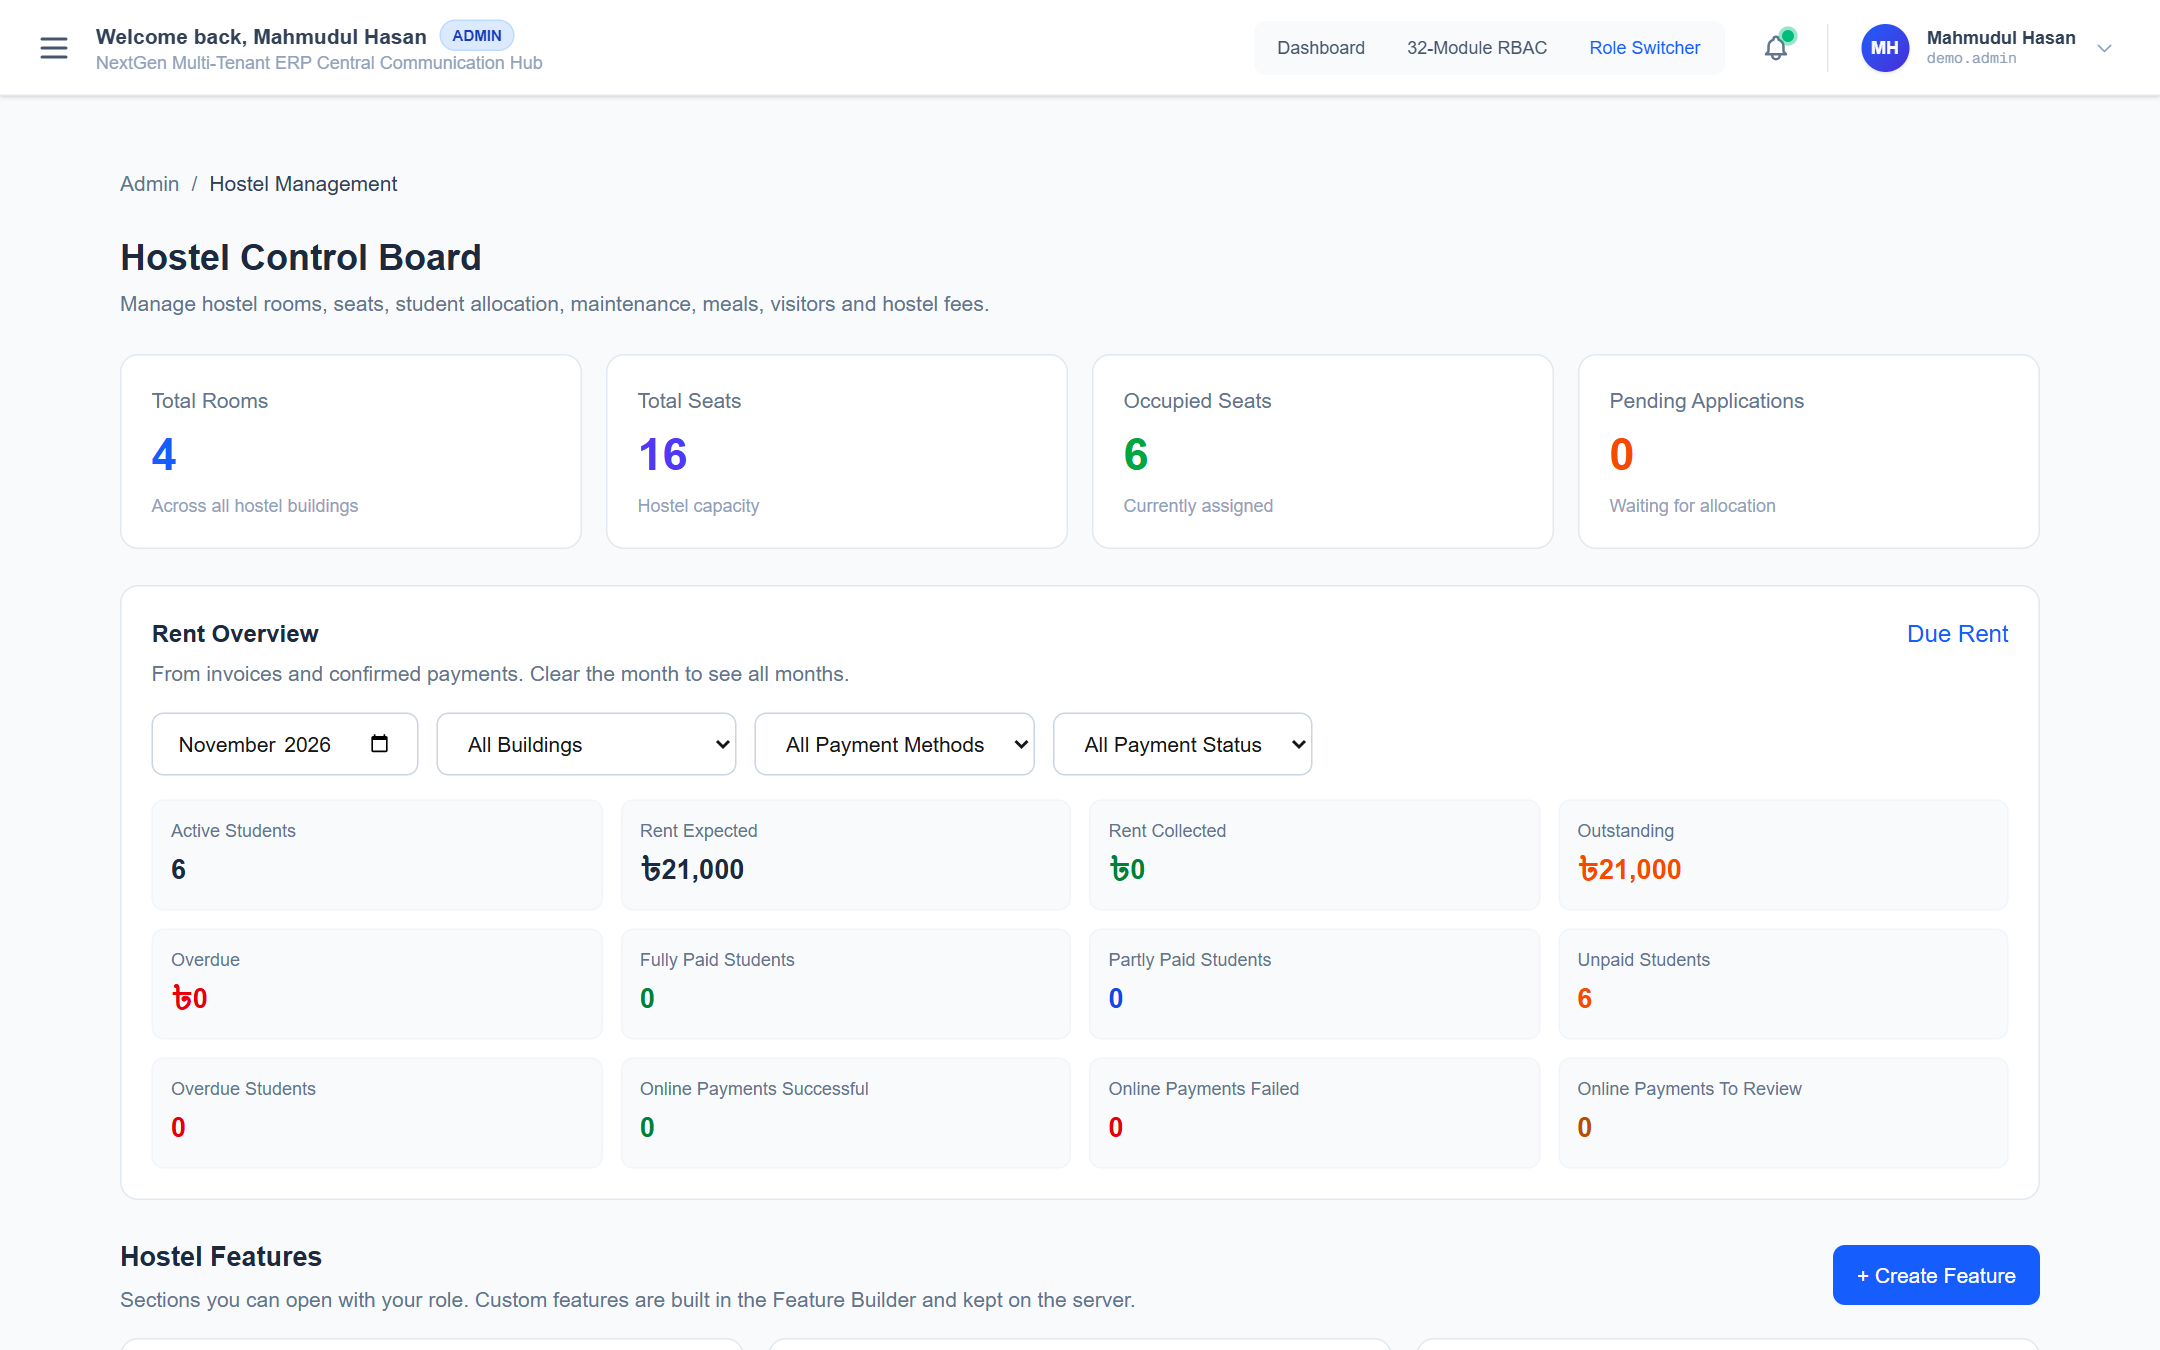
\includegraphics[width=\textwidth]{book_figures/screens/s13_hostel_dashboard.png}
    \caption{Hostel control board}
    \label{fig:impl-hostel}
\end{figure}

The Room Management screen in Figure~\ref{fig:impl-rooms} lists the rooms of each hall with their building, floor, capacity and occupied seats. Rooms can be added one by one or in bulk and exported. Each room is made of seats, and an allocation links a student to one seat, so a seat can never be given to two students at once.

\begin{figure}[H]
    \centering
    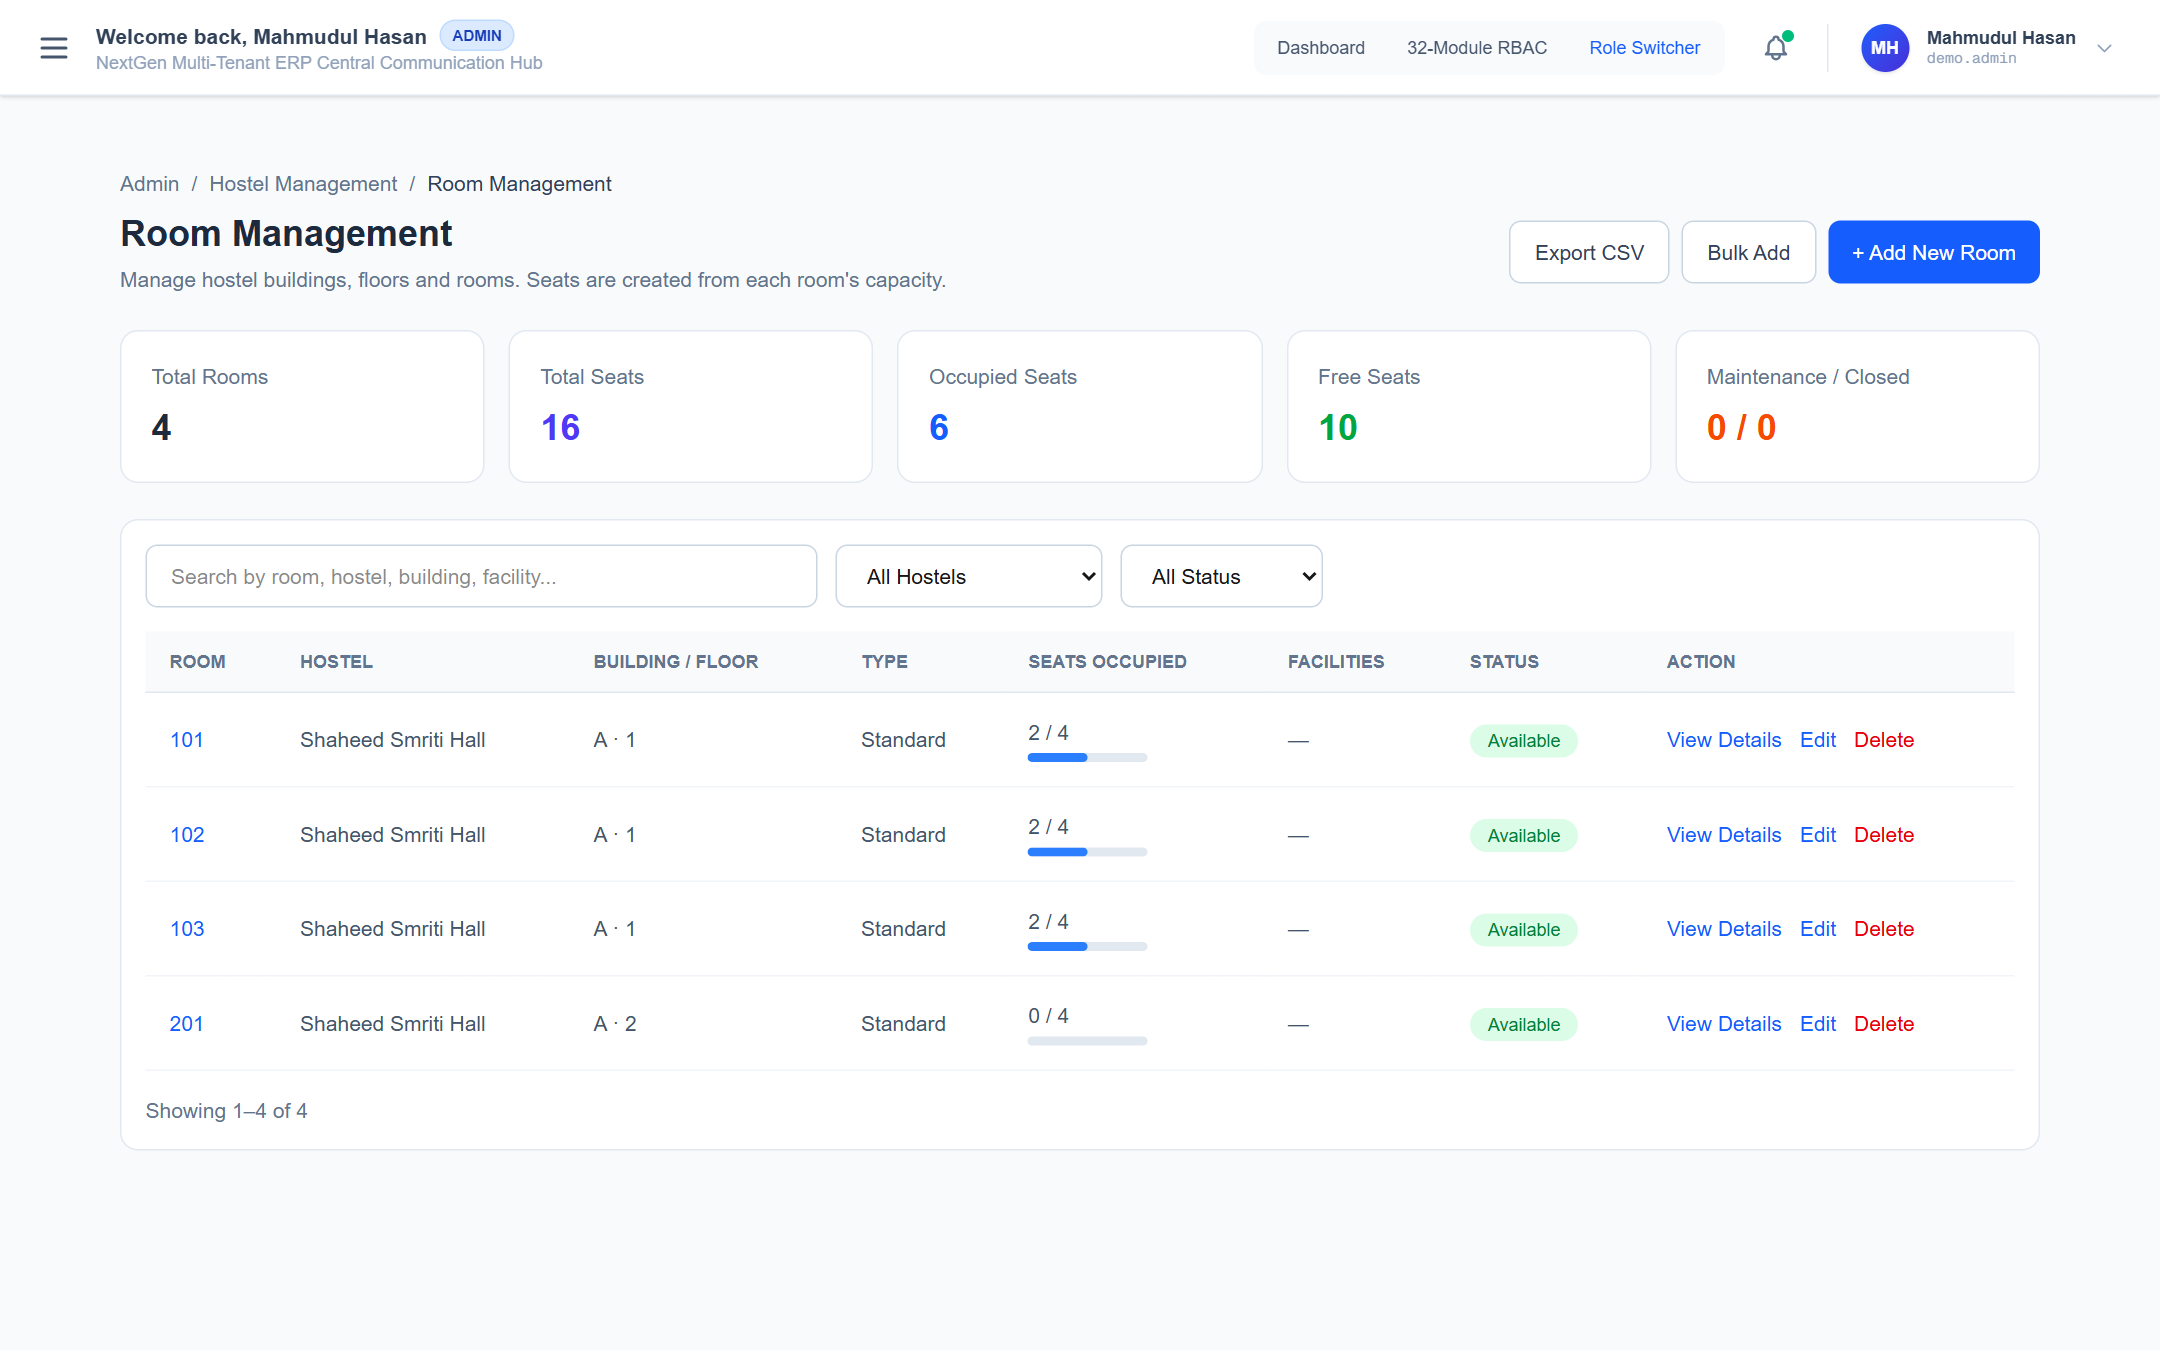
\includegraphics[width=\textwidth]{book_figures/screens/s14_hostel_rooms.png}
    \caption{Hostel room management}
    \label{fig:impl-rooms}
\end{figure}

\section{Library Management}
The Books screen in Figure~\ref{fig:impl-library} holds the catalogue with each book's author, category, total copies and the number of copies available. Library staff issue books to students or teachers, renew loans, record returns and record or waive fines from the loans screen.

\begin{figure}[H]
    \centering
    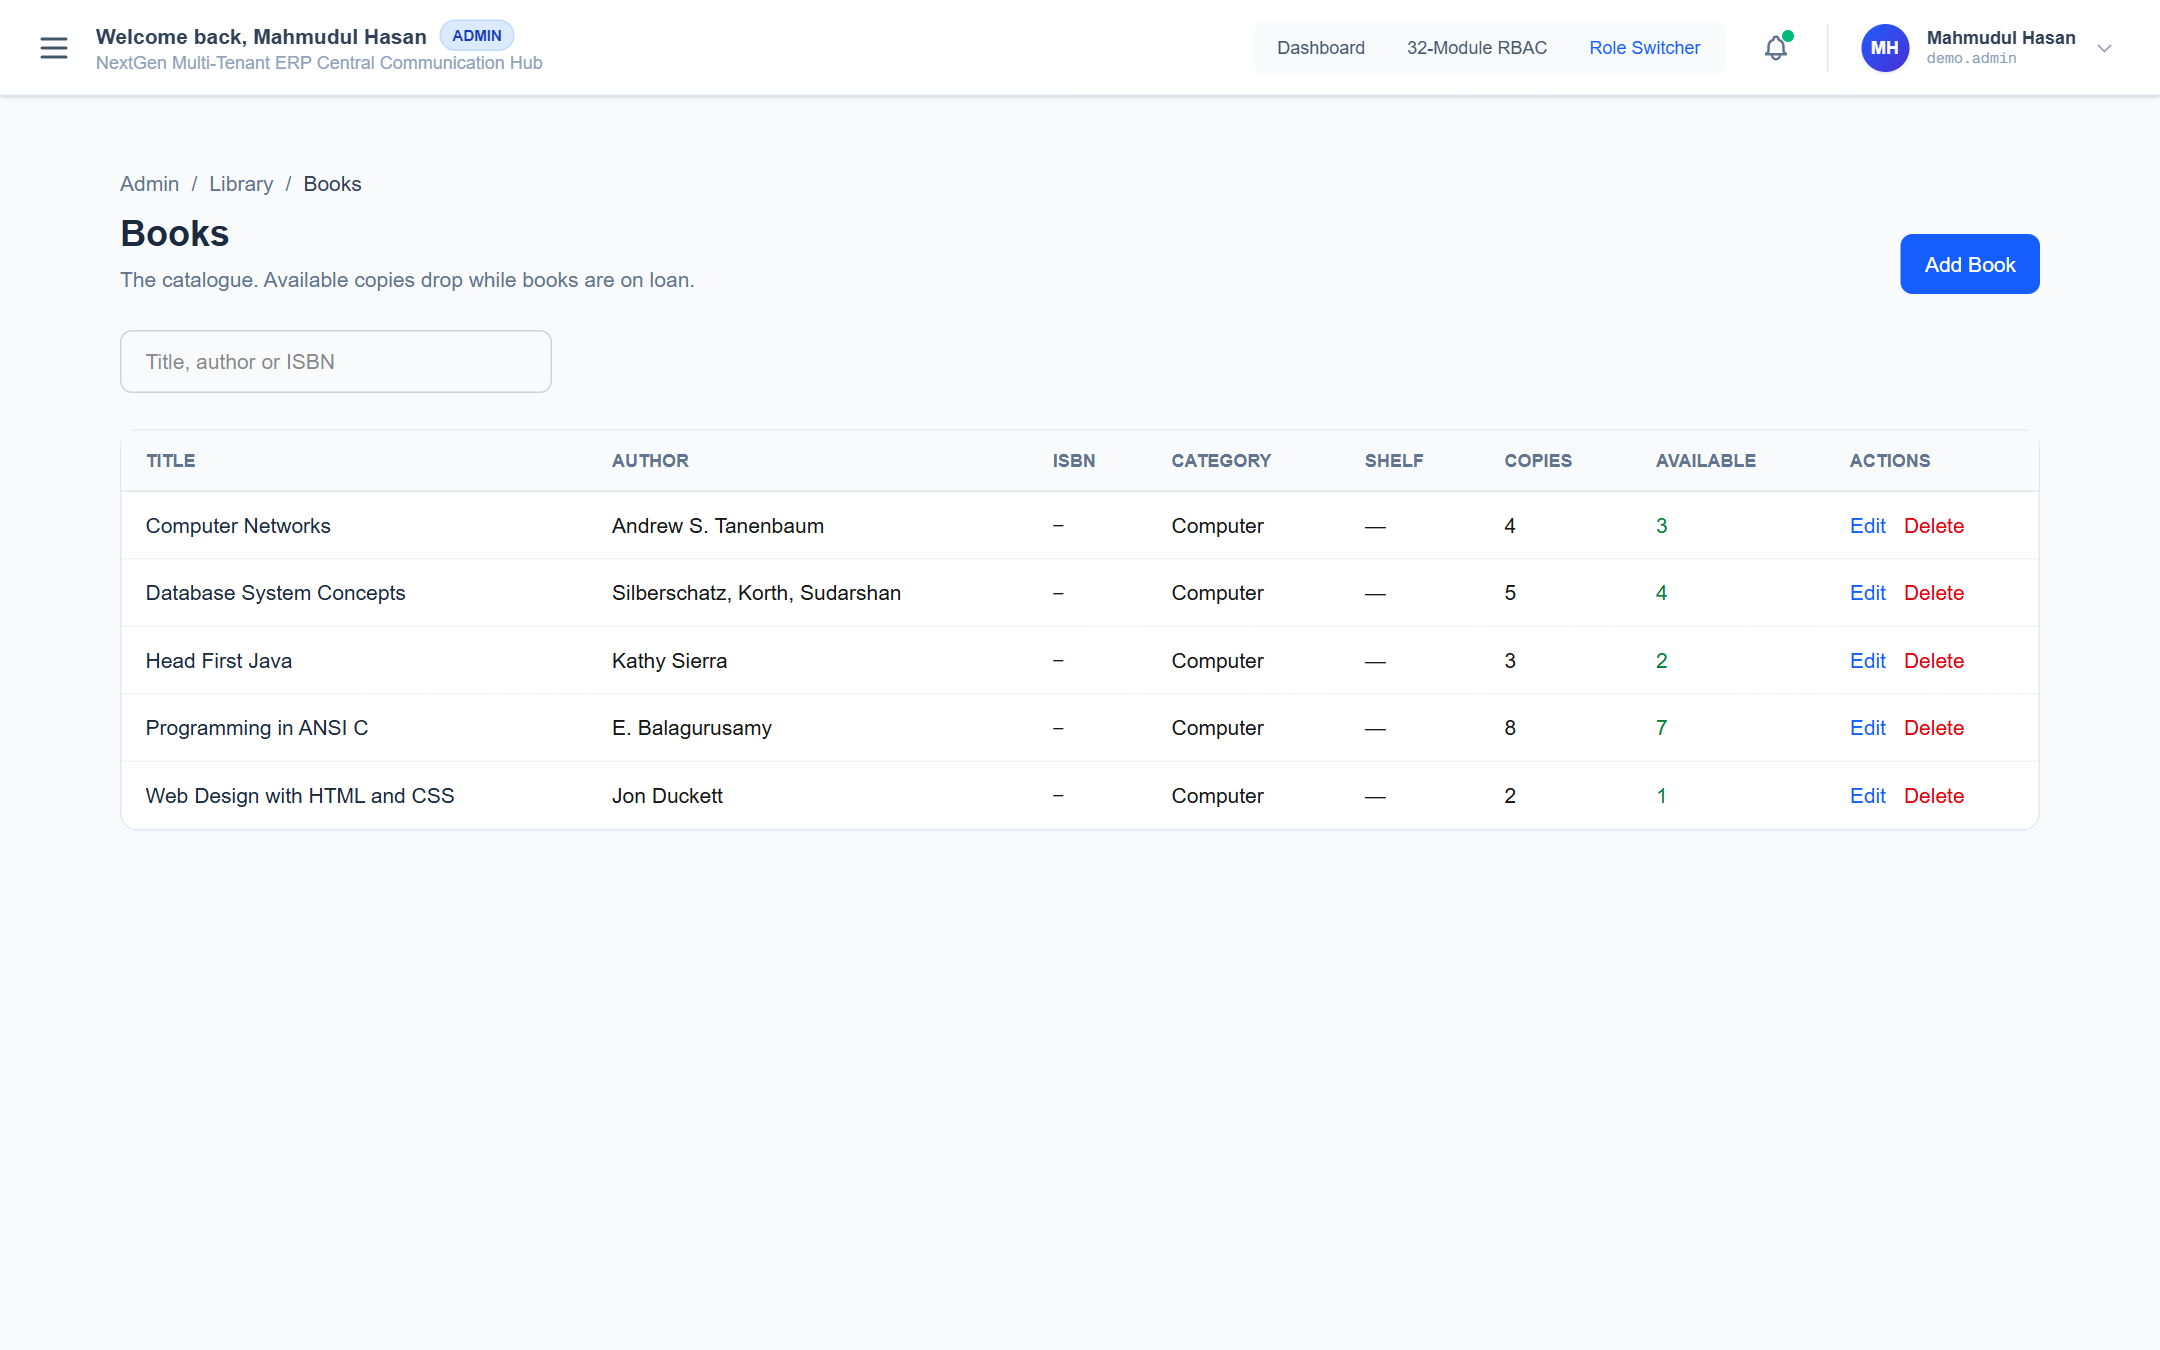
\includegraphics[width=\textwidth]{book_figures/screens/s15_library_books.png}
    \caption{Library catalogue}
    \label{fig:impl-library}
\end{figure}

\section{Human Resources}
The Employees screen in Figure~\ref{fig:impl-hr} lists teachers and other staff together with their designation, department and status. Staff records are added here, while teachers come from the academic module. From this screen, administrators set salaries, and from the related screens they manage leave types, leave requests and payroll runs.

\begin{figure}[H]
    \centering
    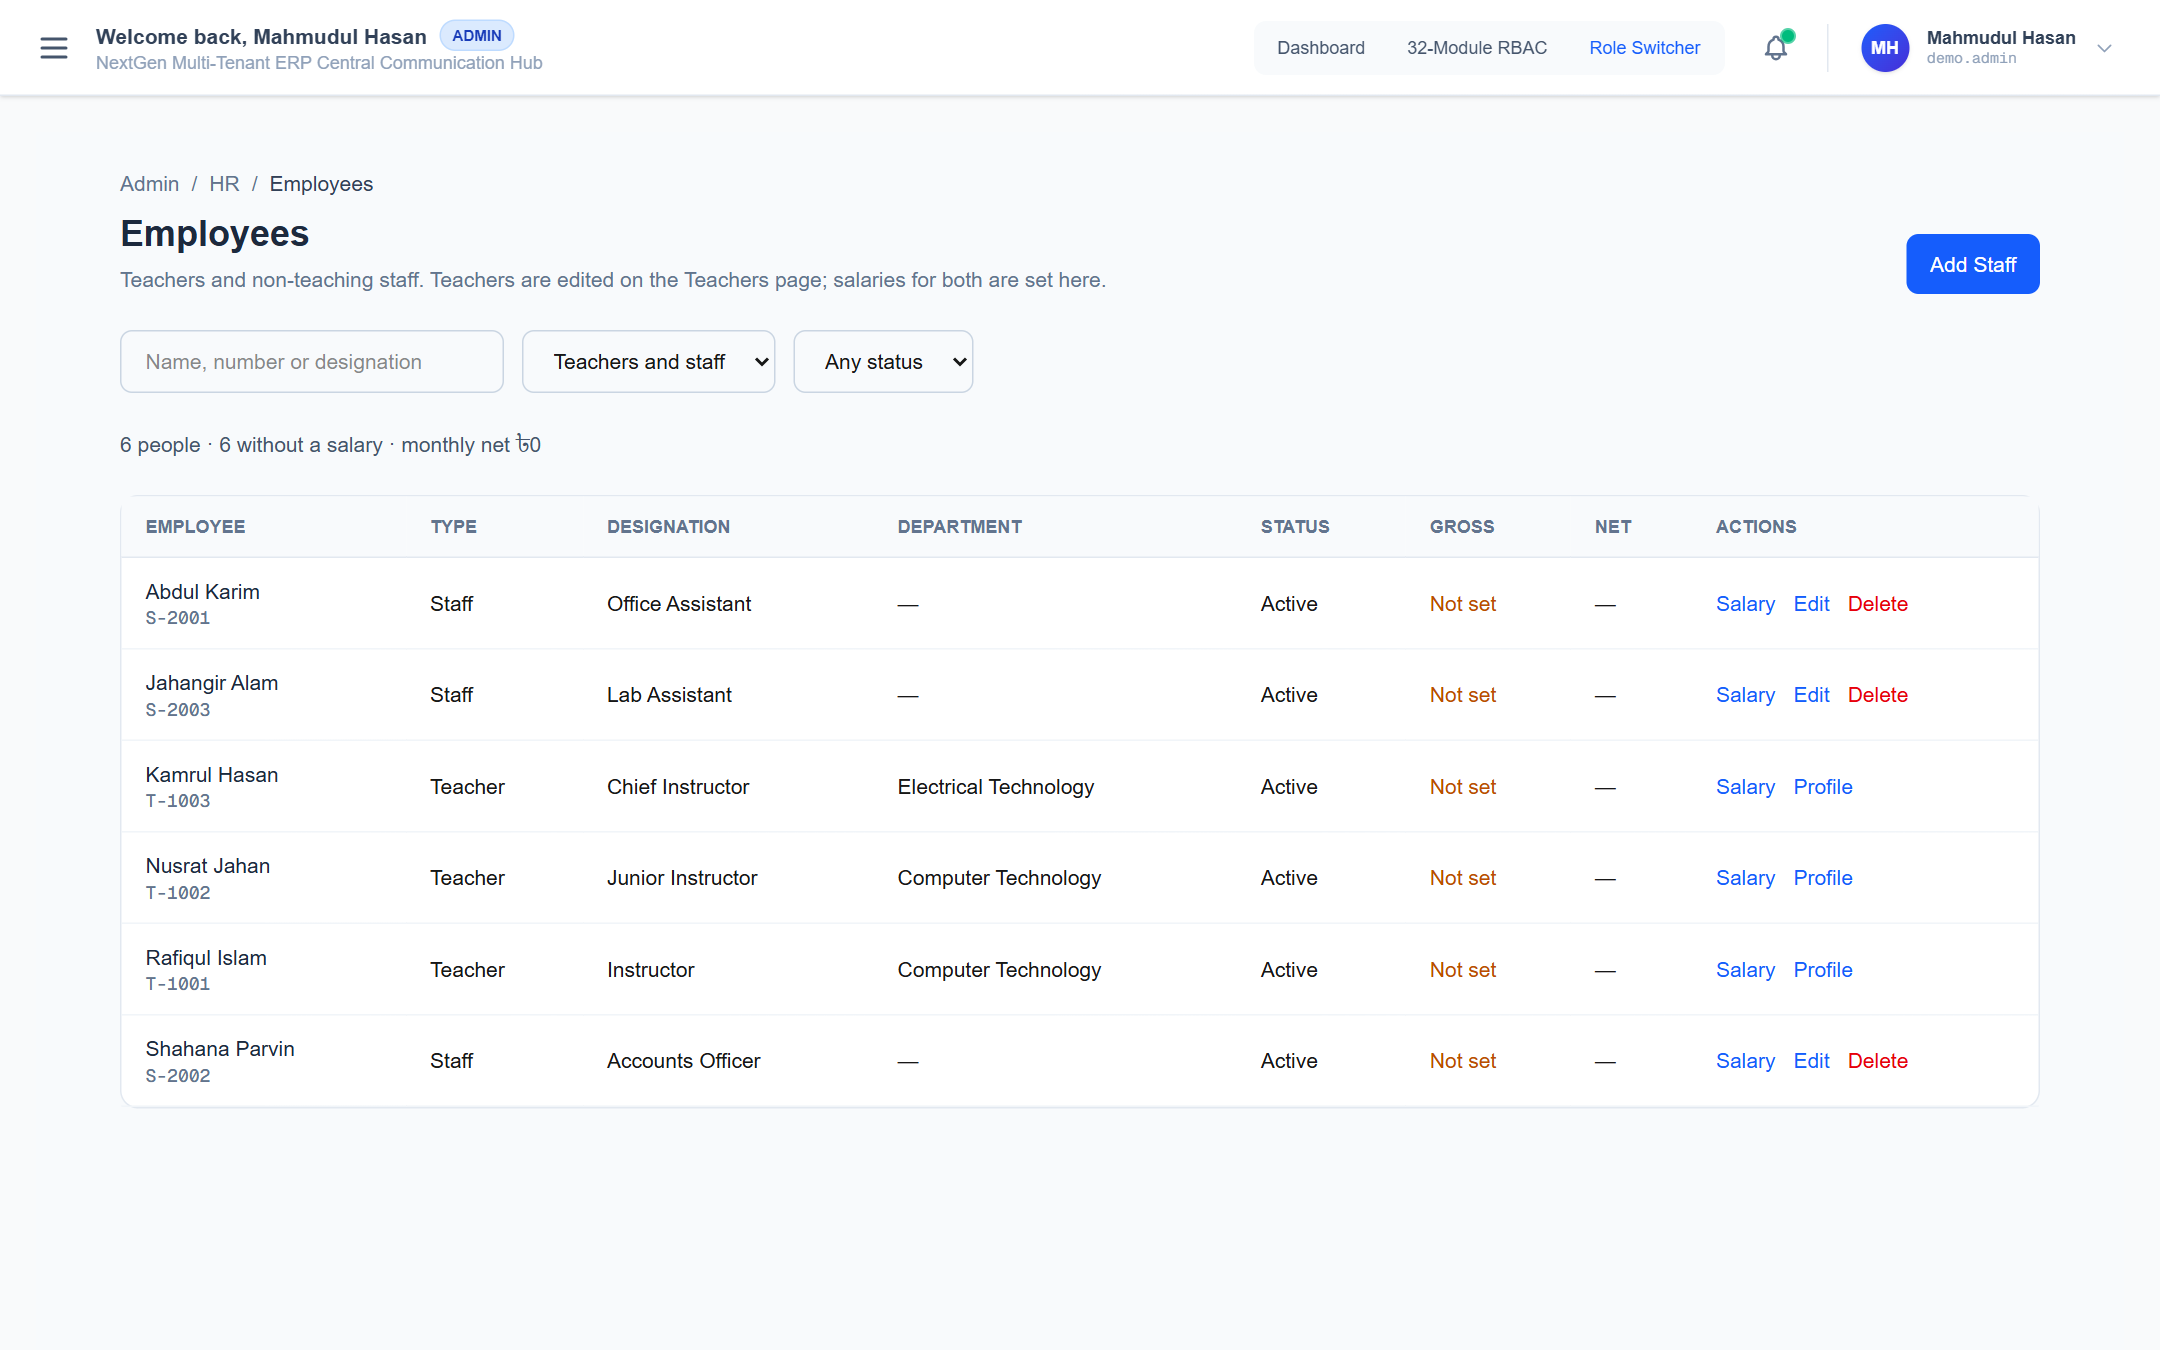
\includegraphics[width=\textwidth]{book_figures/screens/s16_hr_employees.png}
    \caption{Employees}
    \label{fig:impl-hr}
\end{figure}

\section{Inventory Management}
The Items and Stock screen in Figure~\ref{fig:impl-inventory} lists stock items with their category, quantity on hand, reorder level and stock value, and marks items that are low. In the demonstration, items were received into the main store from a supplier invoice in one receipt. Items can also be imported from a file and exported. Every receipt, issue, return, count, write-off and transfer is recorded as a stock movement.

\begin{figure}[H]
    \centering
    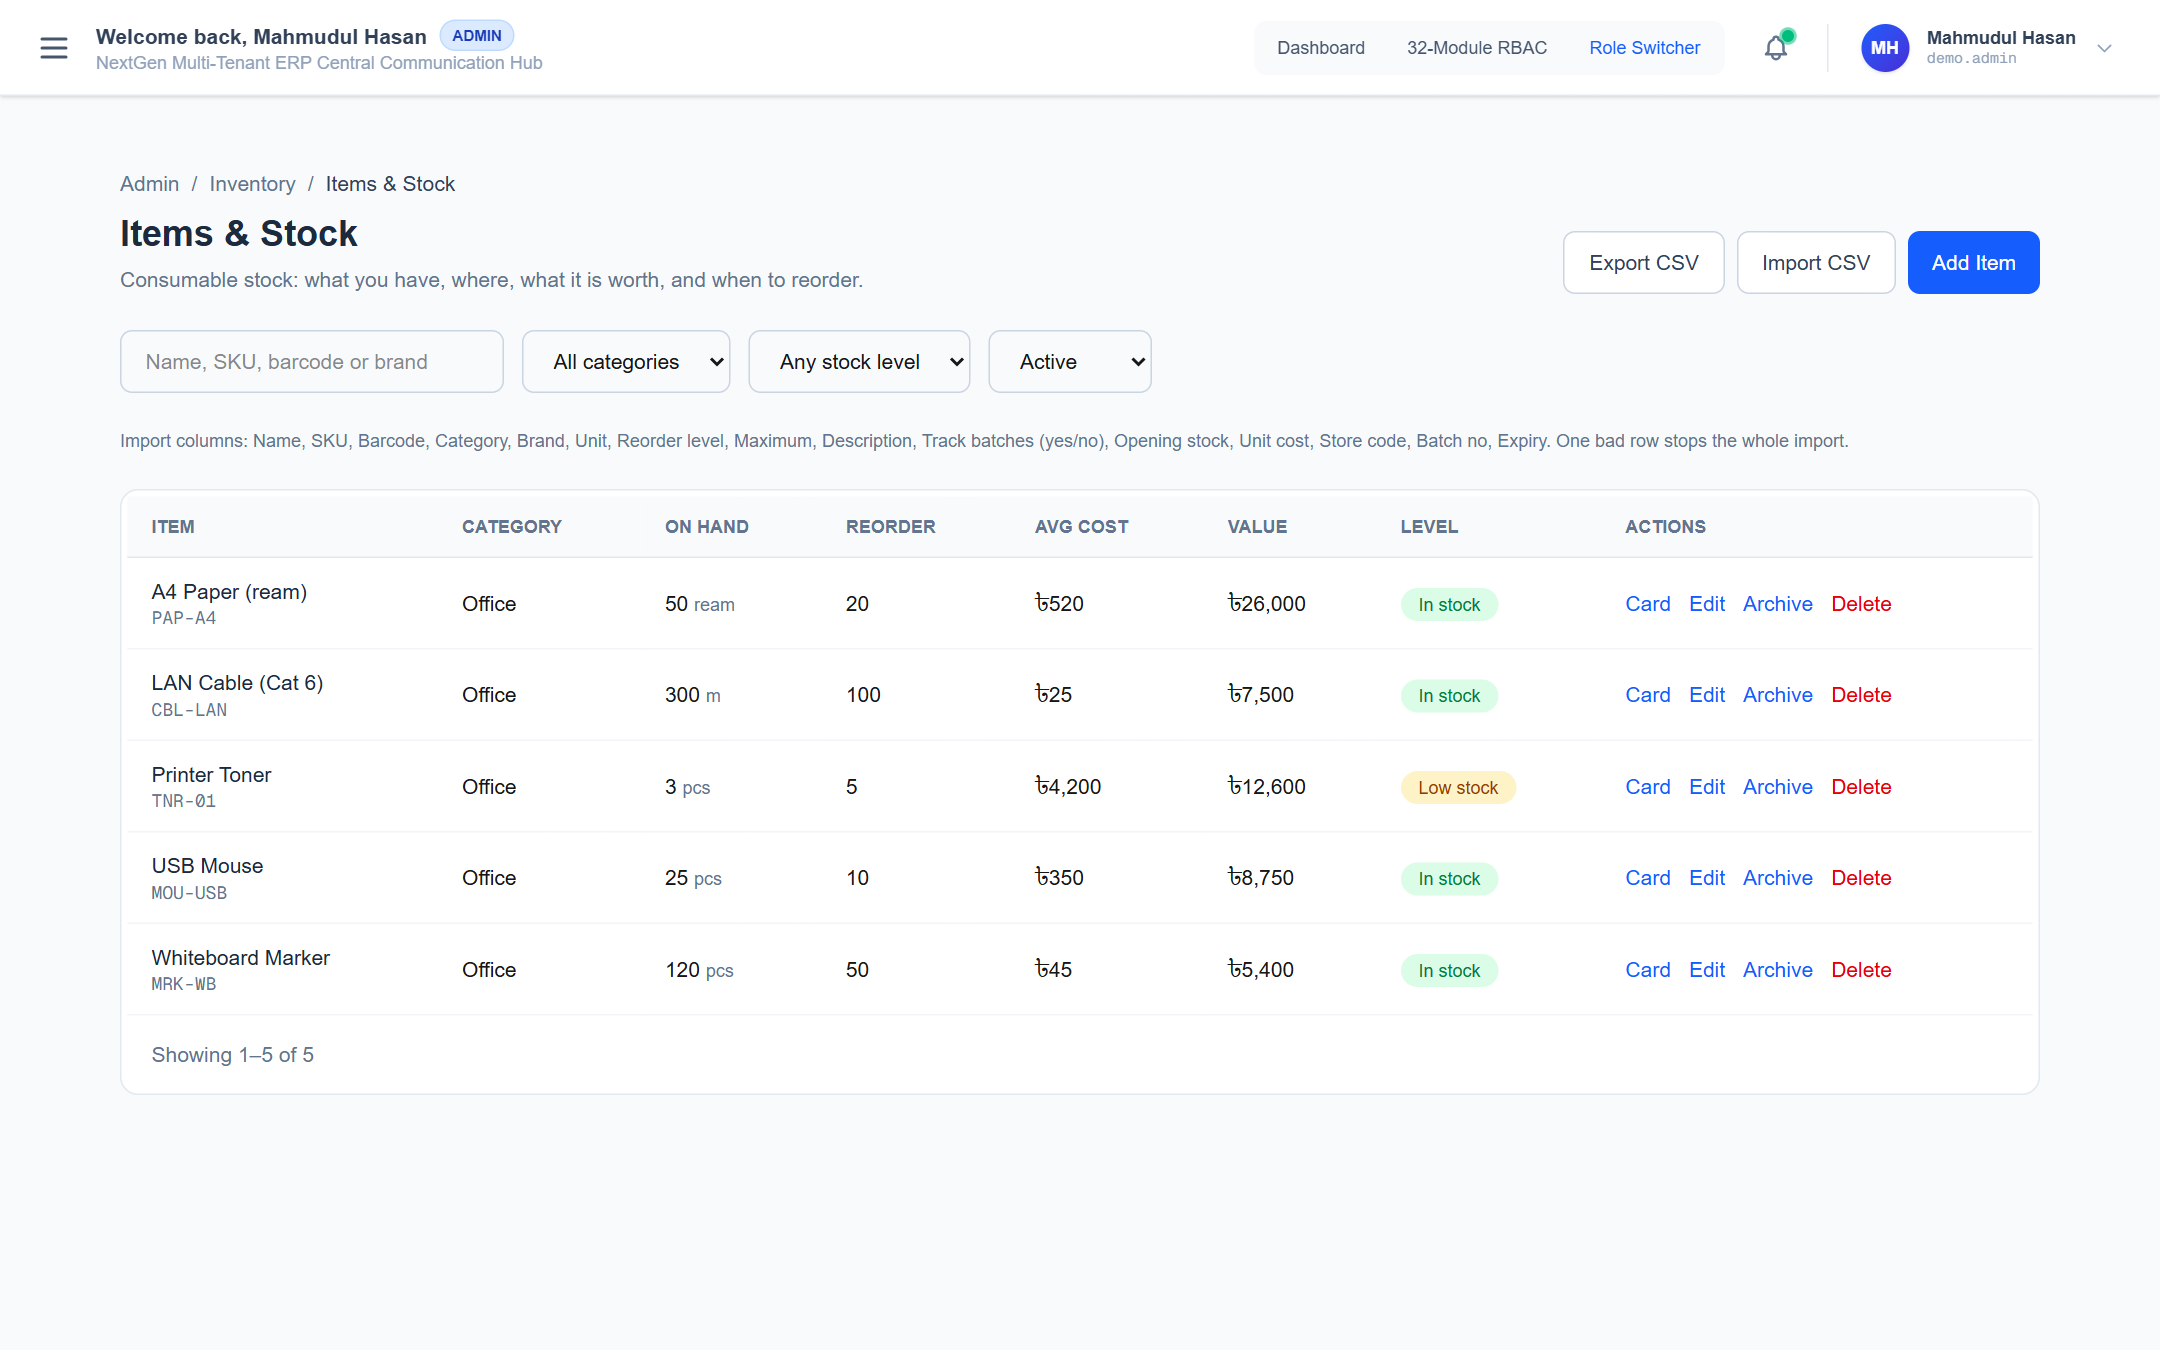
\includegraphics[width=\textwidth]{book_figures/screens/s17_inventory_items.png}
    \caption{Inventory items and stock}
    \label{fig:impl-inventory}
\end{figure}

\section{Notice Management}
The Notices screen in Figure~\ref{fig:impl-notices} lists notices with their category, audience and status. A notice can be saved as a draft or published immediately, and can be sent by email to its audience. The Core API shows each signed-in user only the published notices meant for their audience.

\begin{figure}[H]
    \centering
    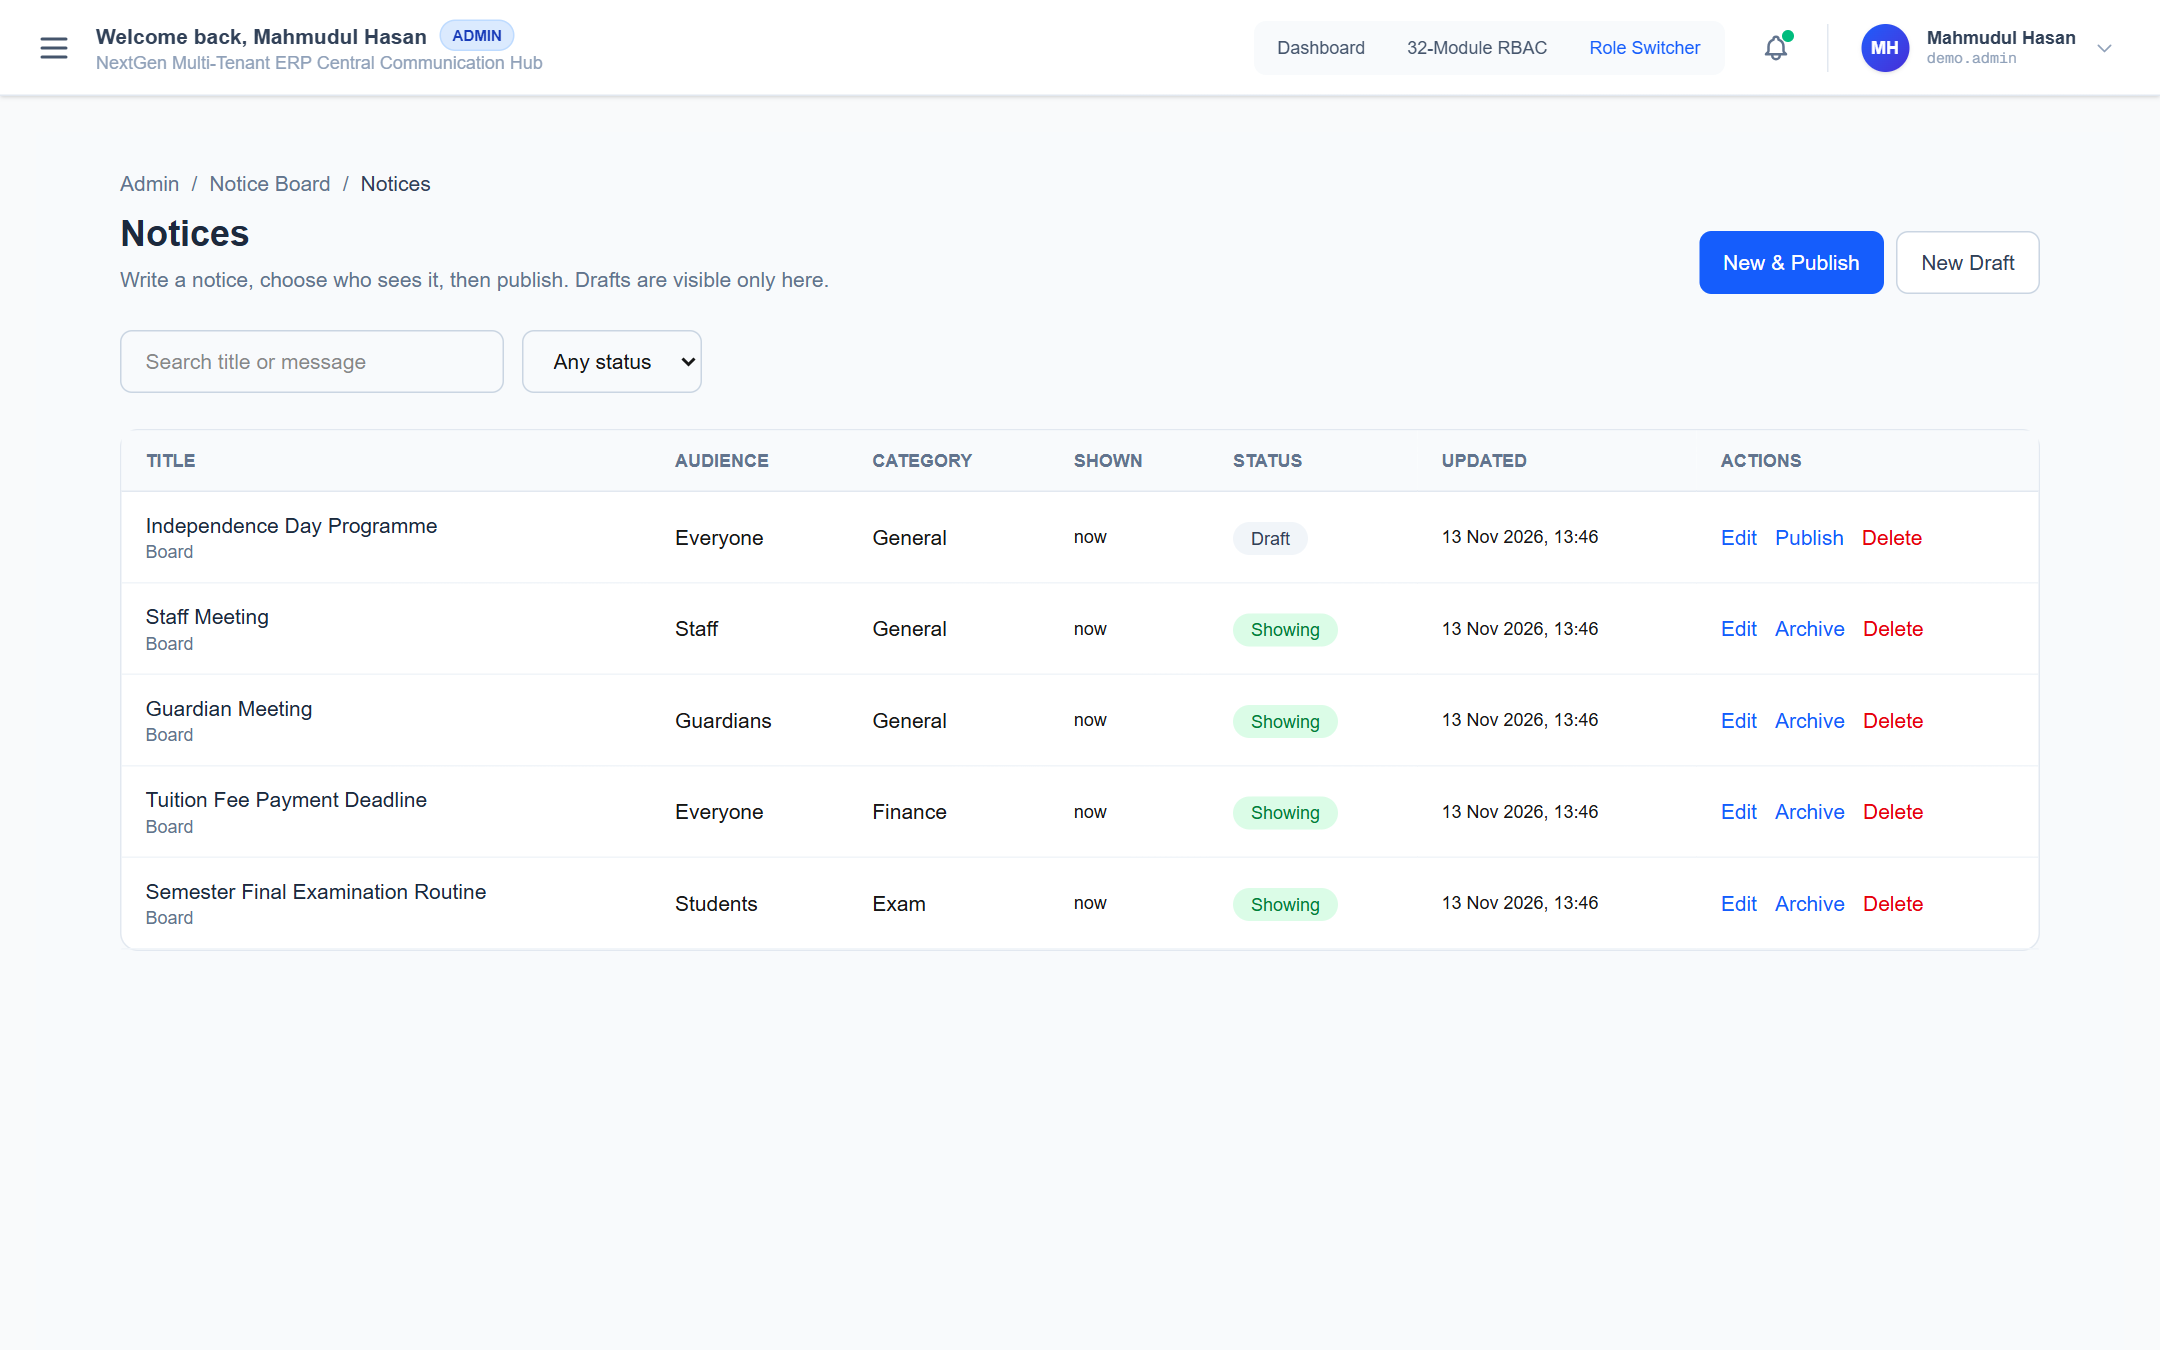
\includegraphics[width=\textwidth]{book_figures/screens/s18_notices.png}
    \caption{Notice management}
    \label{fig:impl-notices}
\end{figure}

\section{Student and Guardian Portal}
Students and guardians use a separate portal page. Figure~\ref{fig:impl-portal-student} shows a student's portal: the hostel seat and rent due, the assistant where the student can type or speak a question, and the notices, results, fees and library sections further down. The conversation in the figure shows three kinds of answers: attendance answered from the student's live records, the library opening hours answered from an approved answer, and a question about results asked in Bangla.

\begin{figure}[H]
    \centering
    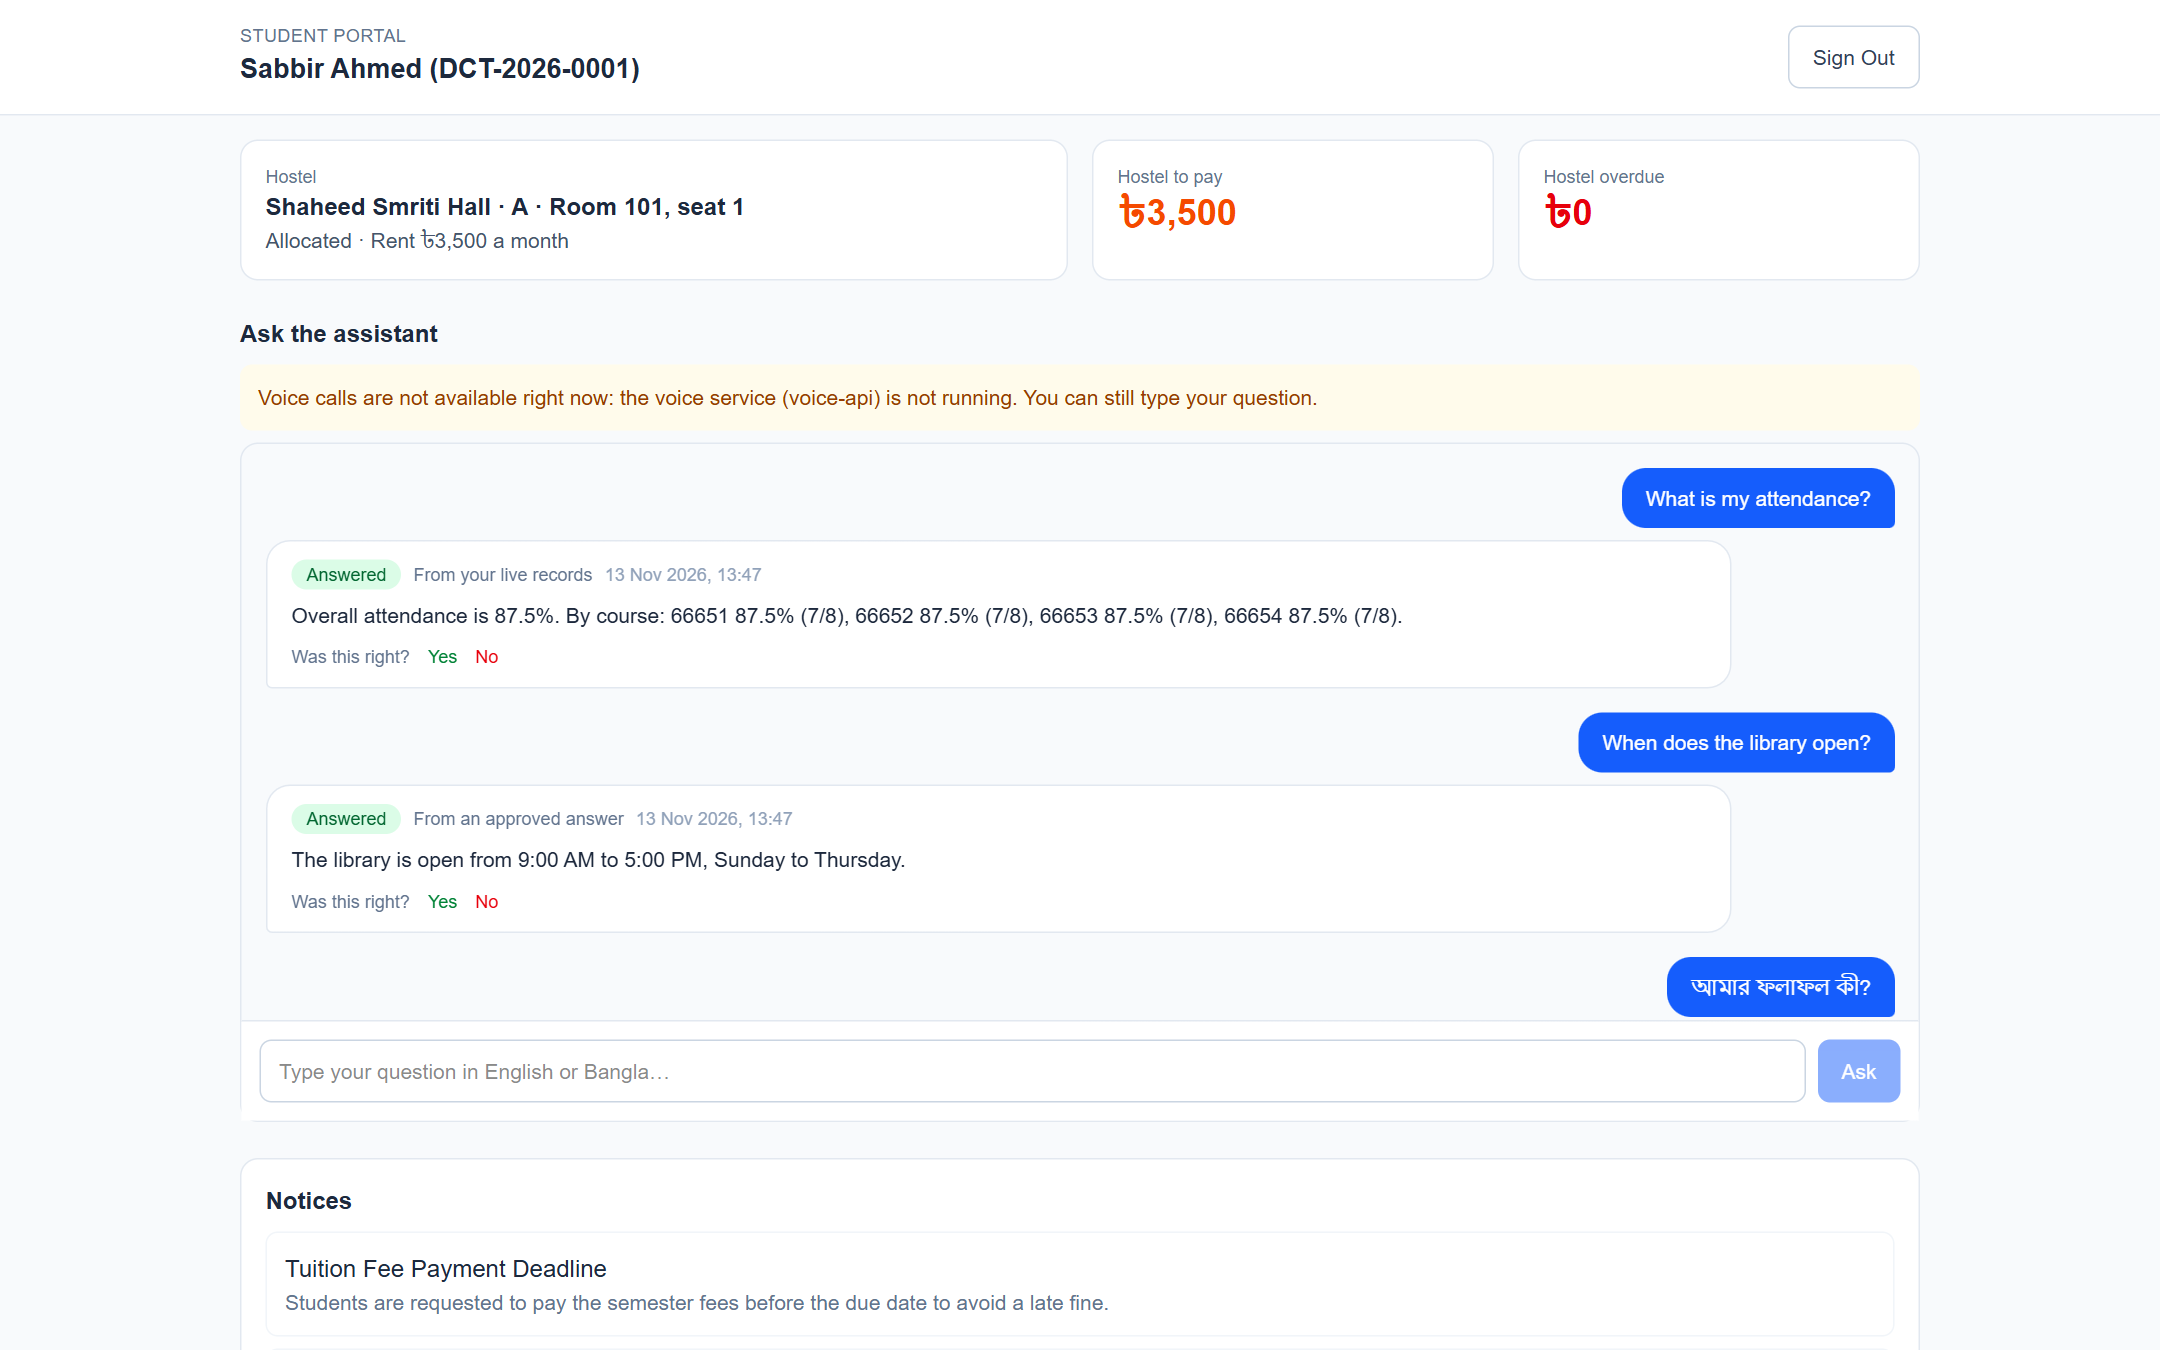
\includegraphics[width=\textwidth]{book_figures/screens/s19_portal_student.png}
    \caption{Student portal with the assistant}
    \label{fig:impl-portal-student}
\end{figure}

Figure~\ref{fig:impl-portal-guardian} shows the portal of a guardian. The guardian chooses one of the linked students and sees that student's records, notices meant for guardians, and the fees and hostel position.

\begin{figure}[H]
    \centering
    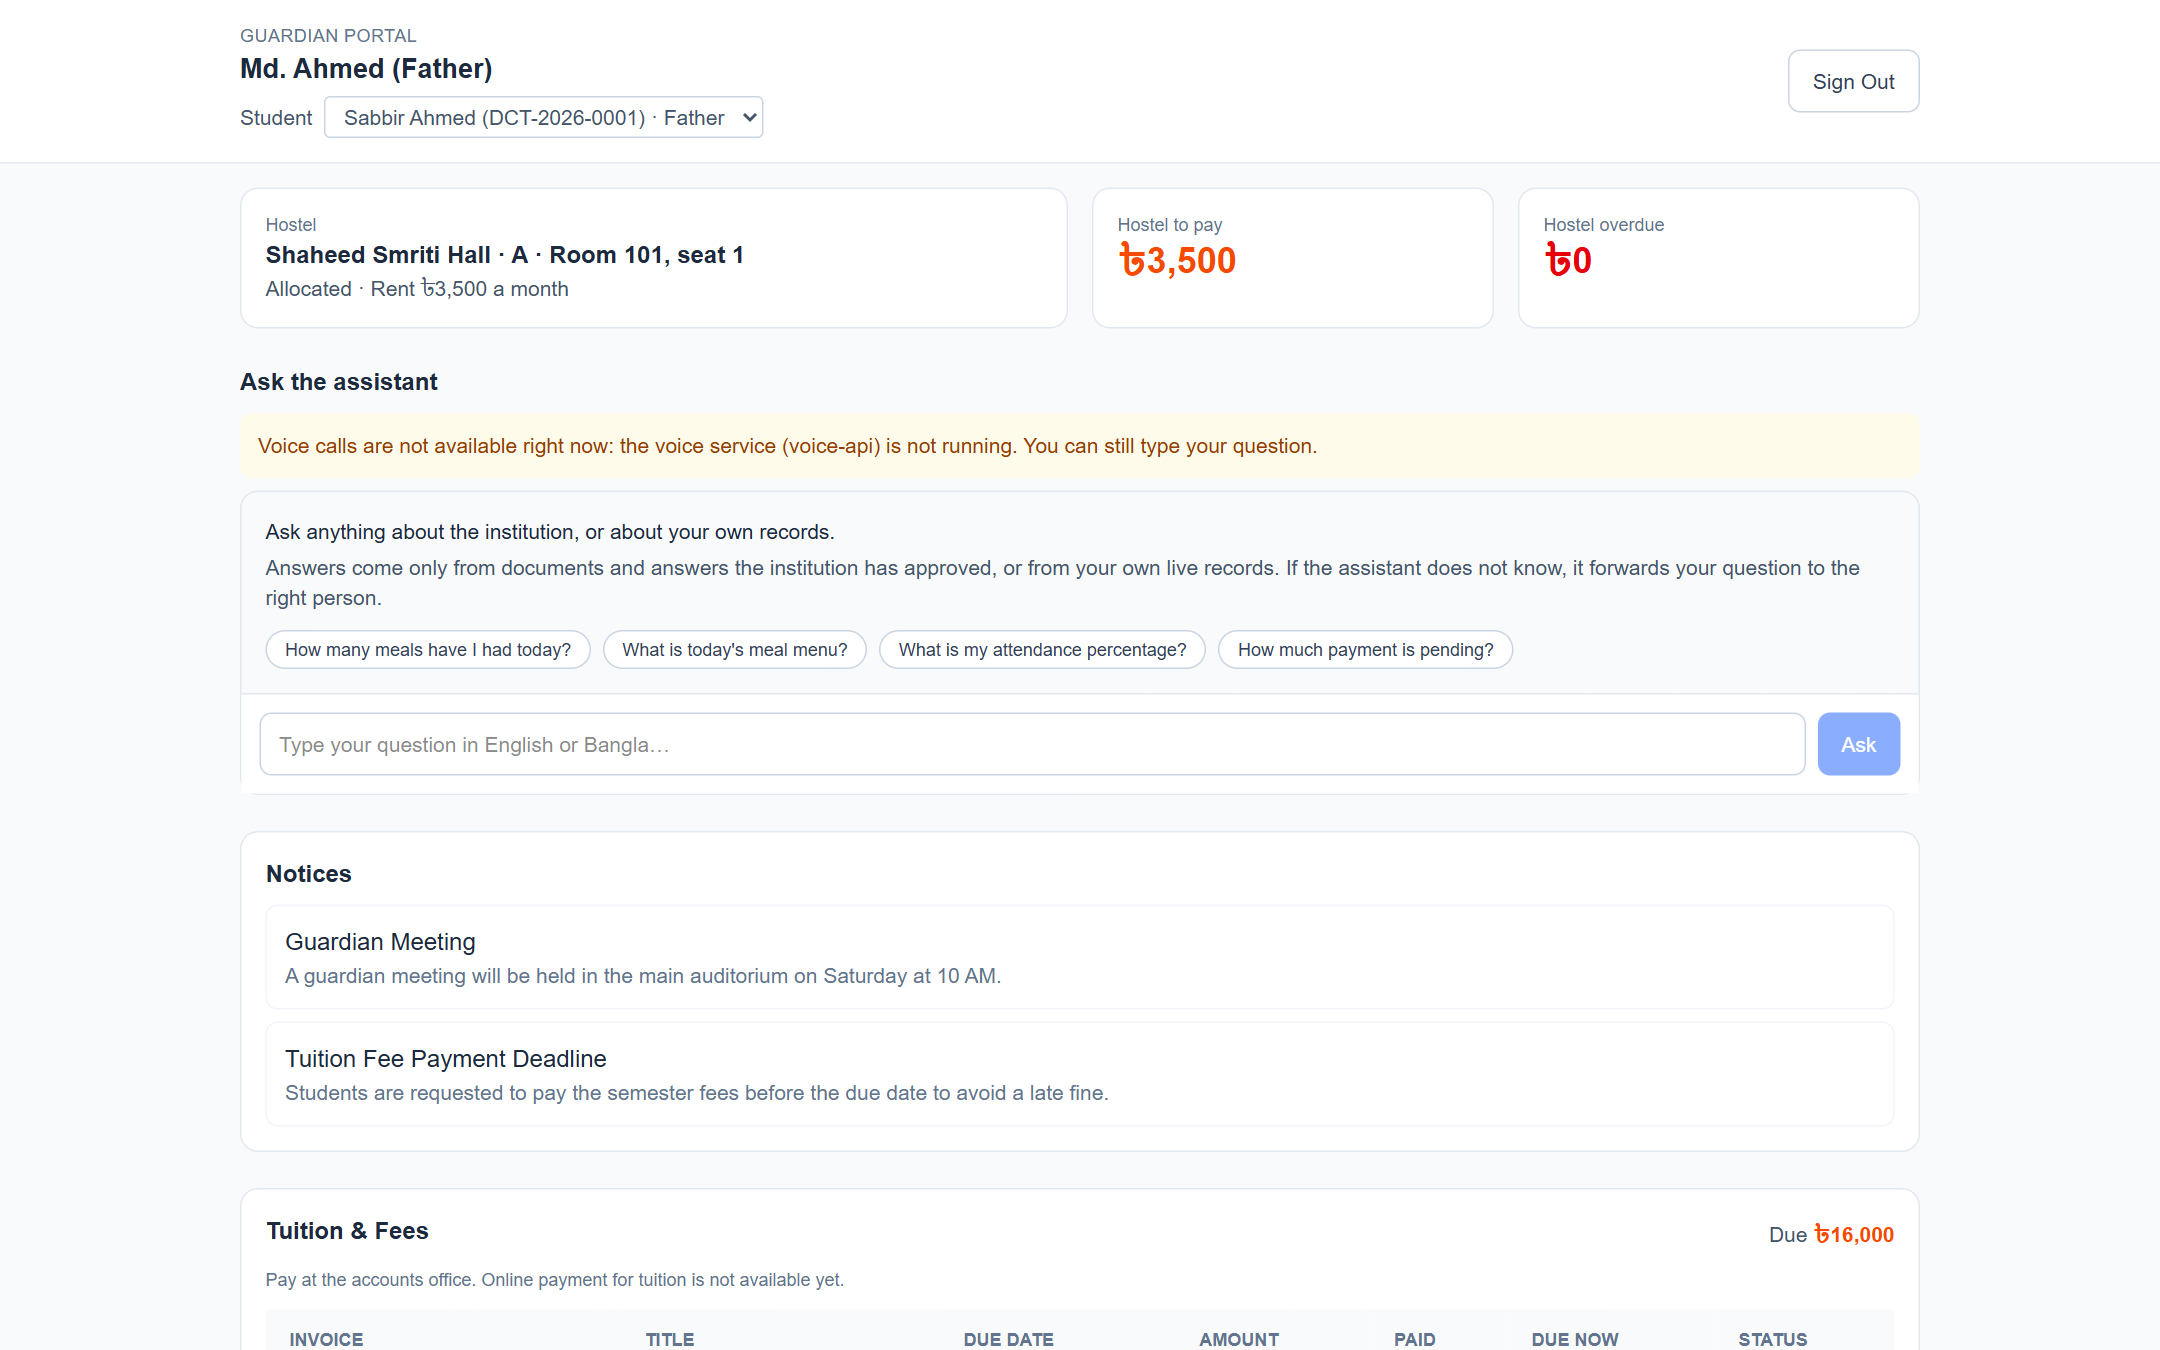
\includegraphics[width=\textwidth]{book_figures/screens/s20_portal_guardian.png}
    \caption{Guardian portal}
    \label{fig:impl-portal-guardian}
\end{figure}

\section{AI Message and Voice Assistant}
Administrators manage the assistant from its own section, shown in Figures~\ref{fig:impl-ask} to~\ref{fig:impl-escalations}. The Ask screen in Figure~\ref{fig:impl-ask} lets staff use the assistant themselves and shows the questions forwarded to them, which they can answer directly from their panel.

\begin{figure}[H]
    \centering
    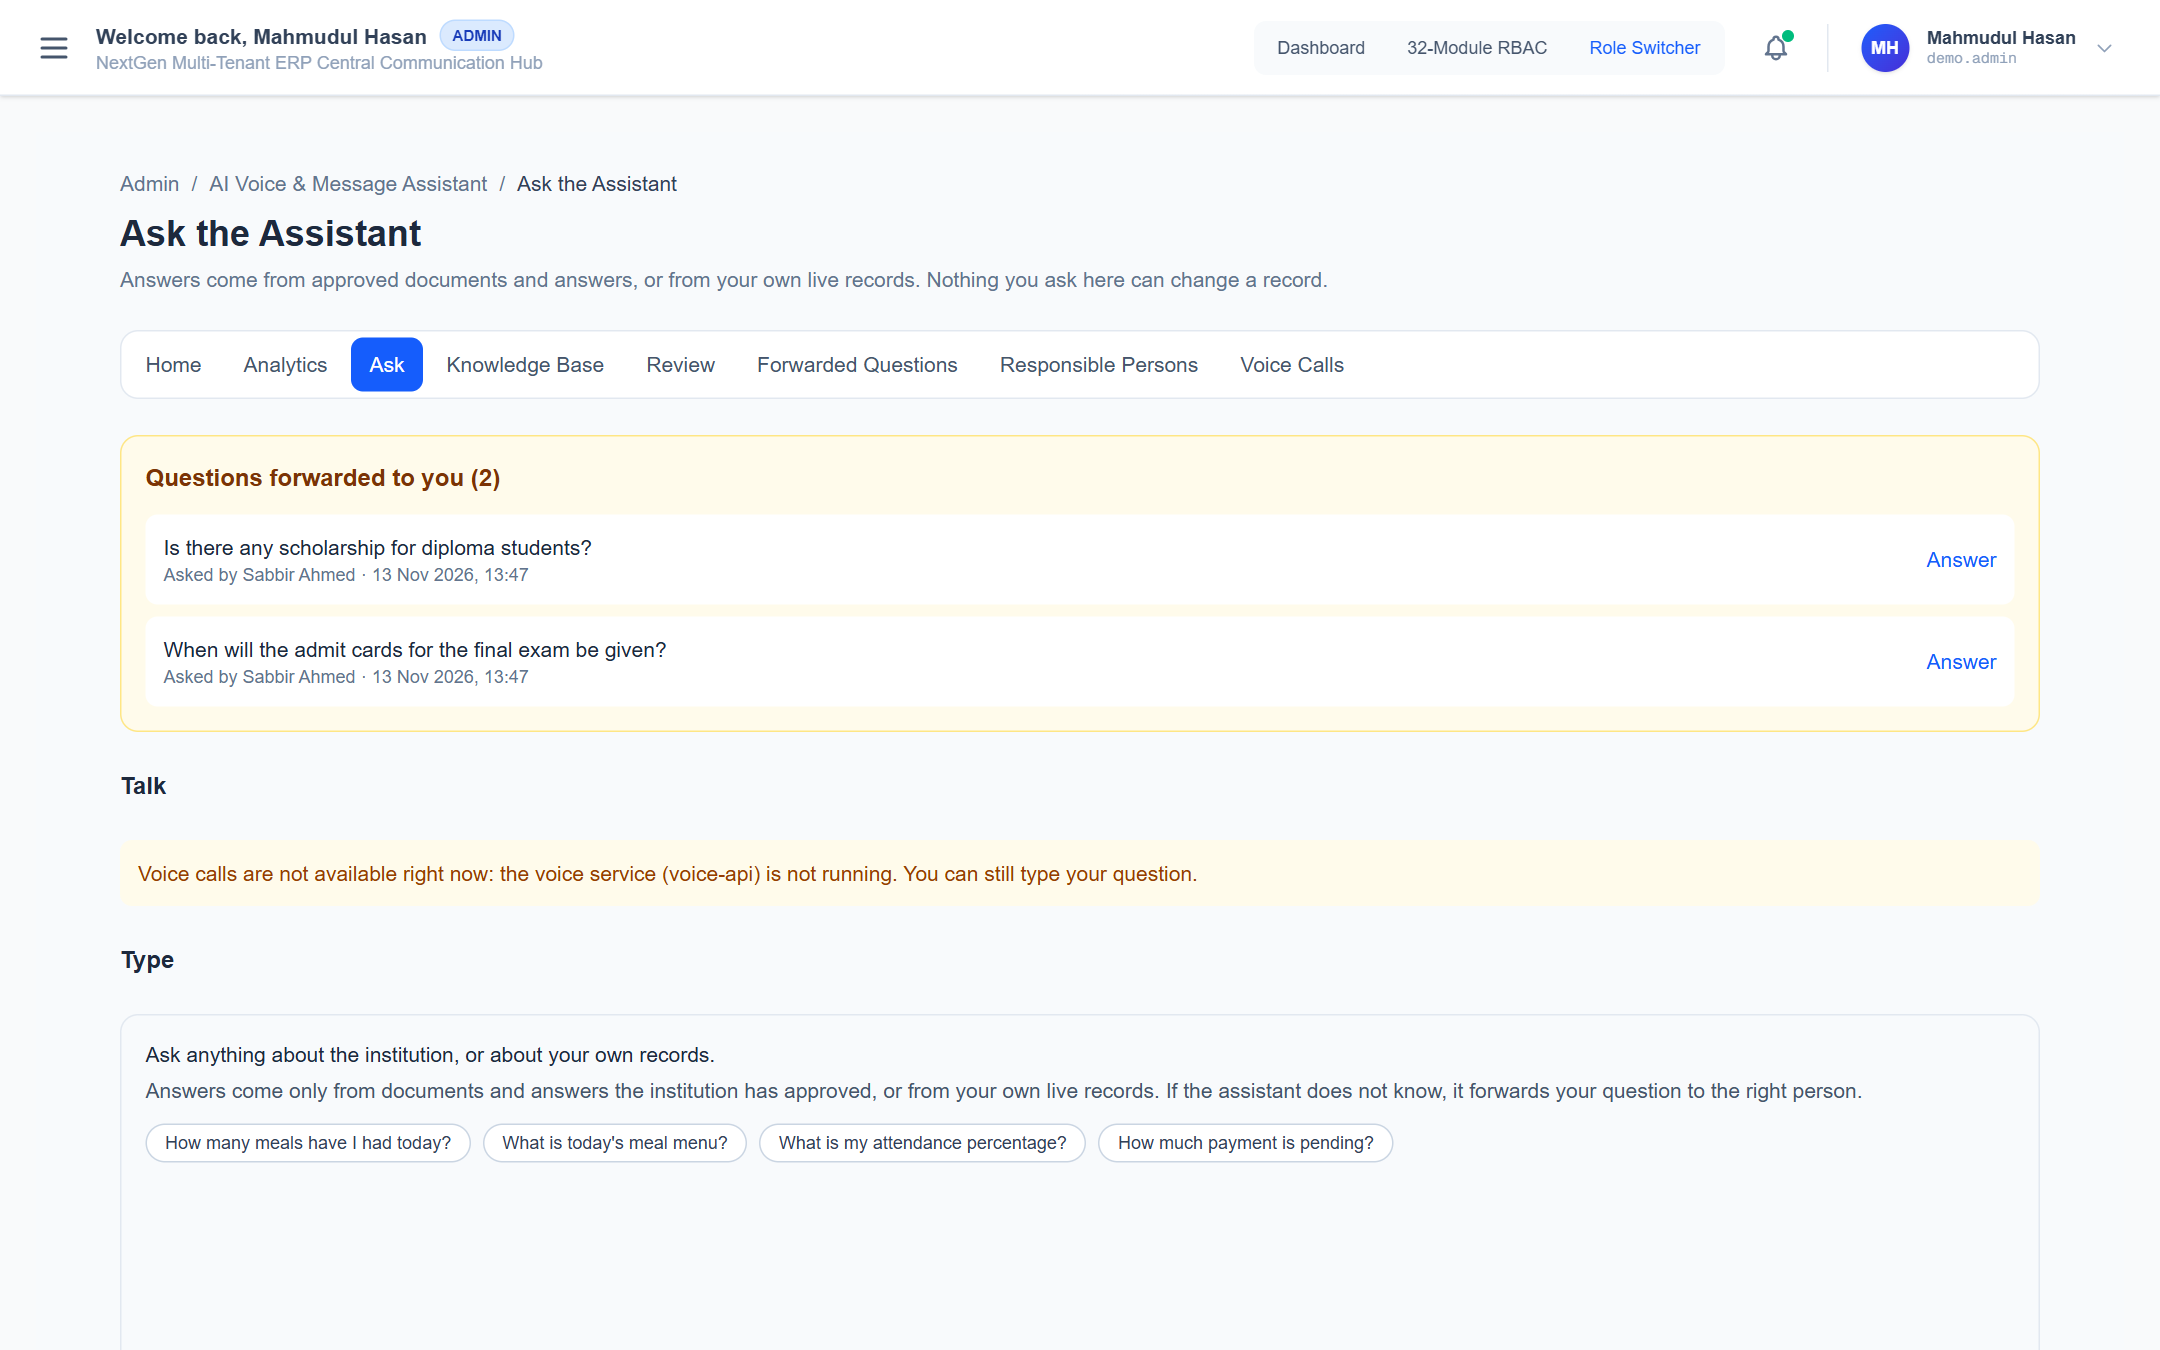
\includegraphics[width=\textwidth]{book_figures/screens/s21_assistant_ask.png}
    \caption{Assistant for staff with forwarded questions}
    \label{fig:impl-ask}
\end{figure}

The Assistant Analytics screen in Figure~\ref{fig:impl-assistant} first shows what is connected: the Voice service, the language model qwen2.5:7b and the bge-m3 embedding model running on the institution's own server through Ollama, and whether SMS, email and call forwarding are set up. It then summarises how questions were handled: how many were asked, answered automatically, answered from live records, forwarded to people or refused, how many answers are approved, and how many documents are ready.

\begin{figure}[H]
    \centering
    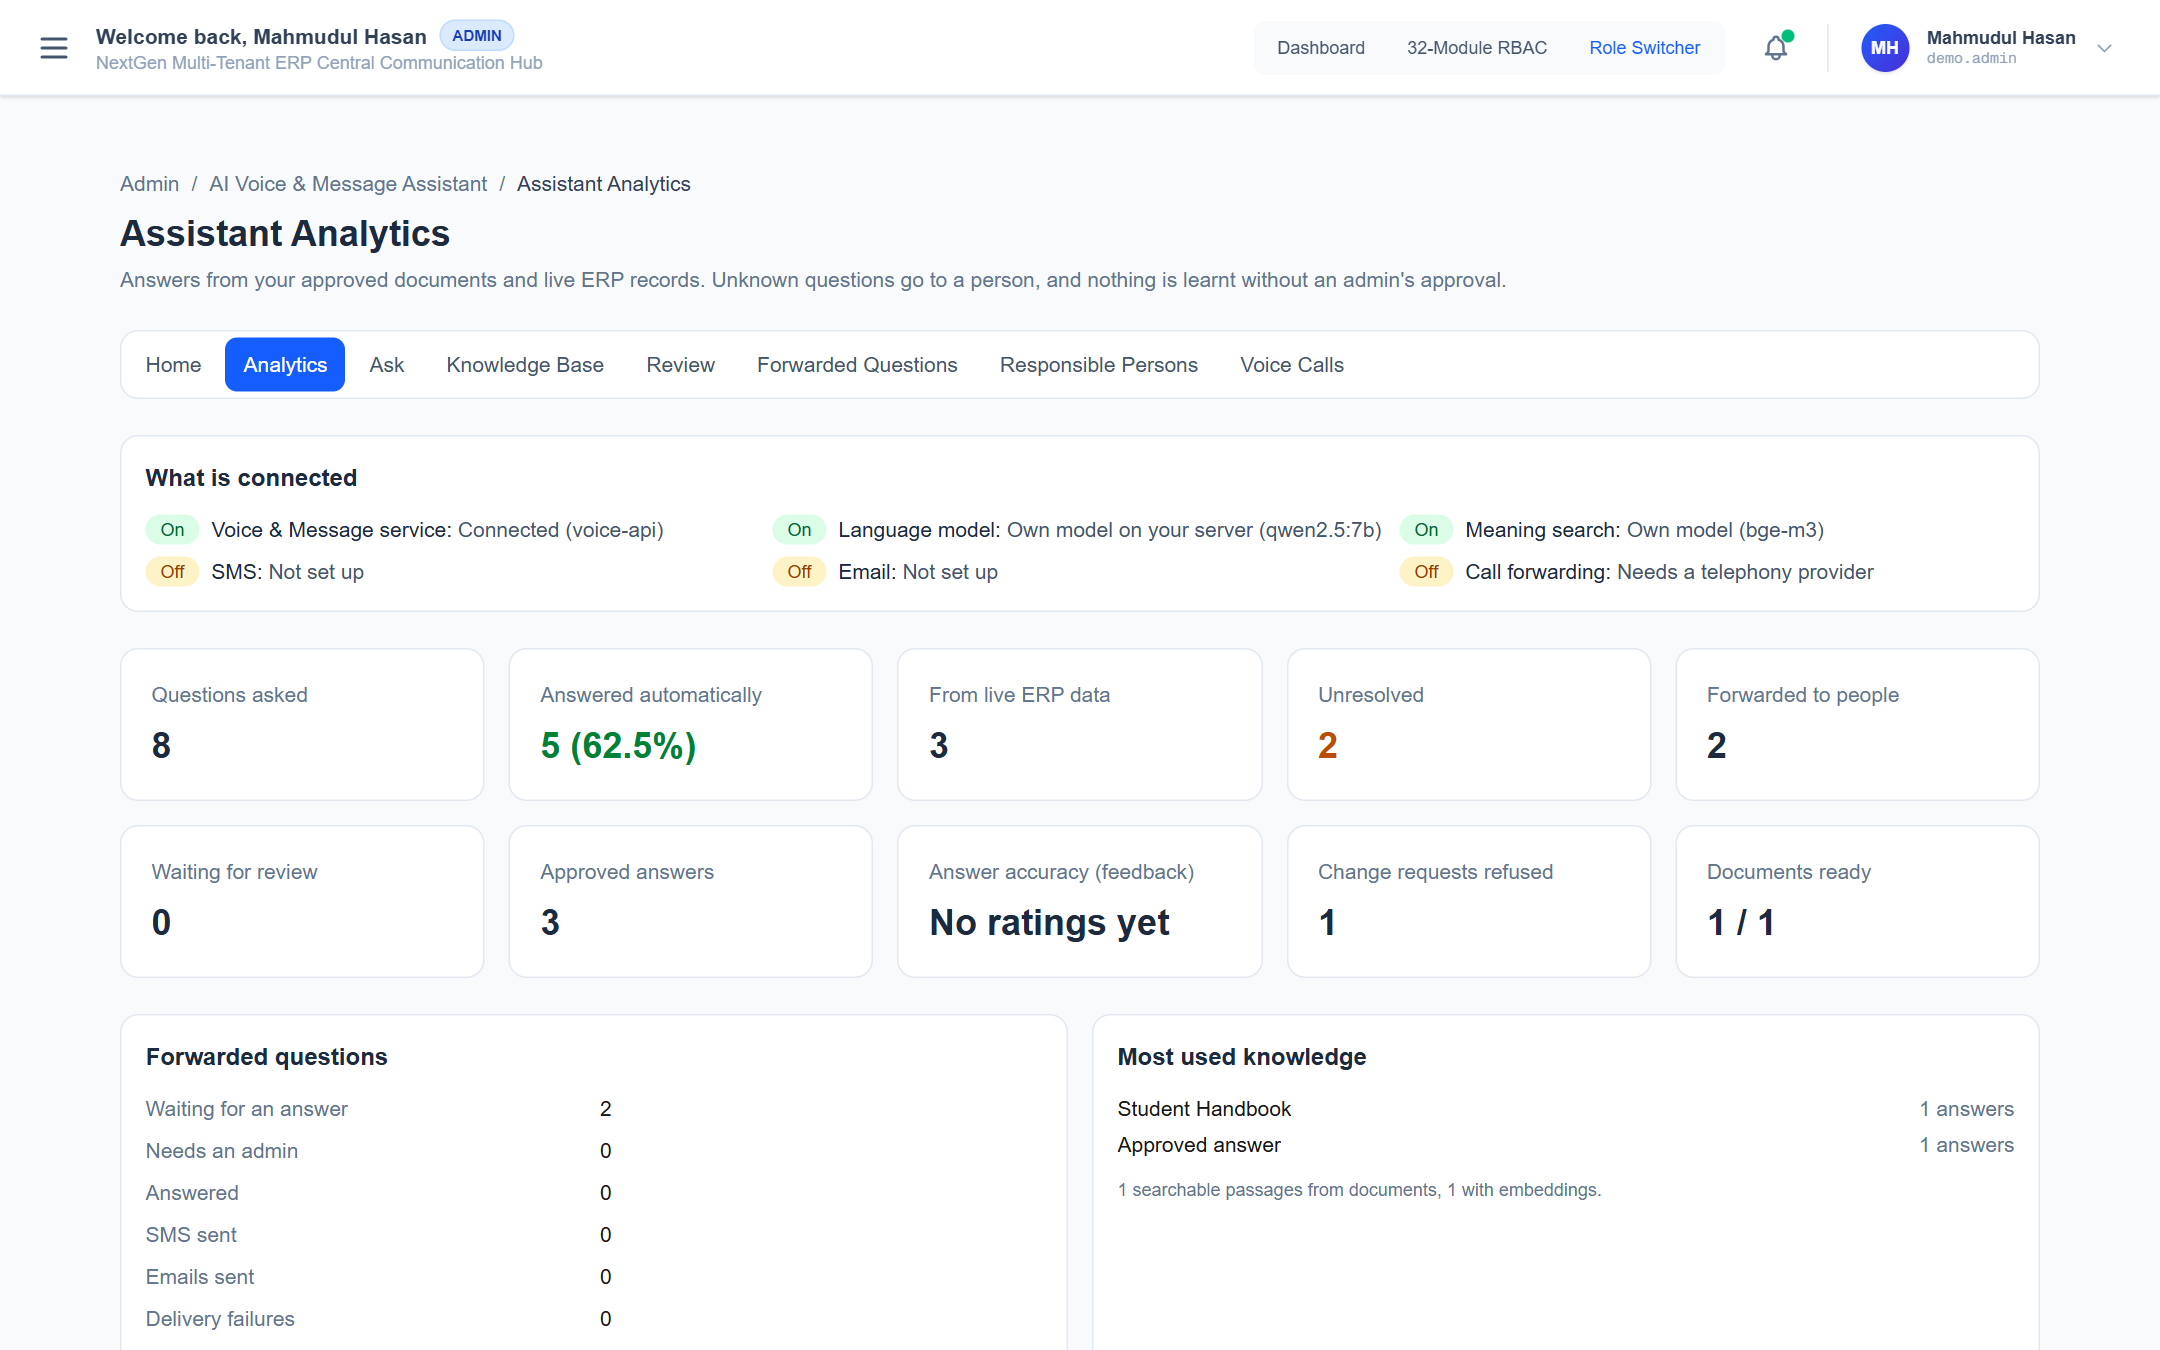
\includegraphics[width=\textwidth]{book_figures/screens/s22_assistant_overview.png}
    \caption{Assistant analytics and connected services}
    \label{fig:impl-assistant}
\end{figure}

The Knowledge Base screen in Figure~\ref{fig:impl-knowledge} lists the uploaded documents with their processing status and the approved answers. In the demonstration, a student handbook was uploaded as a Markdown file; the Voice service read it, the Core API split it into chunks and bge-m3 embeddings were created, after which the language model answered the question ``How many books can a student borrow from the library at a time?'' from the handbook with ``A student may borrow up to three books at a time.''

\begin{figure}[H]
    \centering
    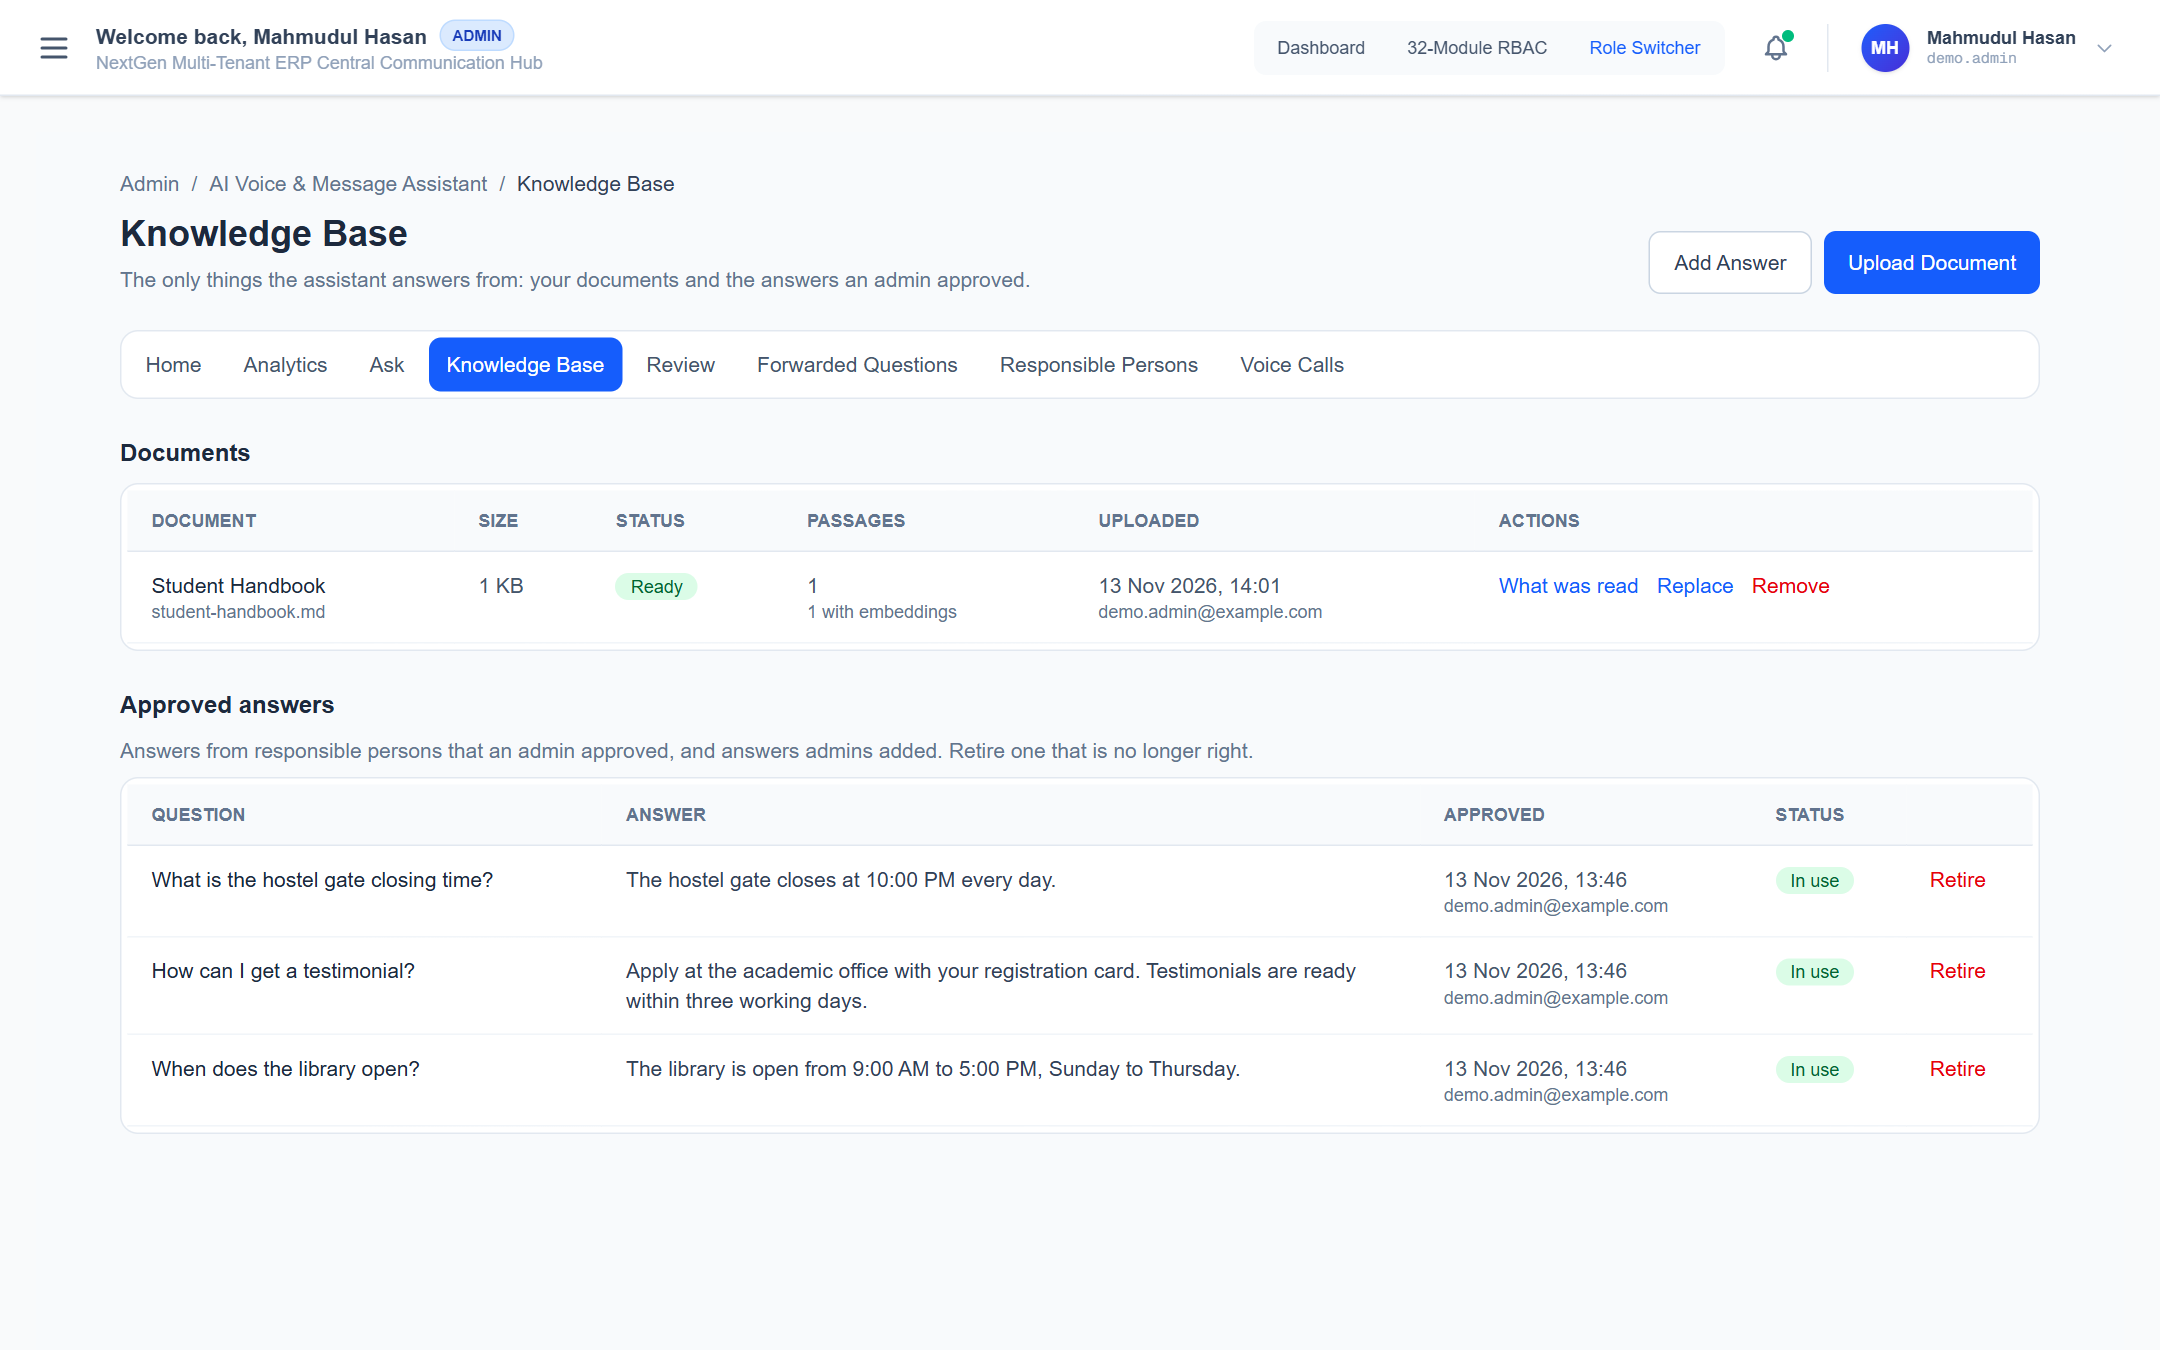
\includegraphics[width=\textwidth]{book_figures/screens/s23_assistant_knowledge.png}
    \caption{Assistant knowledge base}
    \label{fig:impl-knowledge}
\end{figure}

Figure~\ref{fig:impl-voice} shows a voice call in the student portal. The student starts the call, presses the microphone button and asks ``What is my attendance?''. The recording is sent through the Core API to the Voice service, where faster-whisper converts it to text; the Core API answers it from the student's live records, and the Voice service reads the answer aloud with the MMS English voice, which the student can play again. In this demonstration, with the speech models already loaded, the turn took about 20 seconds from the end of the recording to the spoken answer.

\begin{figure}[H]
    \centering
    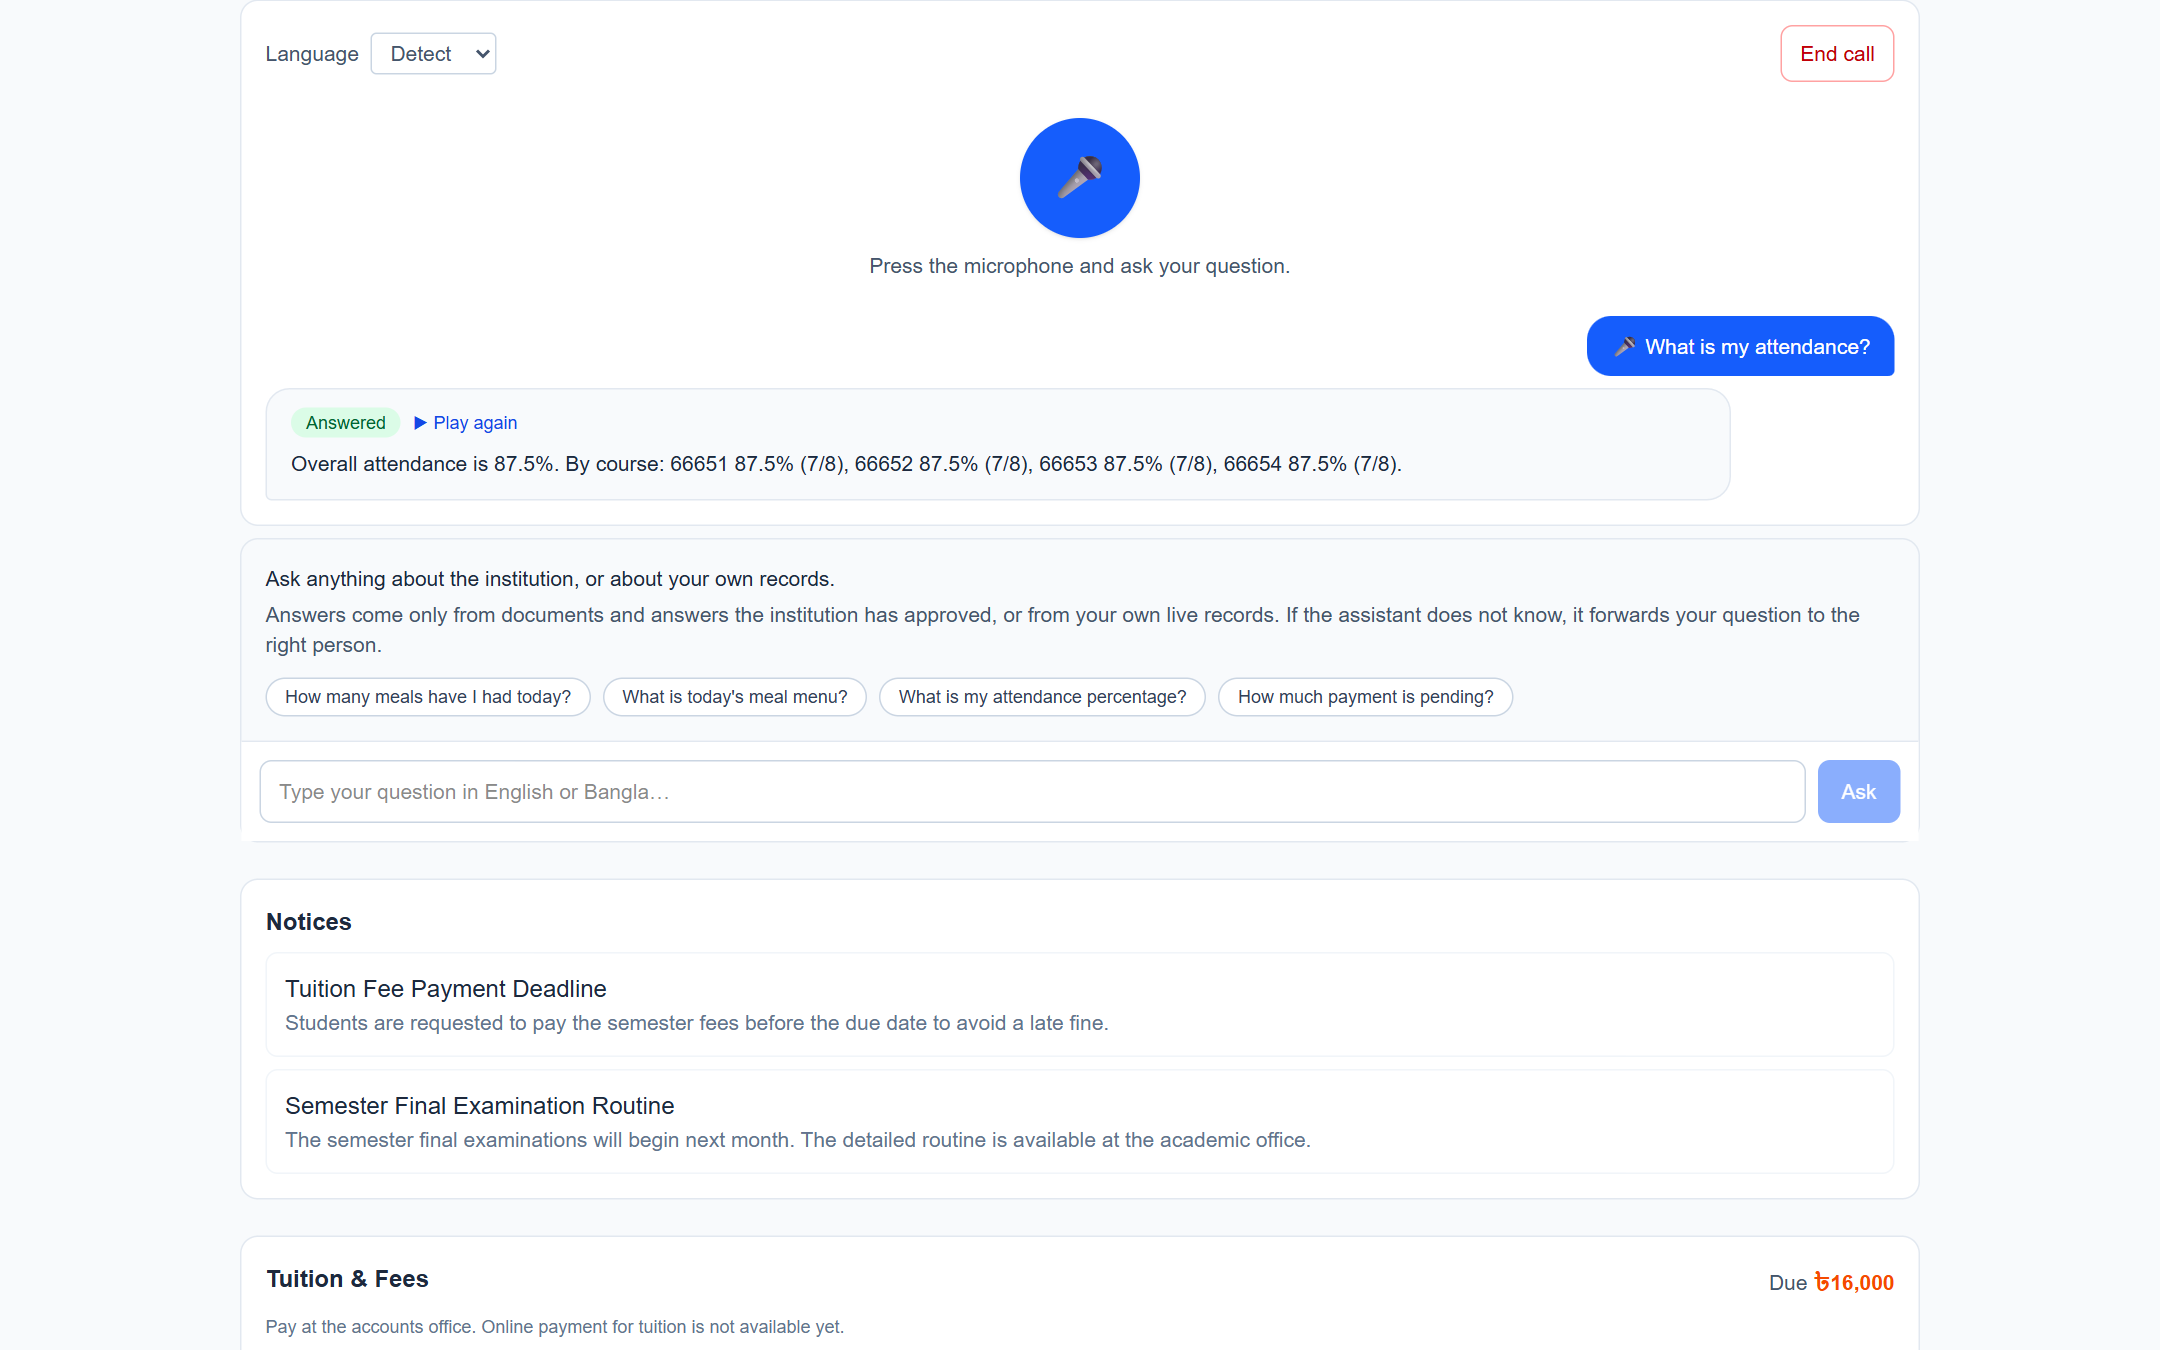
\includegraphics[width=\textwidth]{book_figures/screens/s25_voice_call.png}
    \caption{Voice call with the assistant}
    \label{fig:impl-voice}
\end{figure}

The Forwarded Questions screen in Figure~\ref{fig:impl-escalations} lists the questions that the assistant could not answer, such as when admit cards will be given and whether diploma students can get a scholarship. Each row shows the responsible person, the delivery status on each channel and the actions available to administrators, such as answering on the person's behalf, resending or closing the question.

\begin{figure}[H]
    \centering
    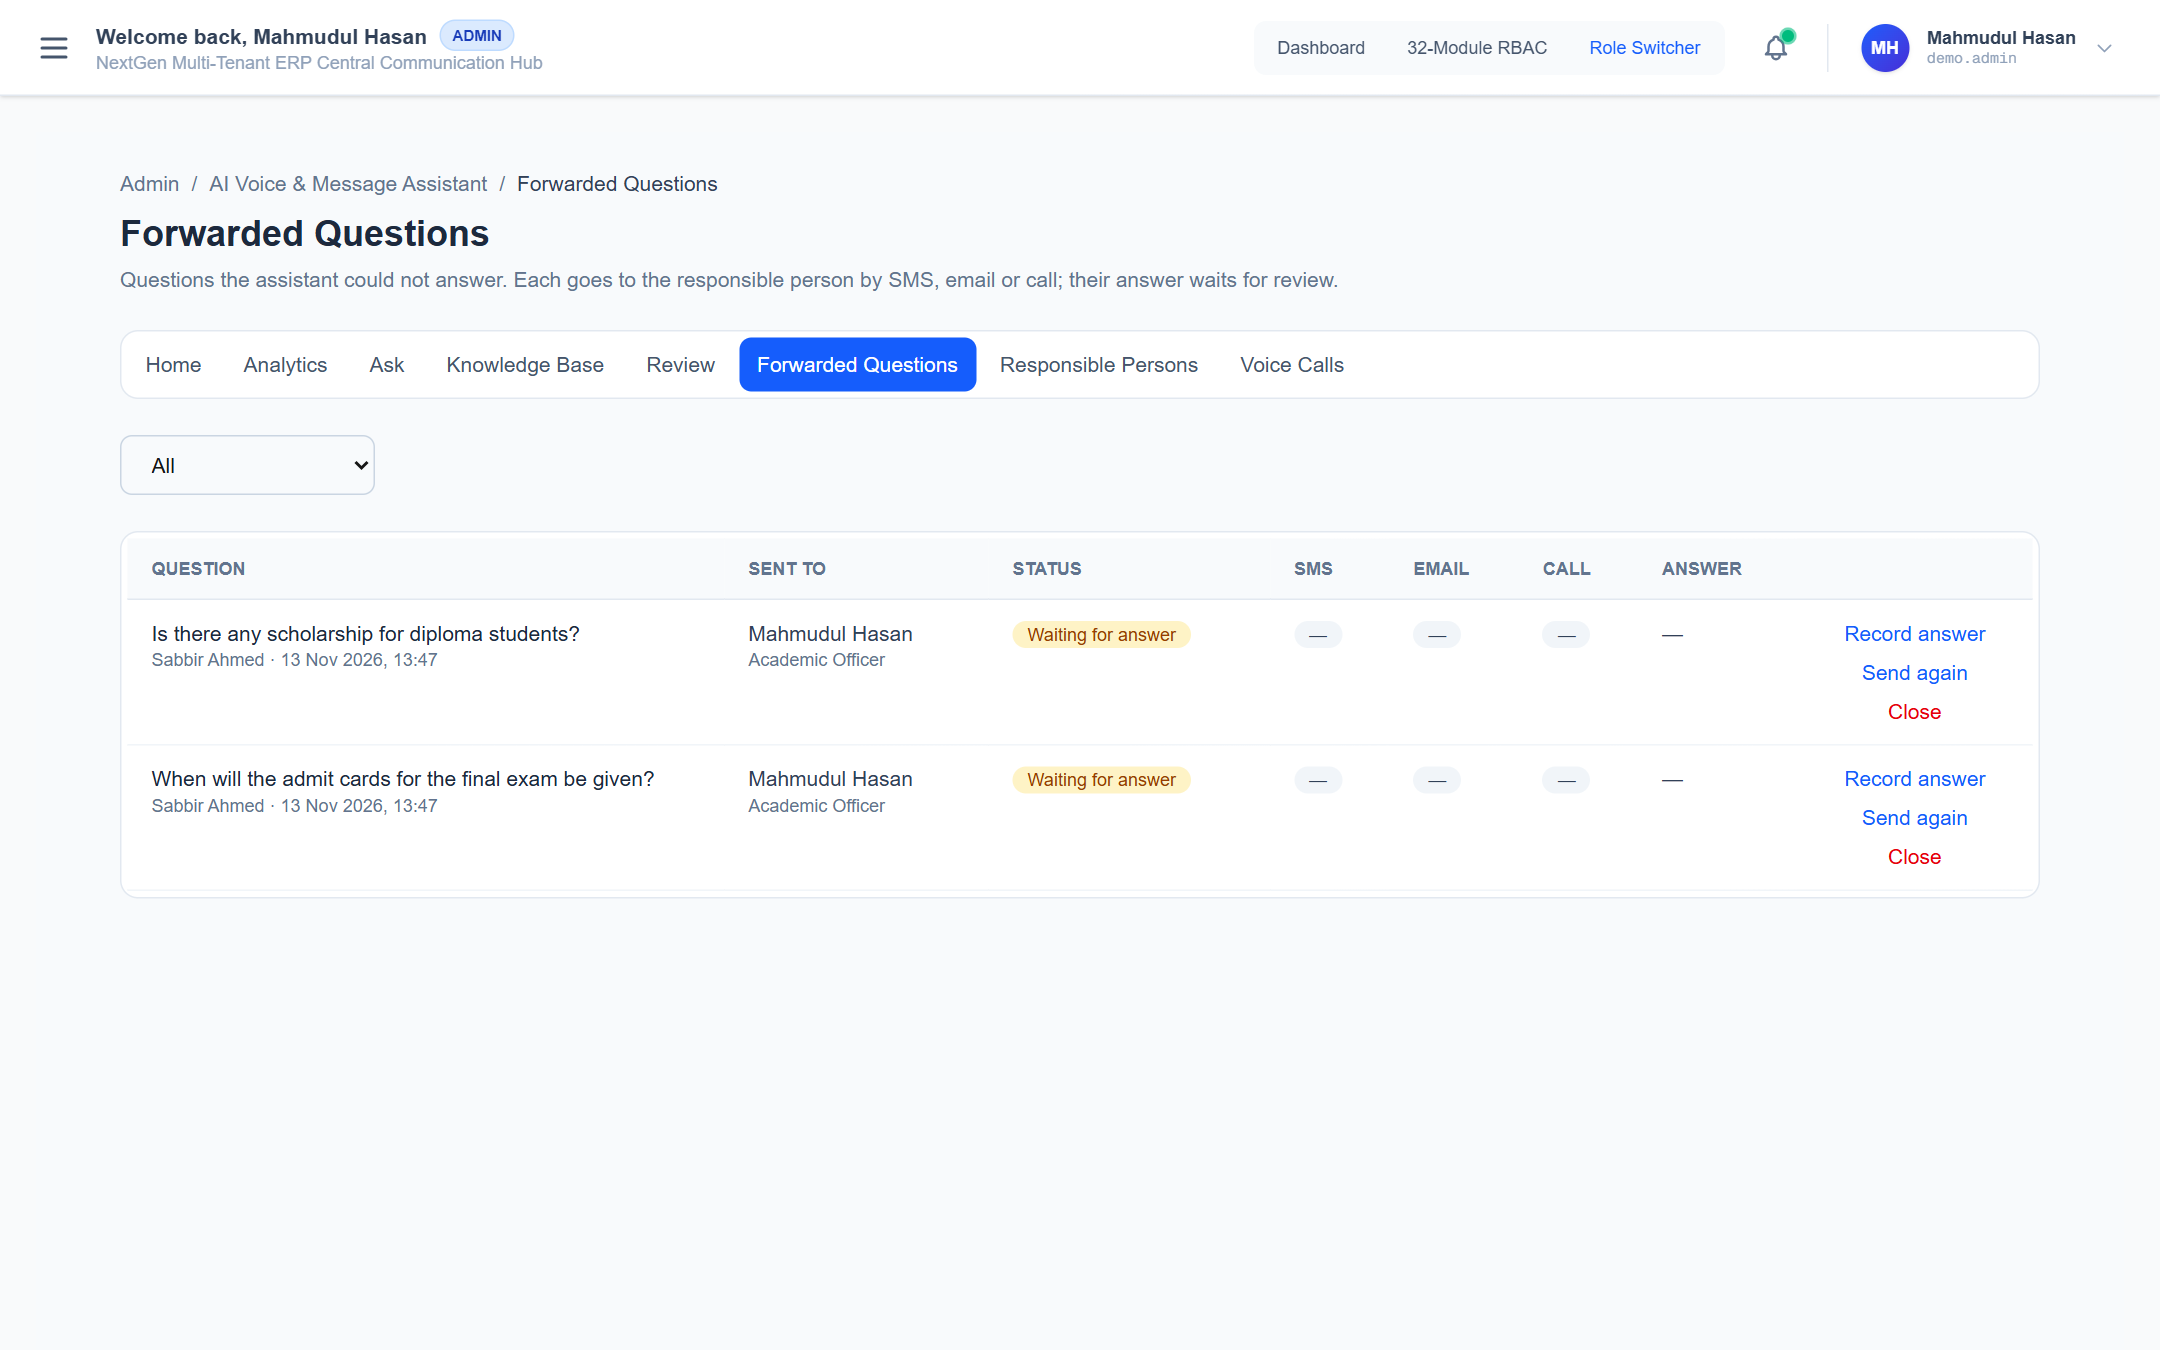
\includegraphics[width=\textwidth]{book_figures/screens/s24_assistant_escalations.png}
    \caption{Forwarded questions}
    \label{fig:impl-escalations}
\end{figure}

\section{Testing and Results}
The automated test suites described in Chapter~V were run on the development machine against the PostgreSQL database in Docker. The results are shown in Table~\ref{tab:test-results}. The Core API suite started the real application, created temporary institutions with their own users, exercised every module through its HTTP interface as different roles, and removed the institutions afterwards. The AI and Voice service suites were run with pytest.

\begin{table}[H]
    \centering
        \caption{Results of the automated tests}
        \label{tab:test-results}
        \begin{tabular}{|p{3.2cm}|c|c|c|c|}
        \hline
        \textbf{Application} & \textbf{Test cases} & \textbf{Passed} & \textbf{Failed} & \textbf{Time} \\
        \hline
        Core API & 128 & 128 & 0 & 178~s \\
        \hline
        AI service & 5 & 5 & 0 & 27~s \\
        \hline
        Voice service & 39 & 39 & 0 & 98~s \\
        \hline
        \textbf{Total} & \textbf{172} & \textbf{172} & \textbf{0} & \\
        \hline
        \end{tabular}
\end{table}

Testing and the demonstration also revealed two defects, which were fixed before the final run. First, when a hostel resident asked the assistant how much fee was due, and the institution had never saved its hostel rent settings, the answer failed with a server error. The assistant reads live records through a read-only database connection, but reading the hostel ledger tried to create the default rent settings. The settings are now read without writing: when no settings exist, the read-only path uses the same values as the database defaults, and a new test checks that these values stay equal to the database's column defaults. Second, a subscription invoice raised after the tenth day of a month, for example when billing was turned on in the middle of a month, was overdue the moment it was created, because its due date was counted from the first day of the period. The due date is now counted from the day the invoice is raised, so every invoice gives the institution ten days to pay, and the billing test checks this.

\section{Deployment}
The system is packaged for deployment with Docker Compose, as shown in Figure~\ref{fig:deployment}. The Core API is built in two stages on a Node.js~20 image, and the AI and Voice services run on Python~3.11 images; the Voice service installs the processor-only build of PyTorch for speech synthesis. The PostgreSQL container loads the database schema on its first start and reports its health, so the Core API starts only after the database is ready. Ollama runs in its own container that is not published outside the internal network, and a one-time container downloads the language and embedding models into a storage volume. The Next.js frontend runs alongside the containers with the development or production Next.js server. The compose file also declares separate databases for the AI and Voice services and a Redis cache, which the current code does not use.

\begin{figure}[H]
    \centering
    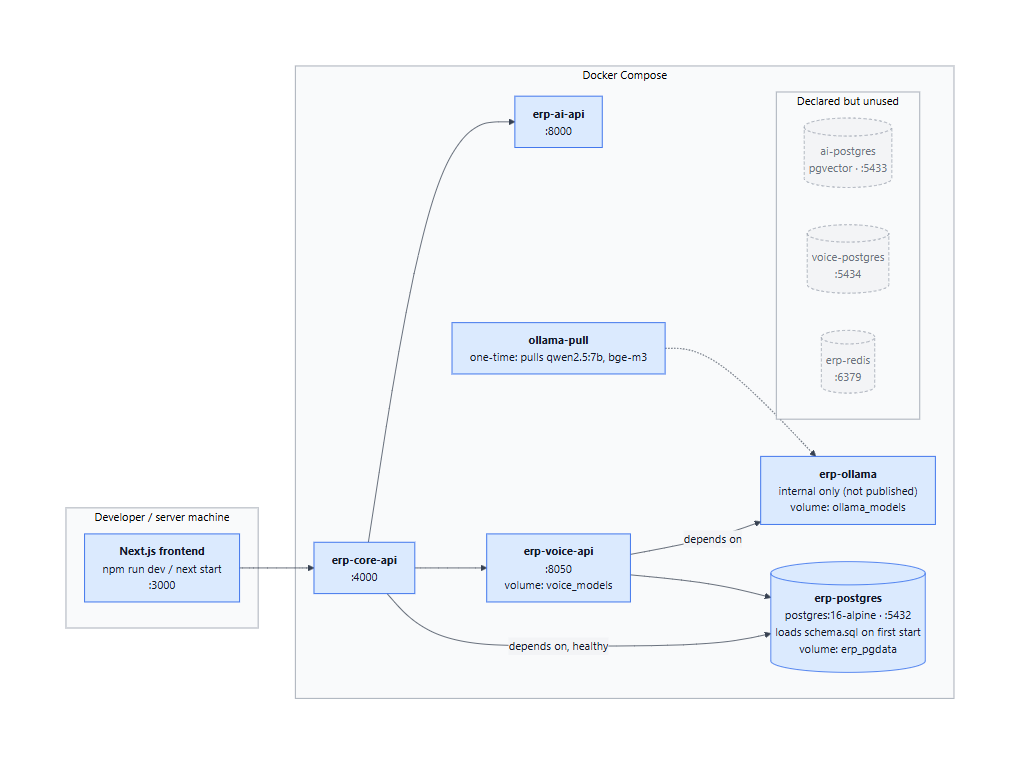
\includegraphics[width=\textwidth]{book_figures/fig02_deployment.png}
    \caption{Container deployment with Docker Compose}
    \label{fig:deployment}
\end{figure}

\section{Summary}
This chapter showed how the designed system was implemented. It presented institution registration and platform management, the sign-in page and dashboard, user, role and permission management, the dynamic form builder, academic structure and student management, attendance, marks entry and results, finance, hostel, library, human resources, inventory and notice management, the student and guardian portal, and the AI message and voice assistant, each with screenshots of the running system filled with demonstration data. It then reported the results of the automated tests, in which all 172 test cases passed, and the two defects found and fixed along the way, and described how the applications are packaged and started with Docker Compose. Together, these implemented features fulfil the objectives set in Chapter~I and lead to the conclusion and future work presented in the next chapter.
